\documentclass[letterpaper,11pt,openany]{book}
\usepackage[centertags]{amsmath}
%\usepackage[pdflatex]{fullbib-bibtex}
\usepackage{graphicx,amsfonts,amssymb,amsthm,newlfont,macros}
\usepackage{tikz}
\usetikzlibrary{shapes.geometric, arrows}
\usepackage{float}
\usepackage{graphics}
\usepackage{caption}
\usepackage{subcaption}
\usepackage{hyperref}
\usepackage{booktabs}
\usepackage{tabularx}\usepackage{biblatex}
\addbibresource{liography.bib}
\usepackage{enumitem}
\setlist[enumerate]{leftmargin=0em}

\newcommand\mat[1]{\boldsymbol{#1}}
\newcommand\vect[1]{\boldsymbol{#1}}
\newcommand\eul{\textup{e}}
\newcommand\imag{\textup{i}}
\makeatletter
% Don't think these are needed so commented them out
%\let\@vwritefile\@writefile
%\def\@ADL@backpage#1{\trelax}
%\newif\ifmtcsecondpart
\@input{classical-control.bux}
\makeatother
\title{MTHE 430 Lab Manual}
\date{\today}
\sloppy 
\begin{document}
\maketitle
\tableofcontents

%\chapter{Introduction to lab equipment}\label{chap:intro}

The purpose of this lab is to introduce the computer programs and the
equipment you will be using in this course.  You will simulate the operation
of an open-loop motor scheme, illustrated in Figure~\ref{fig:openLoop1}\@.
\begin{figure}[htbp]
\centering
\begin{picture}(200,50)
\put(0,22){$u(t)$}
\put(20,25){\vector(1,0){30}}
\put(55,5){\framebox(105,40)
{\large\((\frac{d^2}{dt^2}+\frac{1}{\tau}\frac{d\theta}{dt})=k_Eu\)}}
\put(165,25){\vector(1,0){30}}
\put(196,22){\(\theta(t)\)}
\end{picture}
\caption{Open-loop motor schematic}\label{fig:openLoop1}
\end{figure}%
Hence, the differential equation governing the system is:
\begin{equation}\label{eq:motor}
\frac{d^{2}\theta}{dt^{2}}+\frac{1}{\tau}\frac{d\theta}{dt}=k_Eu.    
\end{equation}
We are interested in the angle, $\theta$\@, and the angular velocity,
$\omega=\frac{d\theta}{dt}$\@, of the motor shaft.  By the end of the lab,
you will have enough data to calculate the motor time constant, $\tau$\@, and
torque constant, $k_{E}$\@.

\section{Key Concepts}
As the first lab is primarily used to have students familiarize themselves with 
laboratory equipment, it does not focus heavily on course related material. 
However, this lab will introduce you to certain applications of Matlab and Simulink 
which will be used continuously throughout all 9 labs in this manual. Simulink is a 
program that allows us to simulate a system, define an input to this system, 
and send the systems output to Matlab. In these labs our system will be a DC motor, 
to which we will be applying various inputs and observing the outputs. Simulink will 
also be used continuously throughout the project portion of the course. 

\noindent You will be using Matlab throughout this course, so start using some best practices. Some useful tips:
\begin{enumerate}
\item \emph{Always} start a script. Whether you are trying to generate plots, simulate dynamics, or do calculations, it is significantly easier to edit, re-use, re-run code in a script as opposed to the workspace.
\item Save your Simulink models to the cloud. This will save you from having the rebuild your model each week.
\item Use a semicolon ``;" to surpress outputs.
\item You can create Section in your script using double percent signs.
\item The \verb|plot| function can handle multiple $x,y$-tuples. Use this to your advantage. The only requirement is that each vector pair has to be the same \emph{length}. You can have multiple $y$ values for one $x$ vector.
\end{enumerate}
\section{Prelab}

It is assumed that the students of this course will have working knowledge of
personal computers. Before you go into the lab, you should read the
following:
\begin{itemize}
\item Appendix~\ref{chap:MATLAB}\@: \textsf{Matlab}\@;
\item Appendix~\ref{chap:hardware}\@: Lab equipment;
\item Appendix~\ref{chap:simulink}\@: \textsf{Simulink}\@;
\item Section 1.2 from the course text.
\end{itemize}

\noindent Before the lab, you must solve the ODE given in Equation~\ref{eq:motor}, for a constant input $u(t)=1$, using an appropriate technique. 
Remember that for an equation of the form $\frac{dy}{dt} + P(t)y(t) = Q(t)$, the integrating factor $\mu(t) = e^{\int P(t)dx}$. Or, you can use Laplace Transformations.\\

\noindent You will be expected to be able to look up material in the appendices during
the course of the various labs, so it is best that you be familiar with what
is in them.  If you are already familiar with any of the topics, you may skip
that section.

\section{Procedure}

The following steps should be followed to set up the simulink models to
properly communicate with the hardware.  You should perform the following
steps \emph{before} adding any blocks to your simulink model to avoid
manually configuring each block in your model.  Concerning any check boxes,
if it is not explicitly stated that you should check a box then it
\emph{must} be left unchecked.
\begin{enumerate}
\item Create the directory 
\begin{center}
\verb|C:\Documents and Settings\<Qlink ID>\My Documents\MATLAB|
\end{center} 
if it does not already exist.
\item Start \textsf{Matlab}.
\item Type \verb|simulink| at the prompt.
\item Click \verb|File|$\to$\verb|New|$\to$\verb|Model| to create a new empty
simulink model.
\item Build a \textsf{Simulink} model (the following steps will guide you
through this) as shown in Figure~\ref{fig:lab1}\@.
\begin{figure}[htbp]
\centering
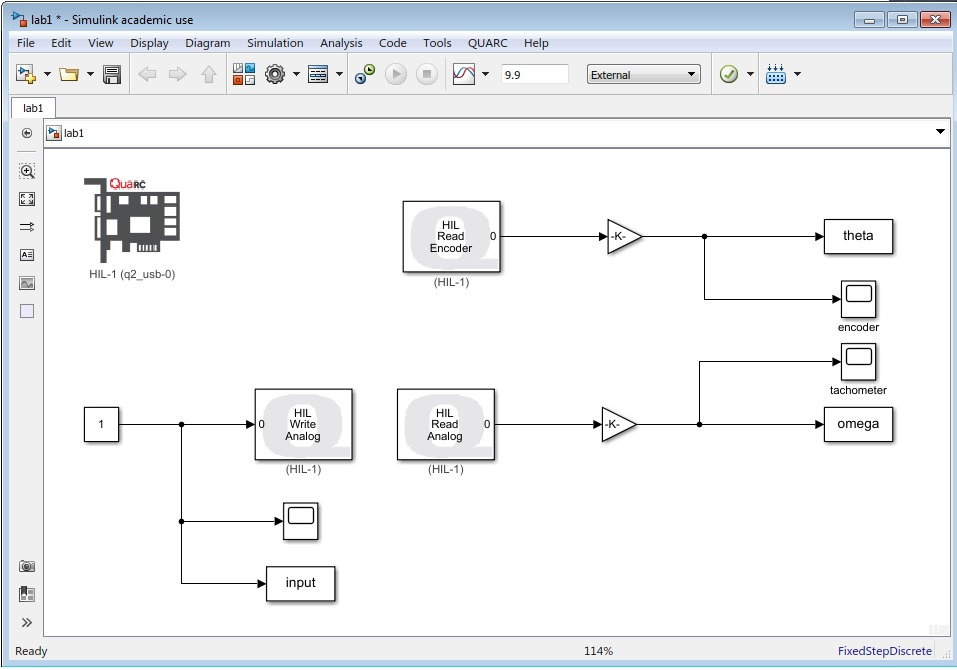
\includegraphics[width=0.9\textwidth]{pix/lab1.PNG} 
\caption{\textsf{Simulink} model for Lab~\ref{chap:intro}}\label{fig:lab1}
\end{figure}%
The model applies a constant voltage to the servomotor.  The encoder is
employed to acquire the angular position ($\theta$) and the tachometer is
used to acquire the angular velocity ($\omega$) as functions of time.
\item Make a new folder on the hard drive under the name or number of your
group and save your model under the name \verb|lab1_name_of_your_group.mdl|.
Save all files created (e.g., model file, plots) in each lab session in that
folder.  It might be a good idea to create a folder for each lab session as
well.

\item Drag the \verb|HIL Initialize| block from the library window into the
model.  You can find this block under:
\begin{center}
\verb|QuaRC Targets|$\to$\verb|Data Acquisition|$\to$\verb|Generic|$\to$\verb|Configuration|
\end{center}
\item Double click on the new \verb|HIL Initialize| block in your model to
configure the parameters.
\begin{enumerate}
\item Main Tab
\begin{itemize}
\item Board Type = \verb|q2_usb|
\end{itemize}
\item Encoder Inputs Tab
\begin{itemize}
\item Encoder Input Channel = \verb|[0]|
\item Encoder Quadrature = \verb|[4]|
\item Encoder Frequency in Hertz = \verb|[ ]|
\item Initial Encoder Counts = \verb|0|
\item Check box \verb|Set encoder input parameters at model start|
\item Check box \verb|Set initial encoder counts at model start|
\end{itemize}
\item Analog Outputs Tab
\begin{itemize}
\item Analog Output Channels = \verb|[0]|
\item Initial Analog Outputs = \verb|0|
\item Final Analog Outputs = \verb|0|
\item Analog Outputs on Watchdog Expiry = \verb|0|
\item Check box \verb|Set initial analog outputs when switching to this model|
\item Check box \verb|Set final analog outputs at model termination|
\item Check box \verb|Set final analog outputs when switching from this model|
\end{itemize}
\end{enumerate}

\item Click \verb|Apply| and then \verb|OK| to close the properties dialog box.

\item Once the \verb|HIL Initialize| block is set up properly, you can add
blocks to your simulink model to read and write analog signals to the
interface board.  The main blocks of interest are \verb|HIL Read Encoder|,
\verb|HIL Read Analog| and \verb|HIL Write Analog|, which replace the old
blocks \verb|Encoder Input|, \verb|Analog Input| and \verb|Analog Output|,
respectively.  Consult the instructions to see which blocks to use in each
lab. There are no \verb|calibration|, \verb|encoder|, or \verb|tachometer|
blocks.  These blocks are simply ``gain'' or ``scope'' blocks which have been
renamed.  It is always best to refer to the block pictures instead of the
block names.  These blocks can be found at
\begin{center}
\verb|QuaRC Targets|$\to$\verb|Data Acquisition|$\to$\verb|Generic|$\to$\verb|Immediate I/0|
\end{center}
\begin{center}
\verb|Simulink|$\to$\verb|Commonly used blocks|
\end{center}
When using the HIL \verb|Read Analog| block, make sure that the correct
channel is set (channel \verb|0|).
\begin{figure}[htbp]
\centering
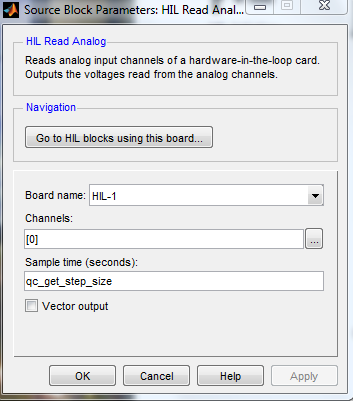
\includegraphics[width=0.5\textwidth]{pix/hil-read-analog-block.PNG}
\caption{HIL \texttt{Read Analog} block settings}\label{fig:hilrab}
\end{figure}
\begin{figure}[htbp]
\centering
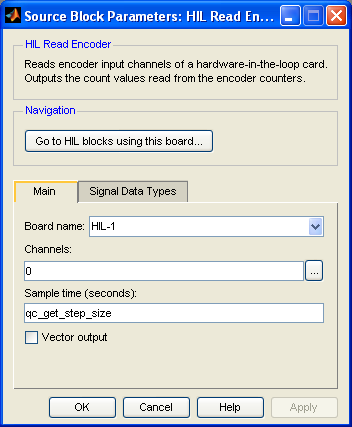
\includegraphics[width=0.5\textwidth]{pix/hil-read-encoder-block.PNG}
\caption{HIL \texttt{Read Encoder} block settings}\label{fig:hilreb}
\end{figure}
\begin{figure}
\centering
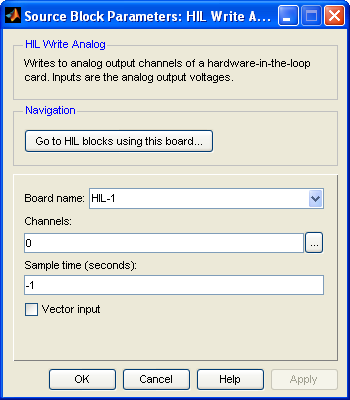
\includegraphics[width=0.5\textwidth]{pix/hil-write-analog-block.PNG}
\caption{HIL \texttt{Write Analog} block settings}\label{fig:hilwab}
\end{figure}
\item The input and output channel numbers in the \textsf{Simulink} blocks should
match the channels used on the terminal board. Refer to
Figures~\ref{fig:hilrab}\@,~\ref{fig:hilreb}\@, and~\ref{fig:hilwab} for the
correct channels.
\item \label{enum:parameters} The calibration factors need to be set so that
servomotor angular position and velocity are acquired in appropriate units. Double
click on the \verb|Gain| block for the encoder and set the gain to $-\frac{2\pi}{4096}$. 
Similarly, set the Tachometer gain to $\frac{100\pi}{63}$. These values can be found in 
Table~\ref{tab:conversionFactors} in Appendix~\ref{chap:hardware}.
\item The \verb|To Workspace| block can be found at
\verb|Simulink|$\to$\verb|Sinks|.  Drag this block into your workspace and
connect it to the variable you wish to save.  Double click on the block to
configure it.  Choose a good variable name and, in the \verb|save format|
drop down menu, select \verb|Structure with time|.
\item Click on \verb|Simulation|$\to$\verb|Configuration Parameters| from
your \textsf{Simulink} screen (or \verb|Ctrl+E|).  Make sure you are using
\verb|fixed-step| integration and choose \verb|ode 4| as your method.  
\item Select \verb|Set default options| from the \verb|QuaRC| drop down menu.
\item Select the \verb|External| mode option from the drop down menu in the toolbar.
Note that \verb|External| mode is only necessary for labs that use the Servomotor. 
\item In the toolbar, change ``inf" to 5 and press enter. This is the simulation time. A note: the software seems to forget all data older than 10 seconds during the simulations, so for the purpose of this lab, we set the \verb|Stop Time| to 5 seconds.
\item Double click on the \verb|Encoder| and \verb|Tachometer| blocks to open
the plots.  More details on viewing real-time results can be found in
Appendix~\ref{chap:simulink}\@.
\item Select \verb|Builld from the \verb|QuaRC| drop down menu.  Wait for
building to be completed before preceding to next step. Progress can be seen
in the Command Window. The keyboard shortcut for building is \verb|Control+B|
\item Provided there are no compilation errors, select
\verb|Connect to Target| from the \verb|Simulation| menu.
\item Select \verb|Run| from the \verb|Simulation| menu, or click
the black play button in the toolbar. The keyboard shortcut for this is \verb|Control+T|.
\item Data will automatically be saved from the \verb|To Workspace| blocks.
\item Plot it with the command
\begin{center}
\verb|plot(varname.time,varname.signals.values)|
\end{center}
replacing ``\verb|varname|'' with the variable name you chose when
configuring the \verb|To Workspace| block.  Use the \verb|plot| command in
\textsf{Matlab} to plot data from the \verb|Encoder| and the
\verb|Tachometer|.  Details on plotting in \textsf{Matlab} are discussed in
Appendix~\ref{chap:MATLAB}\@.  Remember to give the plots appropriate title
and axis labels and print these plots. What is the steady state angular
velocity?  Are the results from these plots as you expected?
\item Now that you have obtained the steady-state value from the angular
velocity plot, you are ready to determine the actual value of the motor time
constant, $\tau$, and the torque constant, $k_{E}$\@.  Recall that solving
the differential equation~(\ref{eq:motor}) with zero initial condition yields
\begin{align}\notag
\omega(t)=&\;\dot\theta(t),\\\label{eq:motorSoln}
\omega(t)=&\;k_{E}\tau (1-e^{-t/\tau}),
\end{align}
and so the steady state value is just $k_{E}\tau$\@.
\item First, determine the steady state value and the constant $\tau$ from
the angular velocity plot.  You can find $\tau$ by using the steady state
value and finding the value of $\omega(t)$ when $t=\tau$\@.
\item Next, determine $k_{E}$ using Equation~(\ref{eq:motorSoln}) and the
constants obtained in the last step.  You might need to zoom in to the
appropriate portion of the graph to see the result clearly.
\item Once you have confirmed with the TA that you have obtained the correct
value of the constants, print a copy of the plot that you zoomed in on.
\item Save all files in the folder you created.  Hand in all the plots you
printed during this lab session and along with it the work to show how you
have obtained the two constants.  Please make sure the names and student
numbers of all your group members are on the first page.
\end{enumerate}
The constants obtained in this lab will come in handy in the future, so make
sure you check with the TA that you have obtained the correct (or reasonably
close) value before you leave.

\textbf{Save your Simulink model to an accessible location. You will need it next week.}

\section{Deliverables}

Prepare a brief write up describing what you learned from this lab. 
This does not need to be a formal report, but all material should be presented in 
a clear and logical manner, with concise descriptions where necessary. Include 
the following/answer the following questions:
\begin{enumerate}
\item Plots of motor position ($\theta$) and velocity ($\omega$) with respect to time. Make sure you label your axes appropriately.
\item What is the steady state angular velocity (in rads/s) of the motor? 
Does this correlate to the value obtained using the encoder plot?
\item Determine the motor constant $\tau$. Include a plot at t = $\tau$ (use proper units).
\item Determine the motor torque constant, $k_E$ (include units). Show your calculations.
\end{enumerate}

%%% Local Variables: 
%%% mode: latex
%%% TeX-master: "lab-manual"
%%% End: 

\chapter{Feedback and PID control}

In this lab you will be examining the effects of feedback on system
performance.  In particular, you will design a control, \(R_{C}\), for the
motor using the principles of PID control as shown in Figure~\ref{fig:PID}\@.
\begin{figure}[htbp]
    \centering
    \begin{picture}(300,75)
        \put(-1,50){\(\hat\theta_{d}(s)\)}
        \put(22,53){\vector(1,0){13}}
        \put(40,53){\circle{7}}
        \put(47,53){\vector(1,0){13}}
        \put(30,57){+}
        \put(30,43){\_}
        \put(63,37){\framebox(85,33){\normalsize\(P+I \frac{1}{s}+Ds\)}}
        \put(150,53){\vector(1,0){20}}
        \put(175,53){\circle{7}}
        \put(180,53){\vector(1,0){20}}
        \put(203,37){\framebox(42.5,33){\Large\(\frac{k_{E}}{s(s+\frac{1}{\tau})}\)}}
        \put(247,53){\vector(1,0){30}}
        \put(280,50){\(\hat\theta(s)\)}
        \put(259,53){\line(0,-1){45}}
        \put(259,8){\line(-1,0){219}}
        \put(40,8){\vector(0,1){40}}
        \put(180,58){\(\hat u(s)\)}
    \end{picture}
    \caption{PID control system}\label{fig:PID}
\end{figure}%

\section{Key Concepts}
In this lab, you will be implementing a PID controller into a closed loop
system. The main issue with open loop systems is that we only have
control over the reference trajectory, and therefore cannot account for
disturbances. Now, if we were to use feedback, we could attempt to control
the \emph{error} signal, which is the difference between the reference
trajectory (i.e.\ desired angle, or state of the motor) and the measured output.

A goal of a standard PID controller is to  tune the system to behave a certain
way by using various constants to correct the error signal. The three contstants
of a PID controller are \emph{Proportional}, \emph{Integral}, and \emph{Derivative}
controls.
\begin{itemize}
    \item \textbf{Proportional} control acts on the present value of the error signal. This is the most
          dominant of the three terms, but it can also leave some steady state error.
    \item\textbf{Integral} control accounts for the past values of error which is accumulated over time.
          This term will eliminate the steady state error that is left behind by the proportional control
          term, and also reduce rise time.
    \item \textbf{Derivative} control looks at the rate of change in the error signal, and attempts to
          correct for possible future values of error. For example, if the system is rapidly approaching
          its reference trajectory, (i.e.\ the error signal is rapidly approaching zero) the system will be
          able to slow down and avoid overshoot. Derivative control helps improve the settling time and
          stability of the system.
    \item Figure~\ref{fig:PIDExp} illustrates the concepts of a PID controller. You have some error
          signal, where the proportional term acts on the current state of the system, the integral term
          sums up all previous error, and the derivative term attempts to predict and control future error.

          \begin{figure}
              \centering
              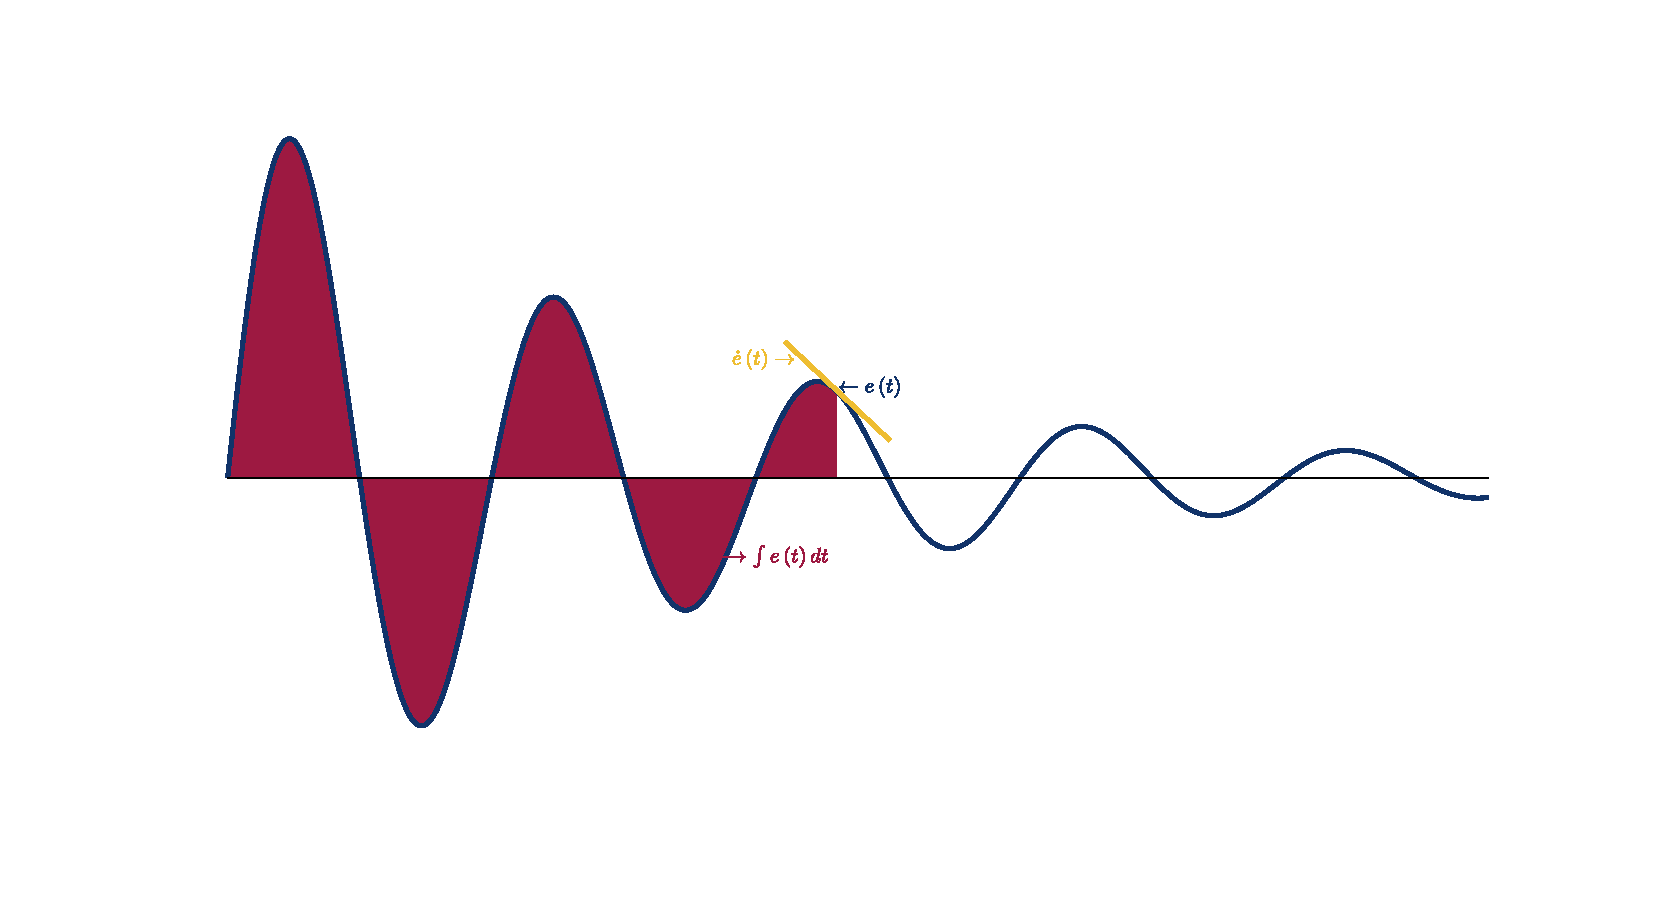
\includegraphics[width = 0.8\hsize]{pix/PIDSchematic.eps}
              \caption{Arbitrary error signal with a PID controller acting on it}\label{fig:PIDExp}
          \end{figure}

\end{itemize}
It is important to remember that when using  PID controllers, there will always be an element of
compromise within your system. For example, the ideal system will have a very low rise time, with
little to no steady state error or settling time, and no overshoot. However, this is very unrealistic in
the real world. If you were designing a highly precise robotic arm, you may need to tune your
controller in a way that there is practically no steady state error, but in order to do so, you will need to
have a higher rise time (i.e.\ the arm will move slowly, but it will go exactly where you need it). On
the other hand, you may have a system that requires a quick reaction time, for which you may need
to accept that there could be overshoot, or some steady state error.

You will also examine the concept of system types and their relation to PID controllers. Essentially,
systems can be type 0, 1, 2, etc \ldots A systems ``type'' determines its ability to track
the error on a given reference trajectory. For example, a system of type \(k \) can track
a reference trajectory with a bounded error for polynomials up to degree \(k \) (See Proposition
8.11 from the course notes for further clarification). We will see how the different terms from the PID controller transfer function affect the system type.

\section{Background Information}

\begin{itemize}
    \item \textcolor{blue}{TODO: Include some stuff from course notes?}
    \item \textcolor{blue}{TODO: Include simulink model rather than have them make it in procedure?}
    \item Learn the definitions for rise time, settling time, overshoot, steady-state value and steady state error.
    \item The closed loop transfer function of the system in \ref{fig:PID} is given by

          \begin{equation*}\label{eq:transfer}
              T(s)= \frac{R_{C}(s)R_{P}(s)}{1+R_{C}(s)R_{P}(s)}
          \end{equation*}

          where \( R_C = P + I\frac{1}{s} + Ds \) is the controller and \( R_P = \frac{\kappa_E}{s(s+\frac{1}{\tau})} \) is the plant. If using P, I, and D controls individually, the

    \item Determine the location of the closed loop poles when using P, I, D controls
          individually. What condition is required on the poles such that the system is BIBO stable?
\end{itemize}

\section{Procedure}

\begin{enumerate}
    \item Prepare a \textsf{Simulink} model to implement a PID controller as
          shown in Figure~\ref{fig:model6}\@. \emph{Modify your model from lab 1 or 2}.
          Figure~\ref{fig:model6}\@.
          \begin{figure}[htbp]
              \centering
              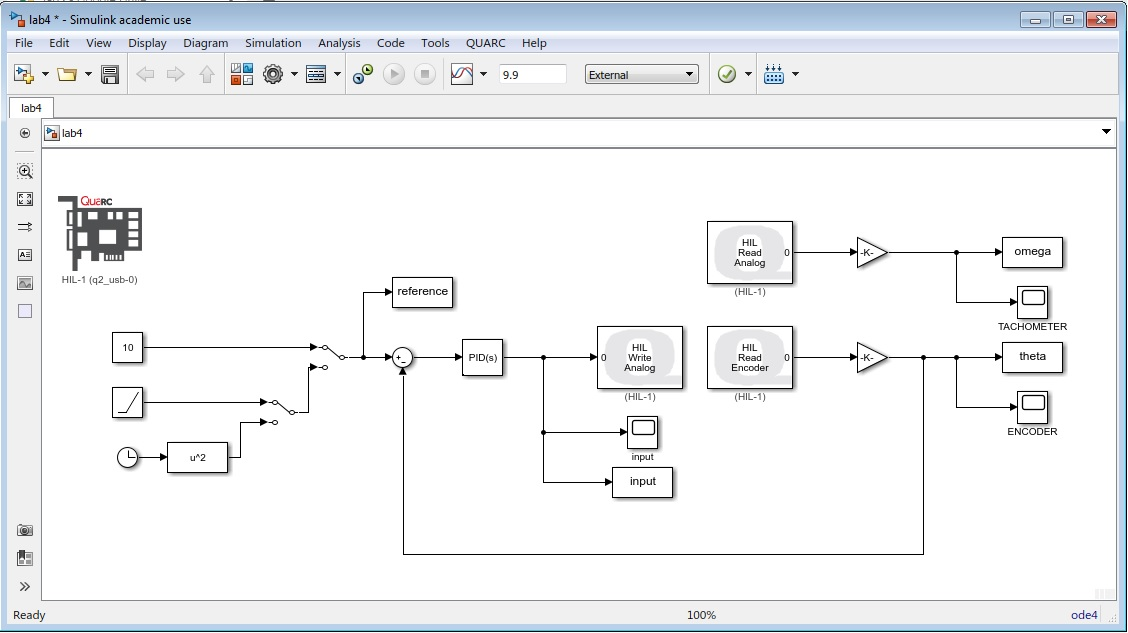
\includegraphics[width=0.6\hsize]{pix/performanceSpecificationModel4.jpg}
              \caption{\textsf{Simulink} model for a DC Servo Motor
                  system}\label{fig:model6}
          \end{figure}%
          The \verb|PID| block can be found in the \verb|Simulink| menu under the
          \verb|Continuous| section parameters.

          As shown in Figure~\ref{fig:PIDparameters}\@,
          \begin{figure}[htbp]
              \centering
              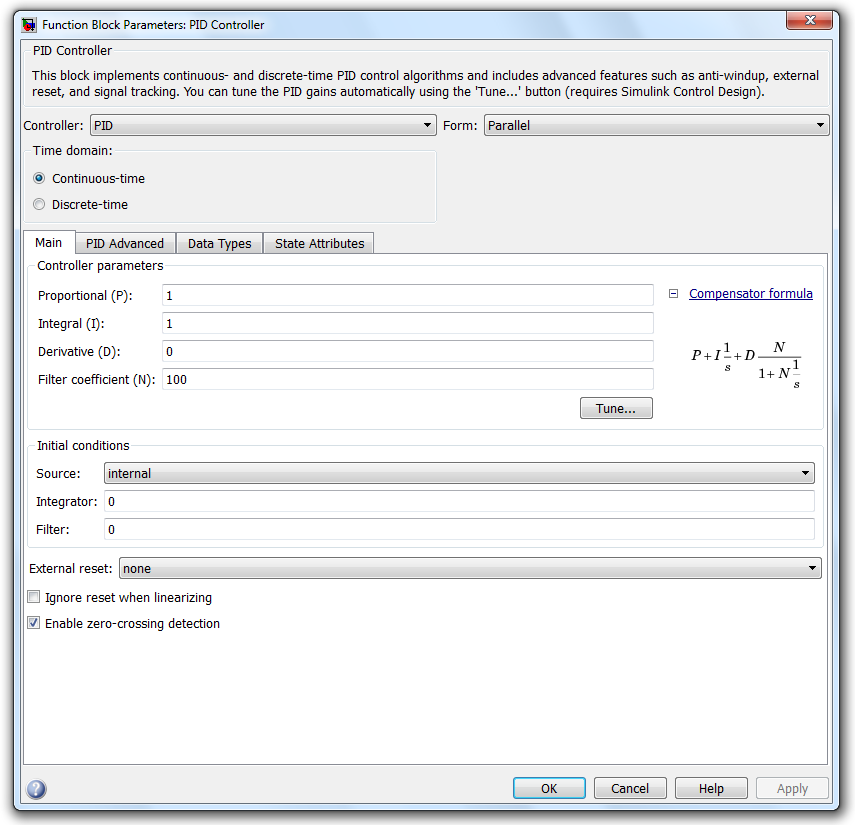
\includegraphics[width=0.6\hsize]{pix/PID.PNG}
              \caption{Screen shot of the \texttt{PID Controller} block}\label{fig:PIDparameters}
          \end{figure}%
          the \verb|PID| block contains three parameters: \(P\) is the proportional gain, of the controller; \(I\) is the integral action parameter which is equal; the \(D\) term provides the derivative action.
    \item\label{step:2} Set the desired angle to 10 radians.  The desired input is entered as
          shown in Figure~\ref{fig:model6} in the \verb|Constant| block. Remember to
          use the appropriate gain values from Table~\ref{tab:conversionFactors} for
          the encoder and tachometer to show results in radians.  Do not forget to
          change the \verb|solver| to \verb|ode 4| in \verb|Configuration Parameters|
          (\verb|Ctrl+E|).

    \item \textbf{Proportional Term}\label{step:3} \begin{enumerate}
              \item Build and run the \textsf{Simulink} model using only the
                    proportional term (i.e., set \(I\) and
                    \(D\) to zero). Comment on the effects of using various values of \(P\).
                    In particular, comment on the overshoot, rise time, settling time, and the
                    steady-state error for different values of \(P\), and be sure to tabulate this data (a table in Excel is an efficient way to do this). Use at least three different values of \(P\).

              \item Keep \(D\) and \(I\) at 0 and increase the value of \(P\) so the
                    system oscillates about the desired value of 10 radians without (seemingly)
                    decreasing in magnitude. Print a copy of the encoder output at that value, and a copy when using a slightly lower value of \(P\).

              \item Now reset your \(P\) value to the ``good'' value (i.e.\ not the value that makes
                    the system oscillate about 10 radians, but the value where you get a ``desirable'' response). Plot the error response of this system (i.e.\ the difference between input and output).
              \item Repeat the previous step but this time replace the constant input with linear input (i.e.\ disconnect the ``10'' block and connect the linear block). Plot the error response.
              \item Repeat the previous step but with the quadratic input (you may have to divide the quadratic term by 2 to prevent the encoder from going out of range).
              \item Based on the above error results, what is the type of the system when using only proportional control?
          \end{enumerate}

    \item \textbf{Derivative Term}\label{step:4} \begin{enumerate}
              \item Test various \(D\) values while keeping \(P\) constant (at the ``good'' value you found in the previous section), and comment on overshoot, rise time, settling time, and steady-state error. Again, tabulate this data, and decide on some ``good'' value of \(D\).
              \item Now, set \(P\) to 0 and repeat steps (c)-(e) from \ref{step:3} using only derivative control.
              \item Based on the above error results, what is the type of the system when using only derivative control?
          \end{enumerate}

    \item \textbf{Integral Term}\label{step:5} \begin{enumerate}
              \item Set your values of \(P\) and \(D\) to the values you found above, and test various \(I\) values.  Comment on the overshoot,
                    rise time, settling time, and steady-state error for these values of
                    \(I\), and tabulate the data.

              \item Now, set \(P\) and
                    \(D\) to zero and repeat steps (c)-(e) from \ref{step:3} using only integral control.
              \item Based on the above error results, what is the type of the system when using only integral control?
          \end{enumerate}

    \item Now we will consider a more complicated function input. To make things interesting, have the desired angle behave
          as four different functions on different intervals.  This can be achieved by
          preparing the \textsf{Simulink} model shown in Figure~\ref{fig:multiSwitch}\@.
          \emph{You do not need to use the exact same functions as shown in the figure}. Pick
          four functions that you think would be interesting.
          \begin{figure}[htbp]
              \centering
              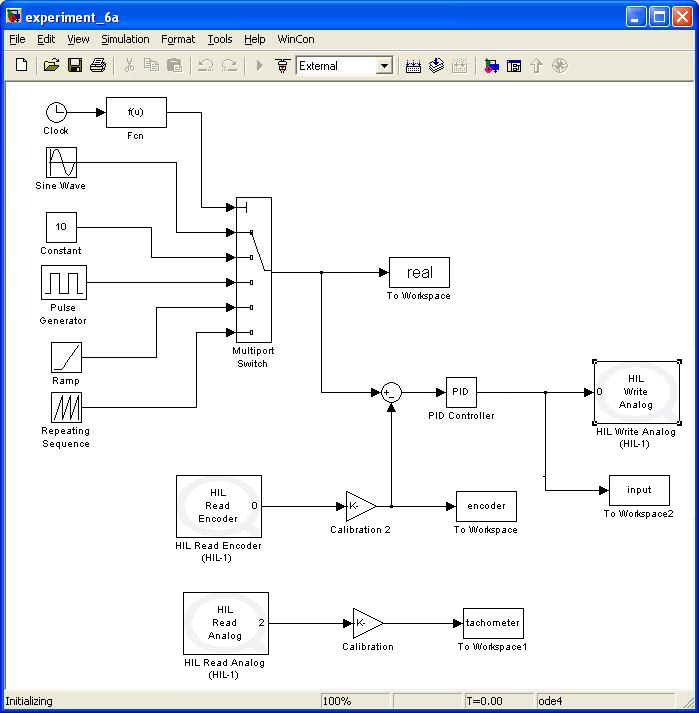
\includegraphics[width=0.6\hsize]{pix/lab6b.jpg}
              \caption{\textsf{Simulink} model for the implementation of multiple inputs and PID control}\label{fig:multiSwitch}
          \end{figure}%
          In this model, a number of possible sources have been introduced along with
          the switching logic.  The switching logic is based on the value of the
          function, \verb|4 sin(0.2*t)^{2}+1|.  This function, although arbitrary,
          assumes a value between 1 and 5 which is associated with ports 1 through 5 of
          the \verb|Multiport Switch| block.  The switching function is entered using
          the \verb|Fcn| block as indicated in Figure~\ref{fig:switchConfig}\@.
          \begin{figure}[htbp]
              \centering
              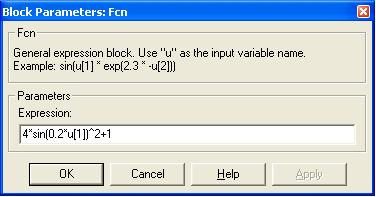
\includegraphics[width=0.6\hsize]{pix/fcnParameters.jpg}
              \caption{Configuration of the \texttt{Fcn} block for the implementation of multiple inputs and PID control}\label{fig:switchConfig}
          \end{figure}%

    \item Run the system and prepare a plot comparing the angle and the desired angle
          trajectory, making sure to note the values of the PID coefficients. You may have to tweak the PID values you found in previous sections in order to get a better trajectory.

          When you have completed the lab, make sure you save your files in the folder
          you created in Lab~\ref{chap:intro}\@.

\end{enumerate}

\section{Deliverables}

Prepare a brief write up describing what you learned from this lab. This does not
need to be a formal report, but all material should be presented in a clear and logical manner,
with concise descriptions where necessary. Include the following / answer the following questions:
\begin{enumerate}
    \item Include tabulated data of the response characteristics from steps~\ref{step:3}, \ref{step:4}, and~\ref{step:5}. Be sure that you are using your ``good'' \(P\) value (i.e. NOT the value that makes the system oscillate about 10 rad / s) when collecting data for \(I\) and \(D\) tests.
    \item Comment on how varying \(P\), \(I\), and \(D\) values impact response characteristics (i.e.\ rise time, settling time, etc\ldots).
    \item Include the plot of the output that oscillates consistently about the reference trajectory of 10 radians
          generated in step~\ref{step:3}. Why do higher \(P\) values increase the oscillation of the output? What is
          happening to the location of the closed loop poles in equation~\eqref{eq:transfer}?
    \item Include the plots of the error response when using only proportional, derivative, or integral control. Using your plots, what is the system type in each case? Is this consistent with the BIBO stability criteria in~\eqref{eq:transfer}?
    \item Include a plot of the output using your PID controller when the desired angle is generated by the multi-input
          switch. Be sure to specify your final P, I, and D values.
\end{enumerate}

%%% Local Variables: 
%%% mode: latex
%%% TeX-master: "lab-manual"
%%% End: 

%\chapter{Performance Specifications}

The purpose of this lab is to give you an understanding of the performance of
a second-order system.  In particular, you will be examining the effects that
system parameters have on various features of the output of that system.  In
the second part of the lab, you will examine the disturbance type of several
systems.

\section{Prelab}

Before you go into the lab, you should read the following:
\begin{itemize}
\item Sections 8.2.2, 8.2.3, and 8.3.1 in the course notes on performance specifications.
\item Be sure to familiarize yourself with the concept of system types. 
\end{itemize}
Then, determine the state space representation
$(\mat{A},\vect{b},\vect{c}^{t},\mat{D})$ of the generic second order model:
\begin{equation*}
\ddot y +2\zeta\omega_{0}\dot y+\omega_{0}^{2}y=\omega_{0}^{2}u.
\end{equation*}
Next, solve the above differential equation with a step response ($u = 1$), 
and comment on the effect of $\zeta$ and $\omega_0$, and how this relates to 
the location of the poles of your transfer function. 

\section{Key Concepts}

\begin{enumerate}
\item The main idea behind this lab is to understand how the addition of a zero 
affects the response of a system. For your system, let's say you add a zero at the 
point $\alpha$. What this will do to your governing equation is add a scaled derivative 
of the step response. The derivative of the step response (i.e. the impulse response)  
will be scaled by a factor of $\frac{\omega_0}{\alpha}$. Thus, for very large alpha, 
this term will have little impact on the systems response. However, if this zero exists 
very close to the imaginary axis, your system will have what is called undershoot.
\item Secondly, you must understand the definition of system types. Essentially, 
systems can be type 0, 1, 2, etc... A systems ``type" determines its ability to track 
the error on a given reference trajectory. For example, a system of type $k$ can track 
a reference trajectory with a bounded error for polynomials up to degree $k$. See Proposition 
8.11 from the course notes for further clarification. 


\end{enumerate}

\section{Procedure}

\subsection{Simulation of a second-order system}\label{subsec:simulation}

The model we will be examining is the generic second-order equation, where
the output of the system is position:
\begin{equation}\label{eq:sys}
\ddot y +2\zeta\omega_{0}\dot y+\omega_{0}^{2}y = \omega_{0}^{2}u.
\end{equation}
Since the physical constants of our friendly motor system cannot be changed
in the simple open-loop configuration, we are confined to the world of
simulations.  We will examine the behaviour of the second-order system in
\textsf{Simulink}.
\begin{enumerate}
\item Find the poles of your generic second-order system (or eigenvalues of your $\mat{A}$ matrix).
\item Open \textsf{Matlab} and build a \textsf{Simulink} model according to
Figure~\ref{fig:model7}\@.
\begin{figure}[htbp]
\centering
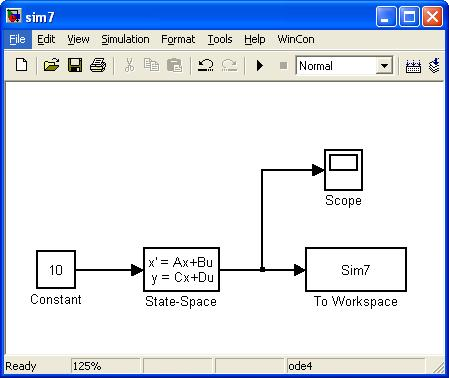
\includegraphics[width=0.6\hsize]{pix/model7.jpg}
\caption{\textsf{Simulink} model for a generic second-order system}\label{fig:model7}
\end{figure}%
You should have determined the values for
$(\mat{A},\vect{b},\vect{c}^{t},\mat{D})$ in your prelab. Define these matrices, in terms of $\zeta$ and $\omega_{0}$, in a script and simply call them in your model. We will use this model in section \ref{NMP}.

\item Run the system in simulation with initial values of $\zeta=0.5$ and
$\omega_{0}=1$\@. As this is a simulation, you do not need to build your system.

\item Using the \verb|step()| function in Matlab (and a \verb|for| loop), plot several values of $\zeta$ on the same graph using your $(\mat{A},\vect{b},\vect{c}^{t},\mat{D})$ matrices.
Print out the graph and write down your observations related to the response characteristics. It may be helpful to use different style of
lines for various values of $\zeta$. Details on plotting with various line
styles are discussed in Appendix~\ref{chap:MATLAB}\@.

\item Repeat the previous step with various values of $\omega_{0}$\@.
\end{enumerate}

\subsection{Non-minimum phase systems} \label{NMP}

The system described in Section~\ref{subsec:simulation} has the transfer
function
\begin{equation*}
T(s)=\frac{\omega_{0}^{2}}{s^{2}+2\zeta\omega_{0}s+\omega_{0}^{2}}.
\end{equation*}
We add a zero to the system as follows:
\begin{equation*}
T(s)=\frac{\hat y(s)}{\hat u(s)}=
\frac{\omega_{0}^{2}}{s^{2}+2\zeta\omega_{0}s+
\omega_{0}^{2}}\frac{(s+\alpha)}{\alpha}.
\end{equation*}
We use the parameter $\alpha$ to vary the position of the zero.  In
particular, we can use it to place our zero in $\mathbb{R}_{<0}$ or
$\mathbb{R}_{>0}$\@.  Notice that we have $\alpha$ in the denominator as
well.  This is a done to normalize the system at $s=0$\@.

To convert this back into the time domain, we simply cross-multiply the
transfer function to get the state equation
\begin{equation*}
\ddot y +2\zeta\omega_{0}\dot y+\omega_{0}^{2}y =
\frac{\omega_{0}^{2}}{\alpha}\dot u+\omega_{0}^{2}u.
\end{equation*}
You can see that the only difference is that we now have a term involving
$\dot u$.  Since $u$ is a step function, $\dot u$ is going to be an impulse
function.\footnote{The derivative here is understood in the sense of
distributions.}  Implementing an impulse function cannot be done directly,
but we can side-step the problem by cooking the initial conditions so that
our initial value problem is a solution to our system when given a step
input.  It turns out that these initial conditions are $y(0)=0$, and $\dot
y(0)=\frac{\omega_{0}^{2}}{\alpha}$\@.\footnote{This is a little involved,
but see Section 3.6.5 of the course text for
details.}
\begin{enumerate}
\item Modify the model from the previous section to incorporate the zero
added to the system by adding the initial conditions. The way to enter
initial conditions into the model is shown in
Lab~\ref{chap:controlandobserve}\@.

\item For $\alpha = \left\{0.1, 1, 10\right\}$, what is the effect of increasing
$\alpha$ on the rise time, settling time, overshoot, and peak
time?  Using \textsf{Matlab}, plot the output of these positive
$\alpha$ values and print the graph.  On the graph, write down your
discoveries. \label{step1}

\item For $\alpha = \left\{-0.1, -1, -10\right\}$, what is the effect of increasing the
magnitude of $\alpha$ on the rise time, settling time, overshoot,
and peak time? Using \textsf{Matlab}, plot the output of these negative $\alpha$ values and print the graph.  On the graph, write down
your discoveries.  What is the most noticeable characteristic of a
non-minimum phase system?  \label{step2}
\item\label{step:superposition} Lastly, we will be observing exactly what the addition of a zero does 
to the system. 
\begin{enumerate}
\item In Matlab, plot the step response and impulse response of your 
original system (without the zero) shown in equation~\ref{eq:sys} using the \verb|step| and 
\verb|impulse| commands. 
\item \label{step3} On a separate graph, plot the addition of the step response with 
the impulse response scaled by a factor of $\frac{\omega_0^2}{\alpha}$ (use the same $\alpha$ values from above). Note: only the impulse response should be scaled. When using the 
\verb|step| and \verb|impulse| commands, you must ensure that the arrays have the same length in 
order to superimpose them. This may involve truncating one array to match the length of the other. 
\item Comment on your plots obtained in part \ref{step3} with those obtained in step \ref{step1} and \ref{step2}. Hint: The plots should be the exact same. Comment on why that is.
\end{enumerate}
\end{enumerate}

\subsection{System type}

We will now examine three different motor system and the system type of each
one.  The basic configuration is shown in
Figure~\ref{fig:feebackWithDisturbance}\@.
\begin{figure}[htbp]
\centering
\begin{picture}(240,75)
\put(0,50){\(\hat\theta_{d}(s)\)}
\put(20,53){\vector(1,0){15}}
\put(40,53){\circle{7}}
\put(45,53){\vector(1,0){15}}
\put(63,37){\framebox(35,33){$R_{C}(s)$}}
\put(100,53){\vector(1,0){20}}
\put(123,37){\framebox(80,33){$R_{P}(s)=\frac{k_{E}}{s(s+\frac{1}{\tau})}$}}
\put(205,53){\vector(1,0){30}}
\put(237,50){$\hat\theta(s)$}
\put(215,53){\line(0,-1){45}}
\put(215,8){\line(-1,0){175}}
\put(40,8){\vector(0,1){40}}
\put(30,48){\line (1,0) {4}}
\end{picture}
\caption{Feedback system with disturbance}\label{fig:feebackWithDisturbance}
\end{figure}%
This is an interconnected system, but we will take a ``black box'' approach,
applying the disturbance at the input node, and measuring at the output node.
Recall that the motor is modelled by transfer function
$\frac{k_{E}}{s(s+\frac{1}{\tau})}$ when the output is the motor angle
$\theta$\@.
\begin{enumerate}
\item System 1 has the controller transfer function $R_{C}(s)=5$\@.
Verify by hand that the transfer function
\begin{equation*}
T(s)= \frac{R_{C}(s)R_{P}(s)}{1+R_{C}(s)R_{P}(s)}
\end{equation*}
is BIBO stable. Hint: What is $R_{C} = 5$ equivalent to? What do we know about this from lab 3?

\item Determine the system type for this particular system.

\item Assemble (or modify an existing) a \textsf{Simulink} model according to
Figure~\ref{fig:model7a}\@.
\begin{figure}[htbp]
\centering
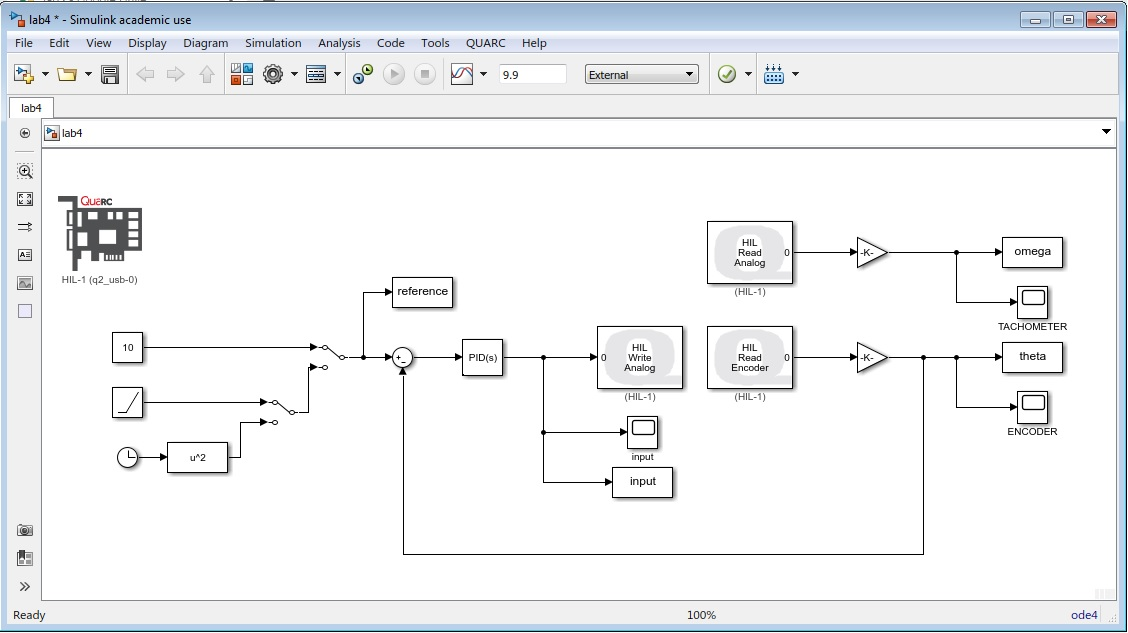
\includegraphics[width=0.6\hsize]{pix/performanceSpecificationModel4.jpg}
\caption{\textsf{Simulink} model for a DC Servo Motor
system}\label{fig:model7a}
\end{figure}%

\item Run the system using the constant input.  What is the steady-state
error of the system?  Plot the error response in \textsf{Matlab} and print a
copy of the plot with appropriate titles and axis labels. Is this consistent
with your earlier work?

\item Repeat the above step, but use a linear and quadratic term (divide the quadratic term by 2 to ensure the encoder does not go out of range) for the
reference signal.  Plot all the error responses and make print outs.  Make
sure you have proper axis labels and titles.

\item System 2 has the same plant transfer function and a new
controller transfer function given by $R_{C}(s)=\frac{1}{s}$\@.  Is this
system BIBO stable?  If so, what is the system type?

\item Make changes to the system to implement the new controller and run the
system with a constant, a linear, and a quadratic reference signal.  Are the
results consistent with your answer from above?

\item System 3 has the same plant transfer function and a new
controller transfer function given by $R_{C}(s)=s$\@.  Is this system BIBO
stable?  If so, what is the system type?

\item Make changes to the system to implement the new controller and run the
system with a constant, a linear, and a quadratic reference signal.  Are the
results consistent with your answer from above? 

\item Plot all the error responses in \textsf{Matlab} graph and print them.
Make sure you have proper axis labels and titles.
\end{enumerate}

When you have completed the lab, make sure you save your files in the folder
you created in Lab~\ref{chap:intro}\@.

\section{Deliverables}

Prepare a brief write up describing what you learned from this lab. This does not
need to be a formal report, but all material should be presented in a clear and logical manner,
with concise descriptions where necessary. Include the following/Answer the following questions:
\begin{enumerate}
\item Include plots of the systems response with varying $\zeta$ and $\omega_0$ values, comment 
on the effect off varying these constants. 
\item For both positive and negative $\alpha$ values, what is the effect of increasing the magnitude 
of $\alpha$ on the rise time, settling time, overshoot/undershoot, and peak time? Include plots. 
\item In step~\ref{step:superposition} of the non-minimum phase system section, explain why your two 
plots are the same. 
\item Create the following table for the system type section. Be sure to include and reference all 
necessary plots for the justification section. 
\begin{table}[htbp]\label{tab:systype}
\centering
\begin{tabular}{|c|p{2.5cm}|p{2.5cm}|p{2.5cm}|c|c|}\hline
System No.&Response to Constant Input&Response to Ramp Input&Response to Quadratic Input&
Type?&Justification\\\hline
System 1&&&&&\\\hline
System 2&&&&&\\\hline
System 3&&&&&\\
\hline
\end{tabular}
\end{table}%
\end{enumerate}

%%% Local Variables: 
%%% mode: latex
%%% TeX-master: "lab-manual"
%%% End: 

%\chapter{The Nyquist criterion}

In this lab, you will use the Nyquist contour to determine if a system is
IBIBO stable.  The Nyquist plot is a conformal mapping of a closed loop in
complex plane and it is a tool for the understanding of the stability of a
closed-looped system.  Furthermore, you will be examining the relationship
between the Nyquist contour and the Bode plot, thus familiarizing yourself
with such terms as \emph{crossover frequency}\@, \emph{gain margin}\@, and
\emph{phase margin}\@.

\section{Background Info}
\textcolor{blue}{This references the Bode plots from 393, should we include Bode plots here?}

\section{Procedure}

\subsection{Using the Bode plot to sketch the Nyquist
    contour}\label{sec:bodeNyquist}

For this part of the lab, we will be using the motor in the unity gain
feedback configuration shown in Figure~\ref{fig:generic}\@.
\begin{figure}[htbp]
    \centering
    \begin{picture}(230,75)
        \put(0,50){\(\hat\theta_{d}(s)\)}
        \put(25,53){\vector(1,0){15}}
        \put(45,53){\circle{7}}
        \put(32,57){+}
        \put(50,53){\vector(1,0){20}}
        \put(73,37){\framebox(35,33){\(R_{C}(s)\)}}
        \put(110,53){\vector(1,0){40}}
        \put(152,37){\framebox(35,33){\(R_{P}(s)\)}}
        \put(190,53){\vector(1,0){30}}
        \put(224,50){\(\hat\theta(s)\)}
        \put(206,53){\line(0,-1){45}}
        \put(205,8){\line(-1,0){160}}
        \put(45,8){\vector(0,1){40}}
        \put(35,48){\line (1,0) {4}}
    \end{picture}
    \caption{Feedback system with disturbance}\label{fig:generic}
\end{figure}%
This setup should be quite familiar to you by now, so you should have a
well-developed intuition concerning the IBIBO stability of such a system.  We
will be taking the output of the system to be the motor velocity, \(\omega \),
so our plant transfer function is \(R_{P}(s)=\frac{k_{E}}{s+\frac{1}{\tau}}\).
In Lab 2 you constructed the Bode plot for this system
experimentally.
\begin{enumerate}
    \item Using the Bode plot from Lab 2, determine the gain
          and phase crossover frequencies, and the phase and gain margins at these
          frequencies; see Section 7.2.2 from the course text.

    \item Using the Bode plot determine the general transfer function, from the
          transfer function sketch the corresponding Nyquist contour.  Looking also at
          the transfer function, determine whether or not the system is IBIBO stable.

    \item Start up \textsf{Matlab} and define \verb|t| to be the transfer
          function of the open-loop motor scheme.  Essentially, we are just setting
          \(R_{C}(s)=1\) to see how motor behaves on its own.

    \item To plot the Nyquist contour, use the \verb|Nyquist| command in
          \textsf{Matlab}.

    \item Is the Nyquist contour consistent with what you know about the IBIBO
          stability of the system?  Comment on both the poles of the transfer function,
          and the zeroes of the characteristic polynomial.
\end{enumerate}

\subsection{Using a proportional controller}

We will now turn our attention to the task of using the Nyquist contour as a
tool in determining what range of values of a proportional controller can
take on in order to make the system IBIBO stable.

The plant transfer function \(R_{C}(s) = K\) will be used in the feedback
configuration depicted in Figure~\ref{fig:generic}\@.  The transfer function
for this system is simply
\begin{equation*}
    T(s)=\frac{KR_{P}(s)}{1+KR_{P}(s)}.
\end{equation*}
What is important to note is that the condition \(KR_{P}(s)=-1\) is equivalent
to the condition \(R_{P}=-\frac{1}{K}\). This seems obvious in itself, but what
this allows you to do is to use the Nyquist contour for \(R_{P}(s)\) on its own
(i.e., with \(K=1\)), and determine where you would like the point
\(\frac{1}{K}\) to be. This allows you to get a lot of mileage out of only one
plot. The alternative is to construct the Nyquist contour for many values of
\(K\), and see if each contour has the required number of encirclements of the
point \(-1+\imag0\).  This may not seem like a bad alternative if you have
access to a computer, but the method of normalizing the proportional gain is
much more efficient.

\begin{enumerate}
    \item In \textsf{Matlab}, define the plant transfer function to be
          \(R_{P}=\frac{s+1}{s(\frac{s}{10}-1)}\).

    \item Produce both the Bode plot and the Nyquist contour.  Take a minute to
          further reaffirm your faith in the relationship between the two.

    \item What are the crossover frequencies, and what are the gain and phase
          margins at these frequencies?

    \item Since our plant transfer function has one pole in the right-half
          complex plane, we require one counterclockwise encirclements of the point
          \(\frac{1}{K}\). Using this information, in which region should we place the
          point \(-\frac{1}{K}\)?

    \item What values of \(K\) satisfy the above requirement?

    \item Repeat the above procedure for the plant transfer function
          \(R_{P}(s)=\frac{1}{s{(s+1)}^{2}}\).  Remember, Nyquist plots always close
          clockwise.
\end{enumerate}

\subsection{The phase margin}

In this part of the lab we will quickly demonstrate the phase margin as it
applies to the Nyquist contour.
\begin{enumerate}
    \item We will use the plant transfer function
          \(R_{P}(s)=\frac{1}{s{(s+1)}^{2}}\).  Produce the Bode plot and the Nyquist
          contour of this system.

    \item Determine how much you have to boost the gain (in decibels) to provide
          a phase margin of \(0^{\circ}\) at a gain cross over frequency of
          \(10^{n}\frac{\textup{rad}}{\textup{sec}}\), \(n\in\mathbb{Z}\).  Will the %chktex 35
          resulting system, with this gain boosted by using a proportional controller,
          be IBIBO stable?

    \item The number you get is a scalar that represents the factor by which you
          can ``stretch'' (or ``shrink'' as the case may be) the Nyquist contour
          towards the point \(-1+\imag0\) and still maintain IBIBO stability (assuming
          the system is stable for \(K=1\), which our system is).  Looking at the Nyquist
          contour, does this scalar quantity seem to make sense?  Is this consistent
          with your work from Section~\ref{sec:bodeNyquist}?
\end{enumerate}

When you have completed the lab, make sure you save your files in the folder
you created in Lab~\ref{chap:intro}\@.

%%% Local Variables: 
%%% mode: latex
%%% TeX-master: "lab-manual"
%%% End: 

%\chapter{PID design using frequency response}

In this lab, you will use the Bode plot you produced using the measurements
for the motor to design a PID controller to meet specified performance
criteria.

\section{Prelab}

Before you go into the lab, you should read the following:
\begin{itemize}
    \item Section 12.2 from the course text on using
          frequency response method for controller design.
\end{itemize}
Since \textsf{Simulink} does not allow improper transfer functions, you must
use the \verb|PID| block for the controller in this lab.  Find the
relationships between the constants in equation~\eqref{eqn:con1}
and~\eqref{eqn:con2}\@:
\begin{gather}\label{eqn:con1}
    \frac{K}{s}(1+T_{D}s)(s+\frac{1}{T_{I}}),\\\label{eqn:con2}
    P+\frac{I}{s}+Ds.
\end{gather}

\section{Procedure}

Before we implement the controller, we need to do some paper work to design
it.

\subsection{Design specifications}

You are charged with the designing the controller rational function \(R_{C}\)
in the feed back loop in Figure~\ref{fig:PIDfeedback}\@.
\begin{figure}[htbp]
    \centering
    \begin{picture}(230,75)
        \put(0,50){\(\hat u(s)\)}
        \put(20,53){\vector(1,0){15}}
        \put(40,53){\circle{7}}
        \put(28,57){+}
        \put(45,53){\vector(1,0){20}}
        \put(68,37){\framebox(35,33){\normalsize \(R_{C}(s)\)}}%-50 in width
        \put(105,53){\vector(1,0){40}}
        \put(147,37){\framebox(35,33){\normalsize \(R_{P}(s)\)}}
        \put(185,53){\vector(1,0){30}}
        \put(217,50){\(\hat y(s)\)}
        \put(201,53){\line(0,-1){45}}
        \put(201,8){\line(-1,0){161}}
        \put(40,8){\vector(0,1){40}}
        \put(30,48){\line (1,0) {4}}
    \end{picture}
    \caption{Feedback system with disturbance}\label{fig:PIDfeedback}
\end{figure}%
The plant transfer function is that for the motor:
\begin{equation*}
    R_{P}(s)=\frac{k_{E}}{s(s+\frac{1}{\tau})},
\end{equation*}
where you have measured the values for \(k_{E}\) and \(\tau \) in Lab~\ref{chap:intro}\@.

You are asked to design a controller so that the closed-loop system has a
phase margin of \(65^{\circ}\) and a crossover frequency as large as possible.
The controller you will use is a PID controller in the form
\begin{equation*}
    R_{C}(s)=\frac{K}{s}(1+T_{D}s)(s+\frac{1}{T_{I}})=
    K(1+\frac{T_{D}}{T_{I}}+T_{D}s+\frac{1}{T_{I}s}).
\end{equation*}

\subsection{The steps in controller design}

We shall lead you by hand through the design process.
\begin{enumerate}
    \item Produce the Bode plot for plant transfer function using
          \textsf{Matlab}.

    \item In the PID controller design, let us decide to fix \(T_{I}=10T_{D}\).
          You are free to change this ratio during the lab if you find it unsuitable.

    \item Also, to start the design process, let us fix the gain \(K\) to 1.  You
          may want to use the \verb|zpk| function in \textsf{Matlab} to define the
          transfer function.

    \item With the above assumptions, is it true that there is a choice for
          \(T_{D}\) for which the closed loop system is IBIBO stable (IBIBO stability can
          be verified either by Nyquist Criterion or Hurwitz Criterion)?  Is it true
          that, no matter what choice one makes for \(T_{D}\), the closed-loop system
          will be IBIBO stable?  Can you spot the features on your Bode and/or Nyquist
          plot which help you answer this question?  How do these play a role in the
          design of the controller?

    \item Based upon the considerations in the previous step, choose a value for
          \(T_{D}\) which meets the design objectives.

    \item Now choose \(K\) to give the crossover frequency.

    \item Make sure the closed-loop system is IBIBO stable using the Nyquist
          criterion.
\end{enumerate}

You now have values for \(K\), \(T_{D}\), and \(T_{I}\) which you will carry
into the rest of the procedure.

\subsection{Executing the design in hardware/software}

Now you will implement your controller in hardware.
\begin{enumerate}
    \item Open \textsf{Matlab} and build a \textsf{Simulink} model according to
          Figure~\ref{fig:model9a}\@.
          \begin{figure}[htbp]
              \centering
              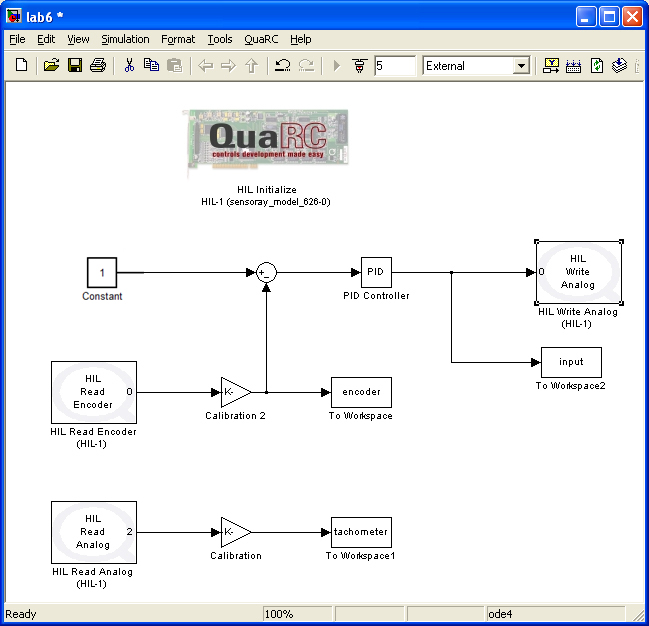
\includegraphics[width=0.6\hsize]{pix/lab9a.jpg}
              \caption{\textsf{Simulink} model for the implementation of PID control using
                  frequency response method; step reference}\label{fig:model9a}
          \end{figure}%

    \item Use values for \(K\), \(T_D\), and \(T_I\) that make the closed loop
          system unstable in hardware.  Use the above contraints you just calculated to
          determine values that cause instability.  Be prepare to shut the system off!
          Produce plots of the unstable system.

    \item Now, using an input step response of \(1\), use the ``good'' values for
          \(K\), \(T_D\), and \(T_I\) to determine the rise time, the percentage
          overshoot, and the \(\epsilon \)-settling time for \(\epsilon=0.5\).

    \item Now run the system with your ``good'' values for \(K\), \(T_D\), and
          \(T_I\) and a sinusoidal input whose magnitude is \(1\) and whose frequency is
          the crossover frequency that was calculated above; see
          Figure~\ref{fig:model9} for the \textsf{Simulink}\@.
          \begin{figure}[htbp]
              \centering
              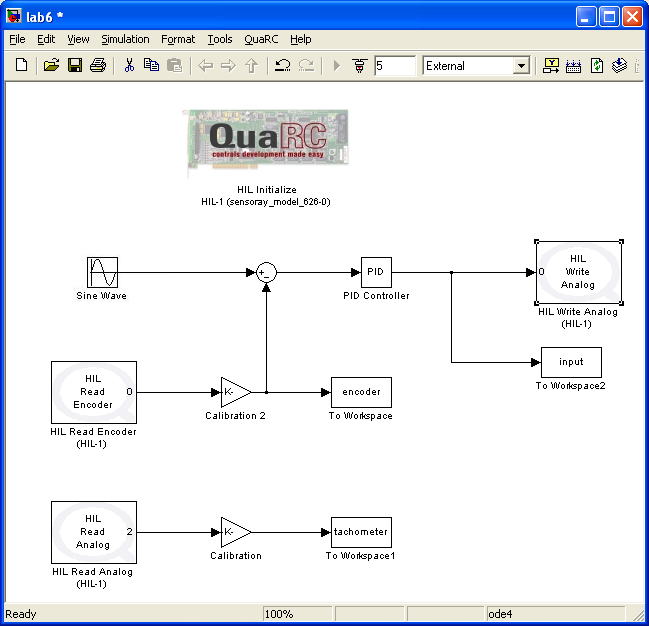
\includegraphics[width=0.6\hsize]{pix/lab9.jpg}
              \caption{\textsf{Simulink} model for the implementation of PID control using
                  frequency response method; sinusoidal reference}\label{fig:model9}
          \end{figure}%
          What is the magnitude of the output compared to the input, and what is the
          phase of the output relative to the input?

    \item Is your controller a good one?  How might you improve it?  What do your
          improvements mean in terms of loopshaping ideas?

    \item Change the ratio of \(\frac{T_{I}}{T_{D}}\) and discuss the effect on the
          performance of the controller.  Does what you observe make sense?  Generate
          plots to demonstrate your observations.
\end{enumerate}

When you have completed the lab, make sure you save your files in the folder
you created in Lab~\ref{chap:intro}\@.

%%% Local Variables: 
%%% mode: latex
%%% TeX-master: "lab-manual"
%%% End: 

\chapter{Controllability and observability}\label{chap:controlandobserve}

This lab will demonstrate the fundamental ideas behind the controllability
and observability properties of a system.  You will analyze a simple circuit
and determine the conditions for observability and controllability.  You will
then proceed to simulate the system using \textsf{Simulink} under various
conditions.

\section{Prelab}

You may wish to read Sections 2.3.1 and 2.3.2 from the
course notes to recall some background on controllability and observability.

Using Figure~\ref{fig:circuit}
\begin{figure}[htbp]
    \centering
    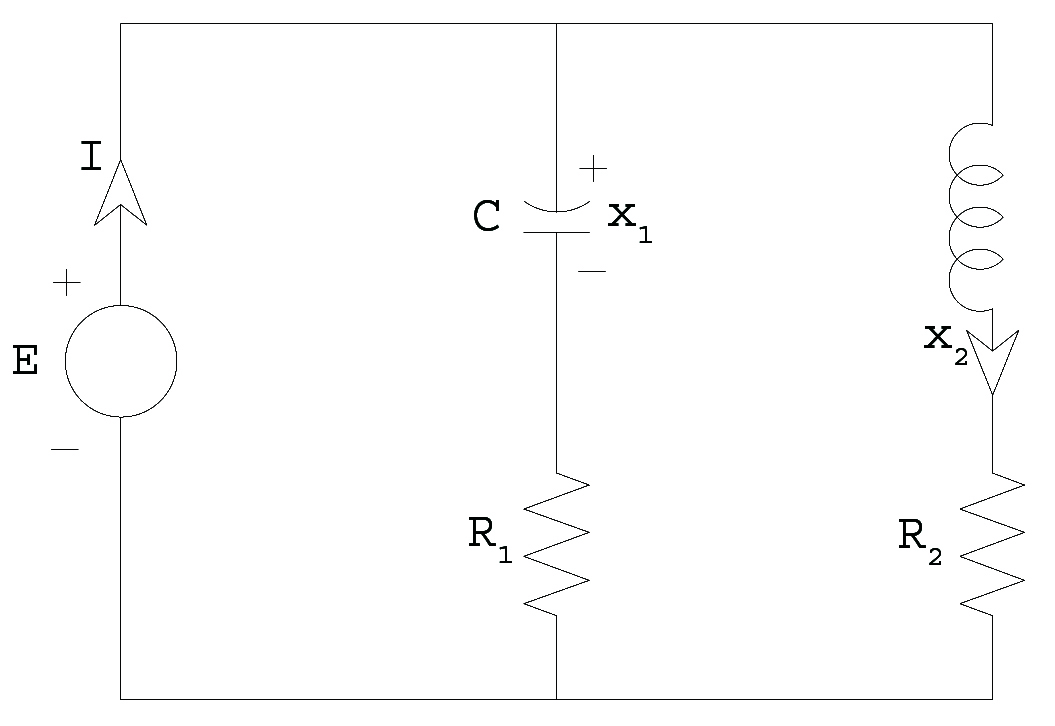
\includegraphics[width=0.6\hsize]{pix/circuitlarge.jpg}
    \caption{State space configuration}\label{fig:circuit}
\end{figure}
as a reference, define \(x_{1}\) as the voltage across the capacitor, and
\(x_{2}\) as the current through the inductor.  Take the output to be the
current entering the circuit, denoted \(I\) in Figure~\ref{fig:circuit}.

\begin{enumerate}
    \item Write out the system equations in the state-space form:
          \begin{eqnarray*}
              \dot{\vect{x}}=\mat{A}\vect{x}+\vect{b}u,\\y=\vect{c}^{t}+\mat{D}u.
          \end{eqnarray*}
          If you are having trouble getting the differential equations, or just not
          ``electrically inclined'', you should review past course notes on electrical
          circuits and differential equations.  Suck it up, Apple Mech students!
          \begin{itemize}
              \item When finding the differential equations for a system, your goal should
                    be to determine an expression for the derivative of each state variable in
                    terms of the state variable(s) and the forcing function.  Once you have %chktex 36
                    these, you can determine \(\mat{A}\) and \(\vect{b}\).

              \item The following facts may be useful.  The current through a capacitor is
                    given by \(I_{c}=C\frac{dV_{C}}{dt}\), the voltage across an inductor is
                    given by \(V_{L}=L\frac{dI_{L}}{dt}\), and the voltage across a resistor is
                    given by Ohm's law, \(V_{R}=I_{R}R\).  By Kirchoff's voltage law, the voltage
                    across each branch of the circuit is simply \(E\). You can use this fact to
                    get expressions for \(\mat{A}\) and \(\vect{b}\).

              \item Since the output is the current entering the circuit, and you will by
                    this point have expressions available for the current in each branch, you can
                    use Kirchoff's current law (i.e., conservation of current) to determine
                    expressions for \(\vect{c}\) and \(\mat{D}\).
          \end{itemize}

    \item Calculate the controllability matrix \(\mat{C}(\mat{A},\vect{b})\).

    \item Calculate the observability matrix \(\mat{O}(\mat{A},\vect{c})\).

    \item Determine the conditions under which the system is uncontrollable.
          Recall that a square matrix has full rank if and only if its determinant is
          non-zero.

    \item Determine the conditions under which the system is unobservable.

    \item When the system is uncontrollable, determine the set of reachable
          points for zero initial conditions.  This is going to be a one-dimensional
          vector space, so there is a simple relationship between \(x_{1}\) and \(x_{2}$.
          Determine this relationship when the system is uncontrollable.

    \item When the system is unobservable, determine the set of initial
          conditions that yield the same output, and the linear relationship between
          the initial conditions.
\end{enumerate}

\section{Procedure}

Via simulation, you will determine the conditions under which the circuit in
Figure~\ref{fig:circuit} is controllable and/or observable.

\subsection{Controllability}

When analyzing the controllability, you will be examining the behaviour of
the system states.  Recall that a rough definition of controllability is:
``starting from the origin, you can reach any point in state space by
applying an appropriate input.''
\begin{enumerate}
    \item Build the \textsf{Simulink} model as shown in
          Figure~\ref{fig:model2}.
          \begin{figure}[htbp]
              \centering
              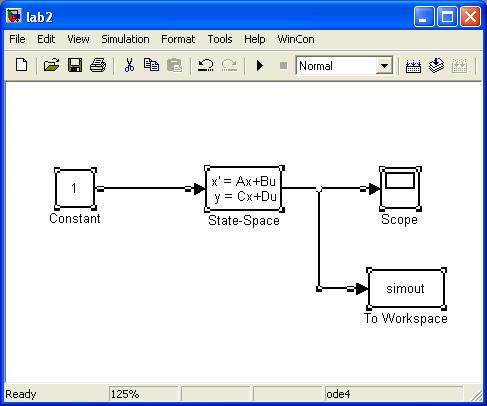
\includegraphics[width=0.6\hsize]{pix/controlandobservemodel.jpg}
              \caption{\textsf{Simulink} model for Lab~\ref{chap:controlandobserve}}\label{fig:model2}
          \end{figure}%
          The model applies a constant voltage to the dynamic model defined by
          \(\mat{A}\), \(\vect{b}\), \(\vect{c}\), and \(\mat{D}\) defined
          previously. The output is the current in the circuit.

    \item Define the matrices \(\mat{A}$\@, \(\vect{b}$\@, \(\vect{c}\), and
          \(\mat{D}\) by double-clicking on the \verb|State-space| block.  Each matrix is
          entered using the following convention. The following is an example on how to
          properly input values into the \verb|State-Space| block. The values shown are
          \emph{not} the proper values.  Use values that correspond to the matrices in
          the prelab.  The matrix
          \begin{equation*}
              \mat{A}=\begin{bmatrix}0&1\\-1&2\end{bmatrix}
          \end{equation*}
          is entered by typing \verb|[0,1;-1,-2]| in the line reserved for \(\mat{A}$\@.
              Note that elements of a row are delimited by comma (or spaces) and each row
              is delimited by a semicolon.

              The entries of Figure~\ref{fig:stateConfiguration}
              \begin{figure}[htbp]
                  \centering
                  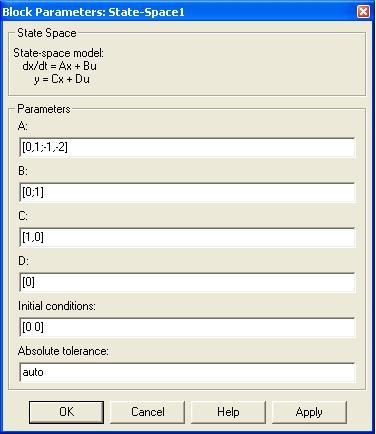
\includegraphics[width=0.6\hsize]{pix/controlandobserveentries.jpg}
                  \caption{State space configuration}\label{fig:stateConfiguration}
              \end{figure}%
              correspond to the dynamical system
              \begin{eqnarray*}
                  \dot{\vect{x}}&=&\begin{bmatrix}0&1\\-1&-2\end{bmatrix}\vect{x}
                  +\begin{bmatrix}0\\1\end{bmatrix}u,\\
                  y&=&\begin{bmatrix}1&0\end{bmatrix}\vect{x}+[0]u.
              \end{eqnarray*}
              Note that the last line specifies the initial conditions for the states.  In
              this case, we have set \(x_{1}(0)=0\) and \(x_{2}(0)=0$\@.  Come up with an
          appropriate variable to show the linear relationship between \(x_{1}\) and
          \(x_{2}\) when the system is uncontrollable (make sure you record this in your
          lab report).  Define this variable as one of your outputs in your model.
          Note that you can add as many outputs as you want just by adding rows to the
          matrix \(\vect{c}$\@.

          Define the initial conditions to be zero.  The default final time is set to
          10 by \textsf{Simulink}.  You may change it by opening the window
          \begin{center}
              \verb|Simulation|\(\rightarrow \)\verb|Configuration Parameters|
          \end{center}
          and entering the required time in the \verb|Stop Time| box.

    \item Run the \textsf{Simulink} block under uncontrollable conditions. This
          will depend on your choice of \(R_{1}\), \(R_{2}\), \(C\), and \(L\).
          Recuperate the state variable values written to the workspace and plot
          \(x_{1}\), \(x_{2}\), and the output variable you defined.  Does the output
          variable you chose show that there is, in fact, a linear relationship between
          \(x_{1}\) and \(x_{2}\)? Under these conditions, is it possible to find an input
          voltage \(E\) that will allow you to reach a point that is off this line?

    \item Add an appropriate title to your graph and print it.

    \item Rerun the system, but this time use conditions that make the system
          controllable.  Plot and print a graph of \(x_{1}\) and \(x_{2}\) and your output
          variable.  What can you now say about your output variable?  What is the set
          of reachable points under these conditions?

    \item Again, give an appropriate title to your graph and print it.
\end{enumerate}

\subsection{Observability}

When analyzing observability, you will be examining the output behaviour of
the system.  Recall that a rough definition of observability is: ``a change
in initial conditions and/or input results in a change in the output.''
\begin{enumerate}
    \item Using the work from your prelab, enter the value of \(\mat{A}\),
          \(\vect{b}\), \(\vect{c}\), and \(\mat{D}\) into the \verb|State-Space| block.
          Change the name of the output variable from \verb|simout| to \verb|I|.

    \item We will want to examine the output using many different initial
          conditions.  Build and run the system using a pair of initial conditions that
          are in the kernel of the observability matrix.  Plot, and print a graph of
          the output variable \(I$.  Make sure that you include values of the constants
          in the title of the plot.

    \item Rerun the system using a different pair of initial conditions that are
          also in the kernel of the observability matrix.  Include a plot of the
          output.  Does the result of this experiment confirm your work from the
          prelab? What happens if you use initial conditions that are not in the kernel
          of the observability matrix?
\end{enumerate}

When you have completed the lab, make sure you move the files created in the
directory created in Lab~\ref{chap:intro}.

%%% Local Variables: 
%%% mode: latex
%%% TeX-master: "lab-manual"
%%% End: 

\chapter{Stability, Feedback Control \& Luenberger Observer for Balancing an Inverted Rotary Pendulum}

The purpose of this lab is to study the rotary pendulum system and to develop a control technique that balances the pendulum around an equilibrium using partial state feedback and a linear observer. In the lab, you will first use full state feedback and pole placement techniques to develop a controller that balances the inverted pendulum. Then, you will carry out the same task for the case where you do not have access to the full state information. To do this, you will develop a Luenberger observer to estimate the states that you do not have access to and you will use the estimated states to develop a controller that balances the inverted pendulum.
\begin{figure}[htb!]
    \centering
    \includegraphics[width=.3\linewidth]{eps/lab_3/quanser.eps}
    \caption{Qanser SRV02 with pendulum module, shown in an inverted orientation~\cite{Q-Flex-Beam}.}
    \label{fig:lab3_plant}
\end{figure}

\section{Background Information}
\subsection{Modelling the Pendulum Using the Euler-Lagrange Equation}
From previous mechanics courses, you should be familiar with modelling physical systems using first principles (i.e., Newton's Laws). For simple systems, this first principles approach to modelling a physical system is relatively straightforward and works very well; however, for more complicated systems, things can get ugly very quickly. For modelling our rotary flexible beam, it is easier to use a more modern approach to modelling that employs the \emph{Euler-Lagrange equation}.

The Euler-Lagrange equation is a second-order partial differential equation that will help you find the equations of motion for our physical system. Those interested in the specifics of the Euler-Lagrange equation and related calculations can find them in Appendix~\ref{chap:EOMs}.

The coordinates we will be concerned with are the the rotary shaft angle, $\theta$, and the pendulum rod angle, $\alpha$. See Figure~\ref{fig:lab2_rotary_pendulum} for what these coordinates look like in the physical system.

\begin{figure}[H]
    \centering
    \begin{subfigure}{.4\textwidth}
        \centering
        \includegraphics[width=\textwidth]{eps/lab_2/quanser.eps}
        \caption{}
    \end{subfigure}\hfill
    \begin{subfigure}{.4\textwidth}
        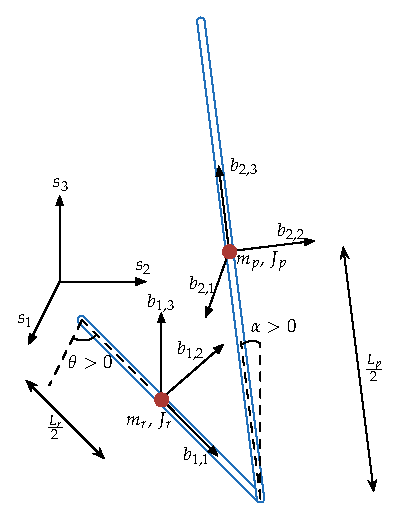
\includegraphics[width=\textwidth]{eps/lab_2/rotary_pendulum_edit.eps}
        \caption{}
    \end{subfigure}
    \caption{(a) Physical rotary pendulum system~\cite{Q-Flex-Beam}; (b) model of the physical system with two rigid bodies connected together, where rigid body 1 (rotary shaft) rotates in the horizontal plane and rigid body 2 (pendulum rod) rotates in the vertical plane. The reference coordinate axes are shown by $\{s_1,s_2,s_3\}$, and the body coordinate axes for rigid bodies 1 and 2 are shown by $\{b_{1,1},b_{1,2}, b_{1,3}\}$ and $\{b_{2,1},b_{2,2},b_{2,3}\}$, respectively. The centres of mass for bodies 1 and 2 are shown in red; the horizontal rotation angle, $\theta$, the vertical rotation angle, $\alpha$, are shown. Important distances are labelled.}
    \label{fig:lab2_rotary_pendulum}
\end{figure}

We will consider two cases: one when the pendulum is in its \textbf{downwards} position (i.e.\ \( \alpha=\pi \)), and one in its \textbf{inverted} position (i.e.\ \( \alpha=0 \)).

\subsection{Setting Up the Rotary Pendulum}
The only thing you should have to do with the rotary pendulum is to turn on the power amplifier. The power switch is located at the back of the amplifier (good luck finding it). Make sure to turn off the power amplifier before you leave the lab.See Appendix~\ref{chap:hardware} for more info on the configuration of the rotary pendulum.

\subsection{Feedback Gain and Pole Placement}\label{subsection:feedback}
Recall that for $A \in \mathcal{M}^{n \times n}(\mathbb{R})$ and for $B \in \mathbb{R}^n$, if the pair $(A,B)$ is controllable, then there exists a transformation $T \in \mathcal{M}^{n \times n}(\mathbb{R})$ where $\text{det}(T) \not = 0$ and
\begin{equation}\label{eq:A_tilde}
    \tilde{A} = TAT^{-1} =
    \left[\begin{array}{c c c c c}
            0      & 1      & 0    & \dots  & 0        \\
            0      & 0      & 1    &        & 0        \\
            \vdots & \vdots &      & \ddots & \vdots   \\
            0      & 0      & 0    & 0      & 1        \\
            -a_0   & -a_1   & -a_2 & \dots  & -a_{n-1}
        \end{array}\right]
\end{equation}
where $\chi_{A} = \chi_{\tilde{A}} = s^n + a_{n-1} s^{n-1} + \dots + a_1 + a_0$ (i.e., $\tilde{A}$ is uniquely determined by the coefficients of the characteristic polynomial of $A$), and
\[
    \tilde{B} = TB =
    \left[\begin{array}{c}
            0      \\
            0      \\
            \vdots \\
            1
        \end{array}\right],
\]
which is called the canonical controllable form (recall that $(A,B)$ is controllable if and only if $(\tilde{A},\tilde{B})$ is controllable since system controllability is invariant under similarity transformations). To find an appropriate feedback gain $K$ for your system~\eqref{equation:lab3_feedback} that will place the system's poles in $\mathbb{C}^-$, you will first design a feedback gain $\tilde{K}$ for the transformed system and then transform $\tilde{K}$ into $K$. To do that, design $\tilde{K} = [k_0, \; k_1, \; \dots, \; k_{n-1}]$ so that you obtain the desired poles:
\[
    \tilde{A}-\tilde{B}\tilde{K} =
    \left[\begin{array}{c c c c  c}
            0          & 1          & 0          & \dots  & 0                  \\
            0          & 0          & 1          &        & 0                  \\
            \vdots     & \vdots     &            & \ddots & \vdots             \\
            0          & 0          & 0          & 0      & 1                  \\
            -(a_0+k_0) & -(a_1+k_1) & -(a_2+k_2) & \dots  & -(a_{n-1}+k_{n-1})
        \end{array}\right]
\]
which yields $\chi_{(\tilde{A}+\tilde{B}\tilde{K})} = s^n + (a_{n-1}+k_{n-1})s^{n-1} + \dots + (a_1 + k_1) + (a_0 + k_0)$. In class, you found an explicit formula for computing the transformation $T$:
\[
    T=\mathcal{C}_{(\tilde{A},\tilde{B})} \mathcal{C}_{(A,B)}^{-1}.
\]

\subsection{Luenberger Observers}
Let us denote the state estimate by $\hat{\mathbf{x}}(t)$. David G. Luenberger proposed the following linear state observer~\cite{david1971introduction}:
\begin{equation}\label{lab3_equ:luenberger}
    \mathbf{\dot{\tilde{x}}}(t)=A\hat{\mathbf{x}}(t)+Bu(t)+L(\mathbf{y}(t)-C\hat{\mathbf{x}}(t)),
\end{equation}
where $L$ is the observer gain. Note that the input and measured output data are both used in~\eqref{lab3_equ:luenberger}. The observer in~\eqref{lab3_equ:luenberger} is composed of two parts: the first part, $A\hat{\mathbf{x}}(t)+Bu(t)$, is the rate of change of $\hat{\mathbf{x}}(t)$ as computed by the physical system's state-space model; the second part, $L(\mathbf{y}(t)-C\hat{\mathbf{x}}(t))$, is the difference between the observed output and the estimated output, scaled by the observer gain. Notice that without the second term, ~\eqref{lab3_equ:luenberger} becomes familiar:
\begin{equation}\label{lab3_equ:luenberger_simple}
    \mathbf{\dot{\hat{x}}}(t)=A\hat{\mathbf{x}}(t)+Bu(t).
\end{equation}
Let us denote the estimation error by $\tilde{\mathbf{x}}(t)$ and define it by $\tilde{\mathbf{x}}(t) = \mathbf{x}(t)-\hat{\mathbf{x}}(t)$. If one were to study the estimation error of the simplified observer~\eqref{lab3_equ:luenberger_simple}, then they would conclude that $\tilde{\mathbf{x}}(t)$ would go to zero when $\text{spec}(A) \subset \mathbb{C}^-$, as the error dynamic for~\eqref{lab3_equ:luenberger_simple} is
\begin{align*}
    \mathbf{\dot{\tilde{x}}}(t) & = A \left(\mathbf{x}(t)-\hat{\mathbf{x}}(t)\right)+Bu(t) - Bu(t) \\
                                & = A\tilde{\mathbf{x}}(t).
\end{align*}
That is, when matrix $A$ has all of its eigenvalues in the left half-plane, then the state estimate would converge to the actual state. But this convergence depends on the physical system's dynamics (thus the convergence rate can be quite slow, depending on the system) and the spectral constraints on $A$ are very restrictive. In contrast, the error dynamic for the Luenberger observer in~\eqref{lab3_equ:luenberger} is
\begin{equation}\label{lab3_equ:luenberger_error}
    \mathbf{\dot{\tilde{x}}}(t) = (A-LC) \tilde{\mathbf{x}}(t).
\end{equation}
Thus one can design an observer gain $L$ such that $\text{spec}(A-LC) \subset \mathbb{C}^-$ (i.e., an \emph{asymptotically stable observer}) and one can tune $L$ such that $\hat{\mathbf{x}}(t)$ converges to $\mathbf{x}(t)$ fast enough for the desired application. An important question to ask is, ``when does such an observer exist"? In class, you proved that one can build an observer with these properties when $(C,A)$ is \emph{detectable}.

\subsection{Control Technique}
In this lab, you will be designing a feedback controller that stabilizes the system about the inverted pendulum orientation. That is, to balance the pendulum in the inverted orientation, you must design a feedback gain that renders the closed-loop system \emph{internally asymptotically stable}. Note that the state space matrices are based on linearization techniques, so they are only a good approximation on a limited domain. So when designing the balance controller, you will need to lift up the pendulum from the downwards orientation to the inverted orientation while holding the servo base, and then have the controller engage in a small domain centered at the unstable equilibrium. Thus, the controller will be of the form
\[ u(t) =
    \begin{cases}
        K(\mathbf{x_d} - \mathbf{x}(t)) \quad |\alpha| < \epsilon; \\
        \quad \quad 0 \quad \quad \quad \quad \text{otherwise},
    \end{cases}
\]
where $\epsilon$ is the angle designating when the controller will engage and $x_d$ is the desired reference state. To balance the pendulum in the inverted orientation, one should choose a desired reference state of
\[
    \mathbf{x_d} =
    \left[\begin{array}{c}
            \theta_d \\
            0        \\
            0        \\
            0
        \end{array}\right]
\]
where $\theta_d$ is a desired rotor base angle (one may wish that the rotor base track a desired trajectory, thus $\theta_d=\theta_d(t))$. To design an appropriate control gain that will balance the inverted pendulum, consider our closed-loop system when the controller is engaged:
\begin{equation}
    \begin{cases}
        \mathbf{\dot{x}}(t) = \left(A-KB\right)\mathbf{x}(t) + B\mathbf{x_d}; \\
        \mathbf{y}(t) = C\mathbf{x}(t).
    \end{cases}
    \label{equation:lab3_feedback}
\end{equation}

You can use these results to design the appropriate feedback gain $K$ to balance the inverted pendulum.

\subsection{Matrices}\label{section:lab3_prelab}
The following sections will provide relevant matrices/equations for the lab. If you're interested in the derivation of these matrices, you can find more info in Appendix~\ref{chap:EOMs}. Make sure you use the correct matrices based on the position of the pendulum.

\subsubsection*{Downwards Position (\( \theta_0=0, \alpha_0=\pi \))}
\[
    A =
    \left[\begin{array}{c c c c}
            0 & 0       & 1      & 0       \\
            0 & 0       & 0      & 1       \\
            0 & 81.38   & -93.49 & 0.0038  \\
            0 & -122.03 & 89.97  & -0.0058 \\
        \end{array}\right]
\]

\[
    B =
    \left[\begin{array}{c}
            0     \\
            0     \\
            83.64 \\
            -80.48
        \end{array}\right].
\]

\subsubsection*{Inverted Position (\( \theta_0=0, \alpha_0=0 \))}
\[
    A =
    \left[\begin{array}{c c c c}
            0 & 0      & 1      & 0     \\
            0 & 0      & 0      & 1     \\
            0 & 81.38  & -46.05 & -0.93 \\
            0 & 122.03 & -44.31 & -1.39
        \end{array}\right],
\]
\[
    B =
    \left[\begin{array}{c}
            0     \\
            0     \\
            83.64 \\
            80.48
        \end{array}\right],
\]

For both positions, given that the physical system’s sensors are limited to reading the rotor angle and the deflection angle, our state space matrices \(C\) and \(D\) are

\[
    C =
    \left[\begin{array}{c c c c}
            1 & 0 & 0 & 0 \\
            0 & 1 & 0 & 0
        \end{array}\right]
\]
and
\[
    D =
    \left[\begin{array}{c}
            0 \\
            0
        \end{array}\right].
\]

\section{Procedure}
\begin{enumerate}
    \item \textbf{Pole Placement \& Full State Feedback}\label{section:lab3_feedback}
          \begin{enumerate}
              \item The open loop poles can be found by computing the roots of the system's characteristic equation, i.e., finding the roots of \( \text{det}(sI-A)=0 \). In MATLAB, this is easily done by using the command \( eig(A) \). Compute the open-loop poles for each position (the downwards and the inverted).
              \item Is each open-loop system stable? Does this make physical sense?
                    %The open loop poles can be found by computing the roots of the system's characteristic equation, i.e., finding the roots of $\text{det}(sI-A)=0$. In MATLAB, this is easily done by using the command $eig(A)$. The open-loop poles are
                    %\[
                    %\{-48.63, \; 7.05, \; -5.86, \; 0\}.
                    %\]
                    %It can be concluded that the system is internally unstable about the chosen equilibrium as $\text{spec}(A) \cap \mathbb{C}^+ \not = \emptyset $. This makes physical sense as the inverted pendulum is not in a stable orientation and any perturbation about this equilibrium point will drive the pendulum away from the inverted orientation.

                    %Yes, the linearized system about the pendulum resting downwards is internally stable, as $\text{spec}(A) \cap \mathbb{C}^+ = \emptyset $:
                    %\[
                    %\{-45.24, \; -1.11 + 6.57i, \; -1.11 - 6.57i, \; 0\},
                    %\]
                    %and since for each eigenvalue $ \lambda \in \text{spec}(A)$, its geometric multiplicity equals its algebraic multiplicity (since $A \in \mathcal{M}^{4\times4}$ and there are four distinct eigenvalues of A, thus there is one eigenvector for each corresponding eigenvalue). This makes physical sense because when the pendulum is perturbed from this equilibrium point, it returns to it.

                    \textbf{The following questions all concern the \emph{inverted} position.}

              \item Can we hope to use full state feedback to steer the linearized rotary pendulum system? \textbf{Hint:} This has to do with the controllability of the system.
                    %\drew{Answer: To verify this, one must compute the controllability matrix of the system:
                    %\[
                    %\mathcal{C}_{(A,B)} = 
                    %\left[\begin{array}{c c c c}
                    %0 & 83.64 & -3926.74 & 190939.11\\
                    %0 & 80.48 & -3818.93 & 189168.17\\
                    %83.64 & -3926.74 & 190939.11 & -9279982.88\\
                    %80.48 & -3818.93 & 189168.17 & -9191635.19
                    %\end{array}\right]
                    %\]
                    %The system's controllability matrix has full rank, and hence the system is controllable. Thus, we can hope to use full state feedback and pole placement techniques to control the system.}
              \item Find the coefficients of the characteristic polynomial for your open-loop state-space model by multiplying the eigenvalues together, as shown in the following:
                    \[
                        \chi_{A} = (s-\lambda_1)(s-\lambda_2)(s-\lambda_3)(s-\lambda_4) = s^4 + a_3 s^3 + a_2 s^2 + a_1 s^1 + a_0.
                    \]
                    What is $\tilde{A}$? (see~\eqref{eq:A_tilde})
                    %\drew{Answer: You should get
                    %\[
                    %\tilde{A} = 
                    %\left[\begin{array}{c c c c}
                    %0 & 1 & 0 & 0\\
                    %0 & 0 & 1 & 0\\
                    %0 & 0 & 0 & 1\\
                    %0 & 2013.52 & 98.98 & -47.44
                    %\end{array}\right].
                    %\]
                    %}
              \item Find a $\tilde{K}$ such that the poles of the closed-loop system are $\{-2.8 + 2.86i, \; -2.8 - 2.86i, \; -30, \; -40\}$.
                    \textbf{Hint:} You can use the \emph{sym2poly(p)} MATLAB command to find the coefficients of the characteristic polynomial generated by the desired poles. The coefficients you get from this will be \( a_i + k_i \), and you have to solve for \( k_i \).
                    %\drew{Answer: You should get
                    %\[
                    %\tilde{K} = [19223.52 \quad 9854.89 \quad 1707.00 \quad 28.15].
                    %\]
                    %You get this by the following MATLAB commands:
                    %\[\begin{aligned}
                    %a=poly(A);\\
                    %syms \hspace{2mm}s;\\
                    %b=sym2poly((s-(-2.8 + 2.86i))*(s-(-2.8 - 2.86i))*(s-(-30))*(s-(-40)));\\
                    %K\_tilde = [b(5)-a(5) b(4)-a(4) b(3)-a(3) b(2)-a(2)];
                    %\end{aligned}\]
                    %}
              \item Calculate the transformation $T=\mathcal{C}_{(\tilde{A},\tilde{B})} \mathcal{C}_{(A,B)}^{-1}$. A quick way to find $\mathcal{C}_{(A,B)}$ is to use the \emph{ctrb(A,B)} MATLAB command. What is the ensuing feedback gain, $K$?
                    \textbf{Hint:} $A-BK= T^{-1}(TAT^{-1} - TBKT^{-1})T \implies A-BK = T^{-1}(\tilde{A}-\tilde{B}\tilde{K})T$, thus $K=\tilde{K}T$.\\
                    %\drew{Answer: You should get
                    %\[
                    %K = [-5.25 \quad 28.10 \quad -2.75 \quad 3.21].
                    %\]
                    %}

                    You will now use this feedback gain to experimentally balance the physical rotary pendulum system. Open \textbf{balancing\_model.mdl} and make sure that your state-space matrices $A$, $B$, $C$ and $D$ as well as your feedback gain $K$ is loaded in the MATLAB workspace. The Simulink model is shown in Figure~\ref{lab3_simulink_balance}. The feedback controller is activated by the Control Switch block when the pendulum angle is within an $\epsilon$-range of $\alpha = 0$ (recall that $\alpha=0$ corresponds to the pendulum being completely inverted). While the system is balancing the inverted pendulum, you will input to the system a square wave of amplitude 10, so that the servo motor (and hence $\theta$) tracks the square wave. So you must first get the pendulum to balance by keeping the Amplitude block at 0, \textbf{then} changing the Amplitude block to 10. Note that you will have to hold the servo motor when initially lifting the pendulum to the inverted orientation, and then let it go once the pendulum is completely inverted. It may take a few tries to get the pendulum to balance.

                    The curious reader may concerned with the workings of the Find State X subsystem block found in the Simulink model shown in Figure~\ref{lab3_simulink_balance}. This subsystem block uses a numerical differentiator technique to find the derivative estimations of the measured signals, $\theta$ and $\alpha$. This technique is based on using a high-gain observer~\cite{dabroom1999discrete} to estimate the derivatives of the signals. While the angular velocity of the rotor base and the pendulum are not measured and outputted from the physical system (neither are they outputted from the state-space model), one can usually estimate these variables by using such methods.
                    \begin{figure}[htb!]
                        \centering
                        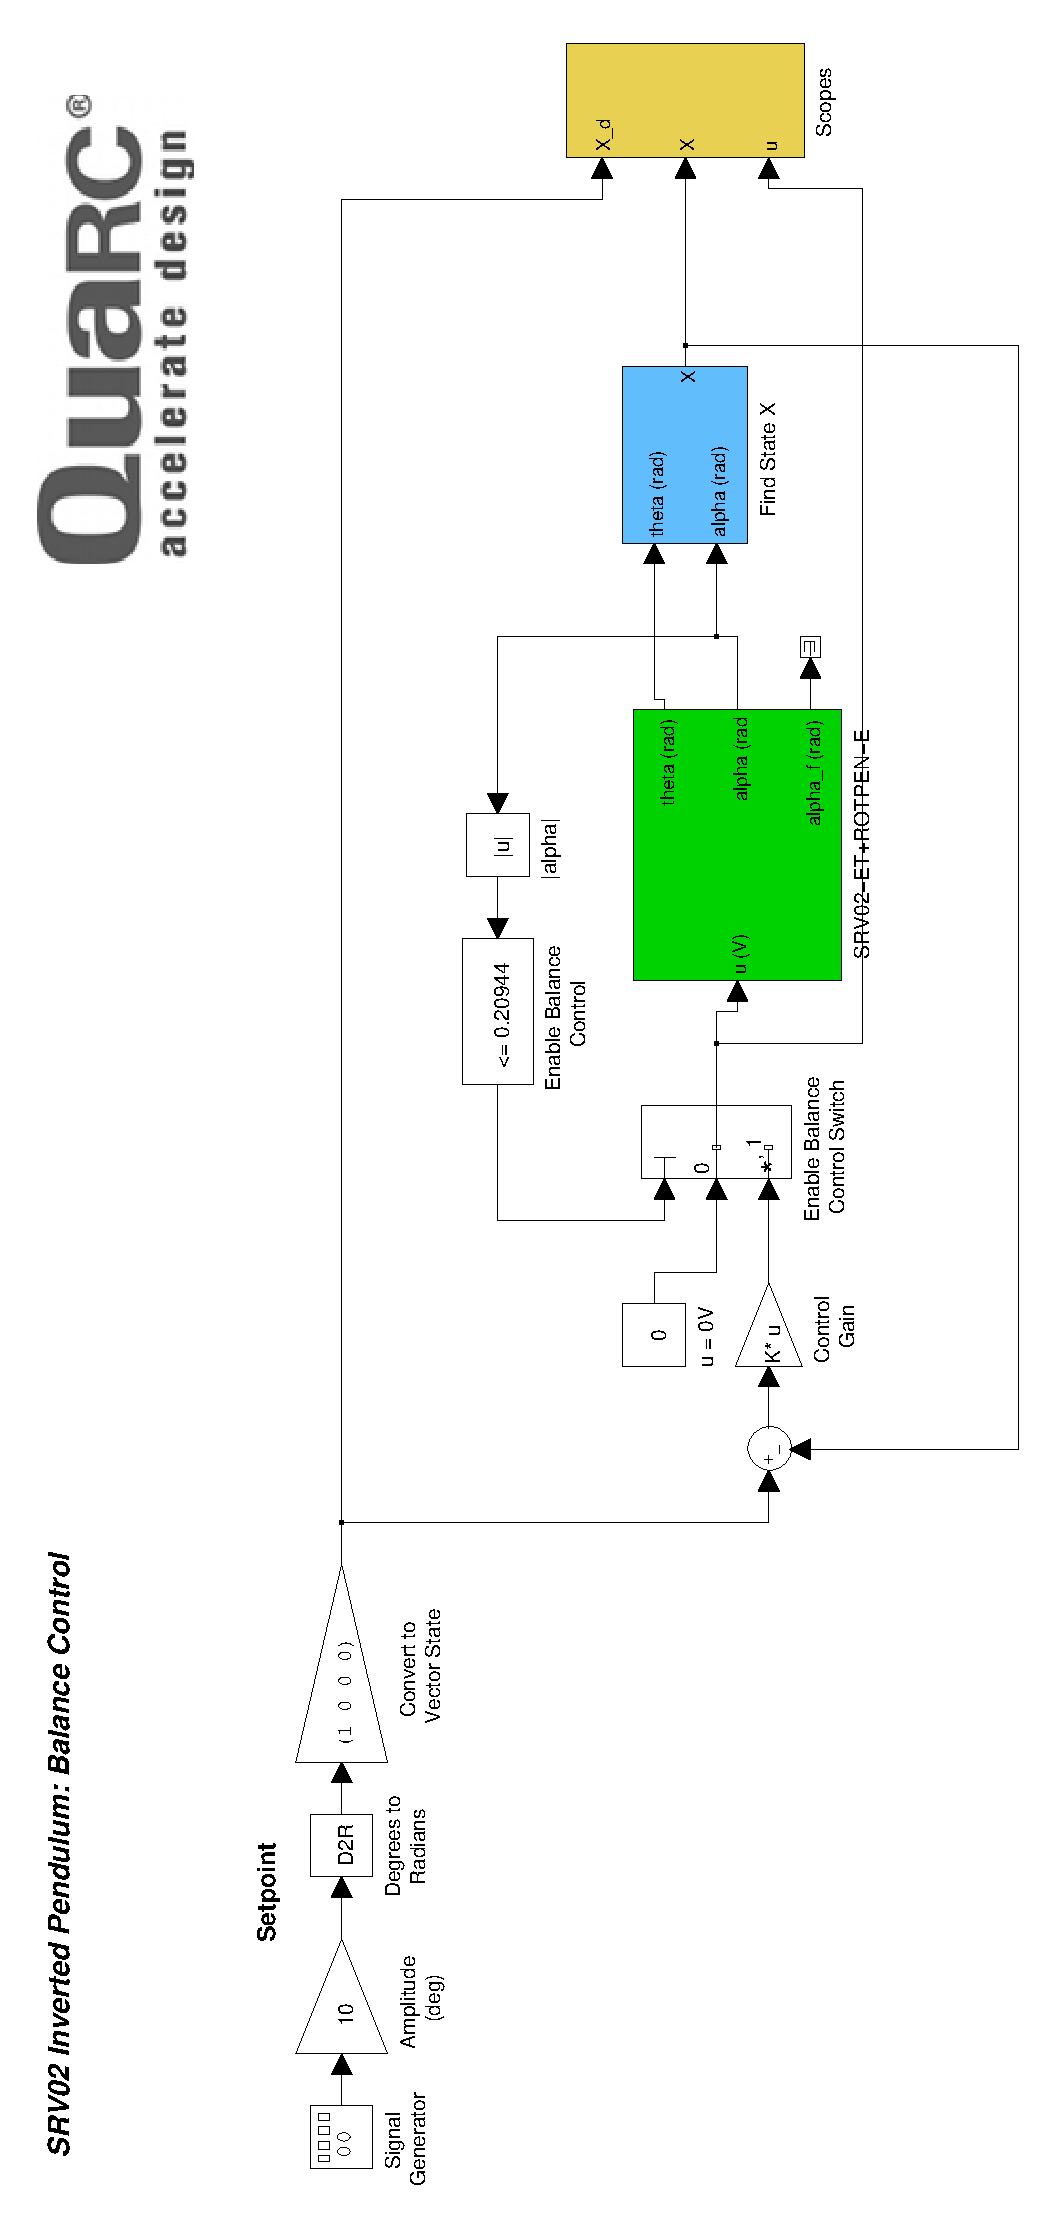
\includegraphics[width=0.5\linewidth,angle=-90]{eps/lab_3/balance_controller.eps}
                        \caption{A Simulink model which interacts with the physical rotary pendulum system and uses state feedback in a small domain about the unstable equilibrium (i.e., inverted pendulum orientation) to balance the inverted pendulum.~\cite{Q-Flex-Beam}}
                        \label{lab3_simulink_balance}
                    \end{figure}
                    \newpage
              \item Record the results of the balancing experiment and plot your data. On one plot, compare the square wave input for the rotor base and the measured rotor base angle, $\theta$. On another plot, include the pendulum angle data, $\alpha$. Does your feedback controller manage to balance the inverted pendulum while tracking the square wave trajectory? What happens if you keep increasing the square wave amplitude, and why does this happen? What happens when you change the poles of the closed-loop system to be more negative in the left half-plane of $\mathbb{C}$ (i.e., designing the feedback gain, $K$, such that the closed-loop poles are much more negative)? For balancing the inverted pendulum, discuss the \emph{trade-offs between designing} the control system such that the poles of the closed-loop system are close to the origin or far in the left half-plane.
                    %\drew{Answer: Yes, it should be able to balance the inverted pendulum while tracking the square wave with amplitude of 10. If the amplitude is increased, then the pendulum angle may exceed the domain of validity of the linearization, and the feedback controller may not be able to balance the inverted pendulum.  Instructors should note that students' answers will vary, as the tension in the slip-gear will change the input required to balance the pendulum. When changing the poles of the closed-loop system by changing $F$, you change the rate of stabilization and the overshoot/undershoot of the stabilization. If one were to place these poles far in the left half-plane, then stabilization would be very immediate, but this immediate response comes at the cost of a large overshoot. In the case of the inverted pendulum, where the linearized system is only valid in a small neighbourhood about the inverted orientation, a large overshoot may be detrimental. Conversely, a very slow stabilization may allow the pendulum to fall outside the linearization's domain of validity, which also causes negative effects. Hence one must design and tune the feedback gain, $K$, for this application such that balancing stabilization is achieved quickly enough without a large overshoot. Here are the plots:
                    %\begin{figure}[htb!]
                    %\centering
                    %	\subfigure{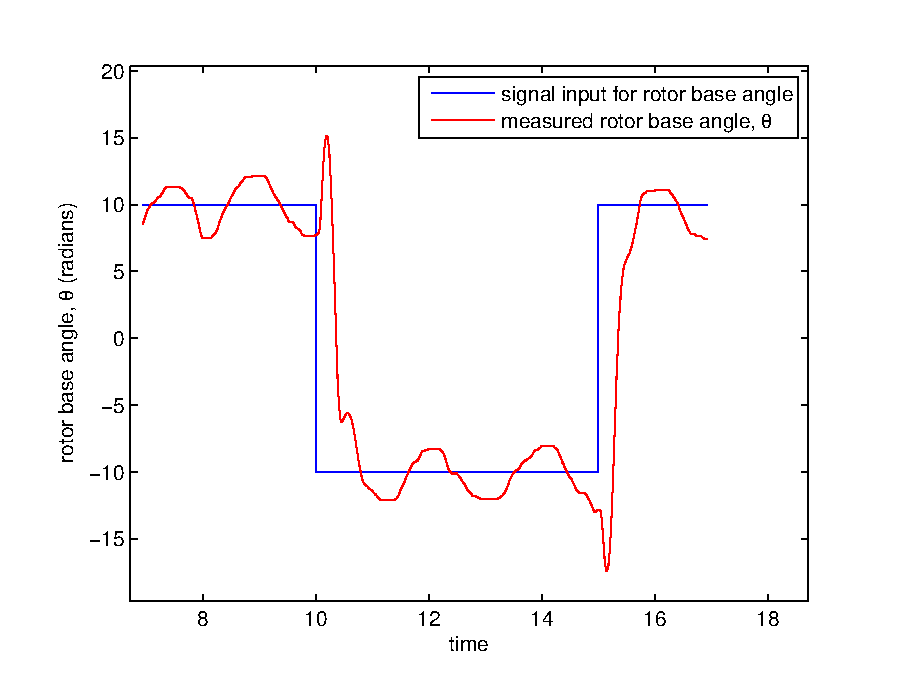
\includegraphics[width=0.4\linewidth]{eps/lab_3/full_feedback_balance_thetas.eps}} \quad
                    %	\subfigure{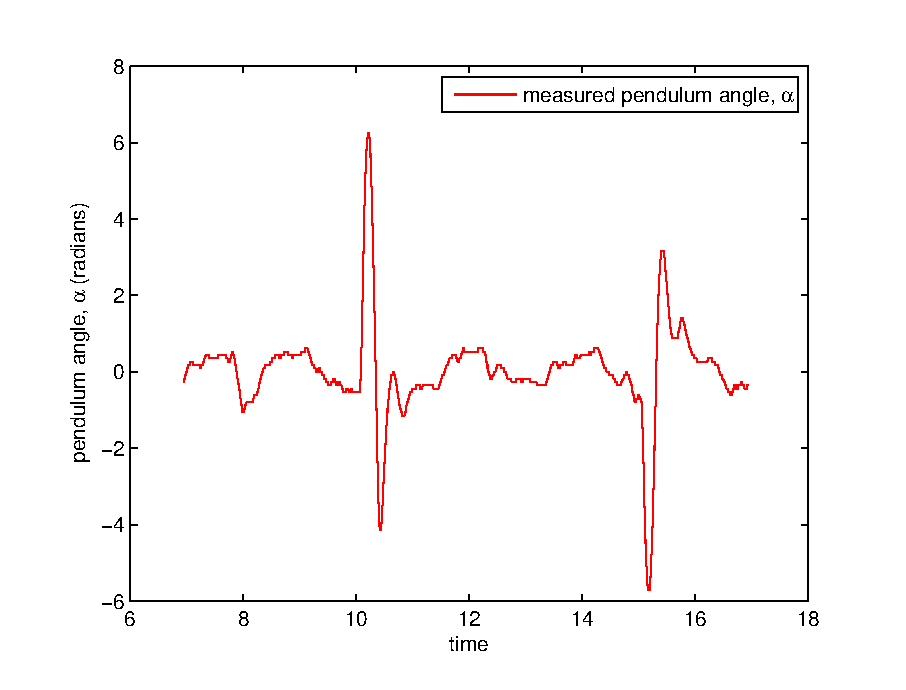
\includegraphics[width=0.4\linewidth]{eps/lab_3/full_feedback_balance_alpha.eps}}
                    %	\caption{(a) A plot of the desired and measured rotor base angle trajectories for the closed-loop feedback controller system while balancing the pendulum in the inverted orientation and while the rotor base tracks a square wave trajectory with amplitude 10, and; (b) a plot of the measured pendulum angle while the physical system tracks this square wave trajectory.}
                    %	\label{fig:lab3_state_feedback_response}
                    %\end{figure}
                    %}
          \end{enumerate}
    \item \textbf{Linear Observer}\label{section:lab3_observer}
          \begin{enumerate}
              \item
                    Recall our linear time-invariant system dynamics
                    \[\mathbf{\dot{x}}(t)=A\mathbf{x}(t)+Bu(t) \quad \quad \quad \mathbf{y}(t)=C\mathbf{x}(t)\]
                    and consider the case where the encoder that reads the pendulum angle is damaged, i.e.,
                    \[C = \left[\begin{array}{c c c c}
                                1 & 0 & 0 & 0 \\
                                0 & 0 & 0 & 0
                            \end{array}\right]\]
                    In this case, you do not have access to one of the system's internal states, $\alpha$. However, you may be able to determine the unknown state by using the system's input and output data. To do this, you will construct a linear dynamical system that produces an estimate of the physical system's state, also known as a \emph{linear state observer}.

                    \textbf{The following questions all concern the \emph{downwards} position.}
              \item When the reader for the pendulum angle is damaged (i.e.\ the matrix \(C\) is as above), can you hope to observe the unknown state $\alpha$ by designing and building an appropriate state observer? What does system detectability mean, and is the system detectable? \textbf{Hint:} Compute the observability matrix of the system.

                    %\drew{Answer: Yes; since the system is observable when 
                    %\[C = \left[\begin{array}{c c c c}
                    %1 & 0 & 0 & 0\\
                    %0 & 0 & 0 & 0
                    %\end{array}\right],\]
                    %it is also detectable, as detectability is a weaker notion of observability. System detectability implies that all of the system's unobservable states are asymptotically stable, but there are no unobservable states for this system.
                    %}
                    One way to \emph{design an observer is by eigenvalue assignment}: the Luenberger observer error, $\tilde{\mathbf{x}}(t)$, governed by the differential equation~\eqref{lab3_equ:luenberger_error}, has a characteristic polynomial chosen by the designer. That is, the observer designer chooses $L$ such that the eigenvalues of $(A-LC)$ are at desired locations $p_1, p_2, \dots, p_n$. This design method has some benefits over other methods, mainly:
                    \begin{itemize}
                        \item theoretically, the observer error can decrease faster if the eigenvalues of $(A-LC)$ are more negative (however, there is a trade-off which you will explore), and;
                        \item if the observed states are being used for state feedback, then the least negative eigenvalue of $(A-LC)$ should be more negative than the eigenvalues of the state feedback system $A-BK$. Loosely speaking, this dictates that the observer dynamics will converge to the unobserved states \emph{faster} than the system dynamics will change these states.
                    \end{itemize}
                    One may notice a similarity between finding a feedback gain $K$ such that $A-BK$ has eigenvalues in $\mathbb{C}^-$ and finding an observer gain $L$ such that $A-LC$ also has eigenvalues in $\mathbb{C}^-$. Recall that the eigenvalues of a matrix and its transpose are the same. The problem of observer design is in fact the \emph{dual} of the state feedback problem, with the following equivalences~\cite{astrom2010feedback}:
                    \begin{align*}
                        (A-LC)^T                      & = A^T - C^T L^T                                  \\
                                                      & \leftrightarrow A - BK                           \\
                        \\
                        A \leftrightarrow A^T \quad B & \leftrightarrow C^T \quad K \leftrightarrow L^T.
                    \end{align*}

                    In Section~\ref{section:lab3_feedback}, you solved for $K$ by using the canonical controllable form and a similarity transformation. In MATLAB, there's a shortcut to solving for $K$ which uses the \emph{place} command. To solve for the feedback gain with desired poles at $\{-2.8 + 2.86i, \; -2.8 - 2.86i, \; -30, \; -40\}$, you can do the following in MATLAB:
                    \[
                        p = [-2.8 + 2.86i \quad -2.8 - 2.86i \quad -30 \quad -40];
                    \]
                    \[
                        K = place(A,B,p);
                    \]

              \item In MATLAB, how could you use the \emph{place} command to design observer gain $L$ such that $A-LC$ has its poles at $p =\{p_1, \; p_2, \; p_3, \; p_4\}$? What is the resulting gain \(L\)? \textbf{Hint:} Use the above duality equations.
                    %\drew{Answer: Using the duality of the observer and feedback design problems, and the equivalences stated above, you could use the MATLAB command
                    %\[
                    %L = place(A',C',p)';
                    %\]
                    %to complete the task.}
          \end{enumerate}

    \item \textbf{Designing \& Validating an Observer}\label{sub section:lab3_observer_design}

          You will now design an observer for the linearized rotary pendulum system, linearized about the \emph{stable equilibrium} (downwards position). You will use the $C$ matrix so that only the rotor base angle, $\theta$, is outputted, as you are studying the case where the encoder reading the pendulum angle is damaged (i.e.\ the \(C\) matrix in the previous section). Figure~\ref{figure:lab3_luenberger_block} shows a Simulink block diagram for a Luenberger observer; you will integrate this observer subsystem into a Simulink model to compare the actual and estimated states.
          \begin{figure}[htb!]
              \centering
              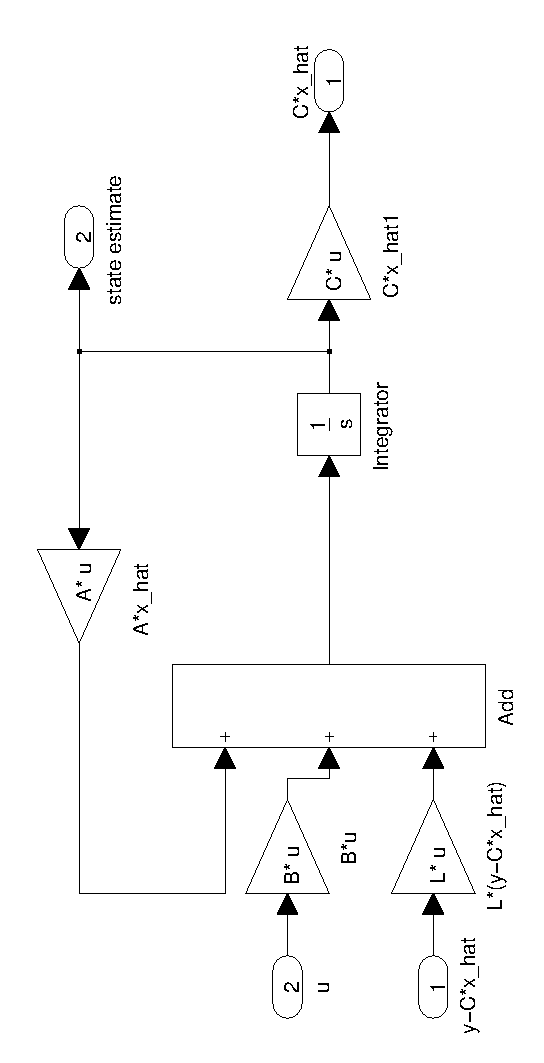
\includegraphics[width=0.4\linewidth,angle=-90]{eps/lab_3/luenberger_subsystem}
              \caption{A Simulink block diagram of a Luenberger observer. This is a subsystem block that can be incorporated into a Simulink model, along with a state-space subsystem block, to compare the estimated and the actual states.}
              \label{figure:lab3_luenberger_block}
          \end{figure}

          Open the Simulink model \textbf{luenberger\_openloop\_model.mdl}. Note that the regular State-Space block is not used to model the linearized rotary pendulum system; in place, we've created a subsystem block that does this, and it is shown in Figure~\ref{figure:lab3_statespace_block} along with the Luenberger observer subsystem block.
          %The state-space subsystem that we've created allows you to access all of the system's states at a given time and output them into the MATLAB workspace, whereas the State-Space block only outputs $y=Cx$. Thus, you must use this subsystem block for the state-space dynamics so that you can compare the actual states and the state estimates produced by your observer.
          \begin{figure}[htb!]
              \centering
              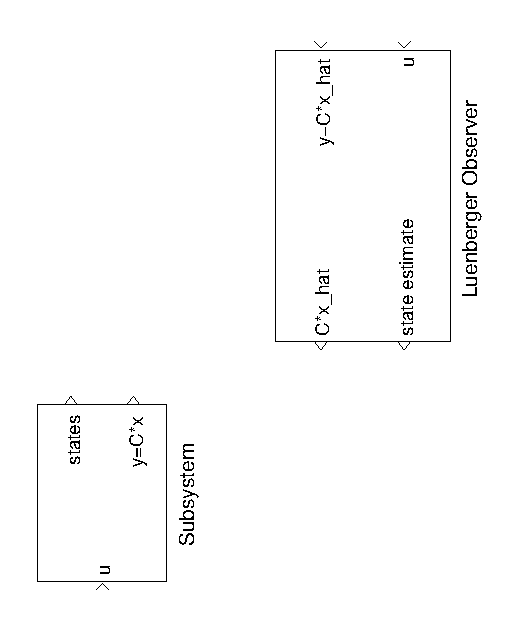
\includegraphics[width=0.4\textwidth,angle=-90]{eps/lab_3/luenberger_openloop_student}
              \caption{A Simulink block diagram of a state-space subsystem \& Luenberger observer subsystem. The state-space subsystem block allows one to output the usual $y=Cx$ output as well as outputting all of the states at each time, making it useful for state estimate validations.}
              \label{figure:lab3_statespace_block}
          \end{figure}

          Connect these two Simulink subsystem blocks so that the observer can estimate the states of the linearized state-space model of the rotary pendulum. Now, add a Signal Generator block, a Sum or Add block, and a DegreesToRadians block to the Simulink model and use a sine signal with amplitude 10 as your input (transforming your input to radians using the DegreesToRadians block). In the state-space subsystem, set the initial conditions (found in the integrator block) of your states to zero (in MATLAB, this is done with the vector $[0;0;0;0]$), and set the initial conditions of your observer subsystem to non-zero values between $[-10,10]$. Make sure to output your states and your state estimates to your workspace using To Workspace blocks.

          \begin{enumerate}
              \item Run various tests using this model while changing the observer's poles in $\mathbb{C}^-$. First, \emph{design and tune your observer} so that the state estimates converges to the actual states very quickly; second, try to achieve state estimates that don't deviate from the actual states too much. \emph{What metrics you would use to evaluate} your observer (and the resulting observer gain design) were it to be used for: state feedback to balance the inverted pendulum, and; monitoring an industrial process where large spikes cause the industrial plant to shut down. \vspace{0.5em}
                    %\drew{Answer: Tuning the observer gain such that the state estimates converge very quickly to the actual states (i.e., the observer poles are far in the left half-plane) comes at the cost of a very large overshoot. Thus, it is important to design the observer gain so that this tradeoff be exploited for a given application. For the inverted pendulum application, since the domain of validity for the linearized system is a small neighbourhood about the inverted orientation, a large overshoot in the pendulum angle state estimation would make the ensuing feedback response overcompensate unnecessarily. Conversely, a slow state estimate convergence can make the ensuing feedback response much to slow to keep the inverted pendulum in the linearized system's domain of validity. This is why this physical stabilization problem is not considered - it is much too finicky to work, and may require techniques other than gain tuning to make it work properly. Some metrics may include overshoot, settling time, energy used in state feedback, etc. For the monitoring application, one would choose to design the observer poles close to the origin since large state estimate overshoots would cost the industrial plant much lost time. The main metric here is overshoot, among other engineering metrics.}

                    Now you will verify that the observer you built for the state-space model works for the physical system. This will help you identify the benefits and drawbacks of different observer tunings for gain $L$. Open the Simulink model \textbf{luenberger\_openloop\_quanser.mdl}. When accessing the rotary pendulum subsystem block, one will notice that the Luenberger observer is nested into this subsystem, as shown in Figure~\ref{figure:lab3_luenberger_openloop_quanser}. This subsystem outputs the measured and the estimated pendulum angle, so that these angles can be compared directly.
                    \begin{figure}[htb!]
                        \centering
                        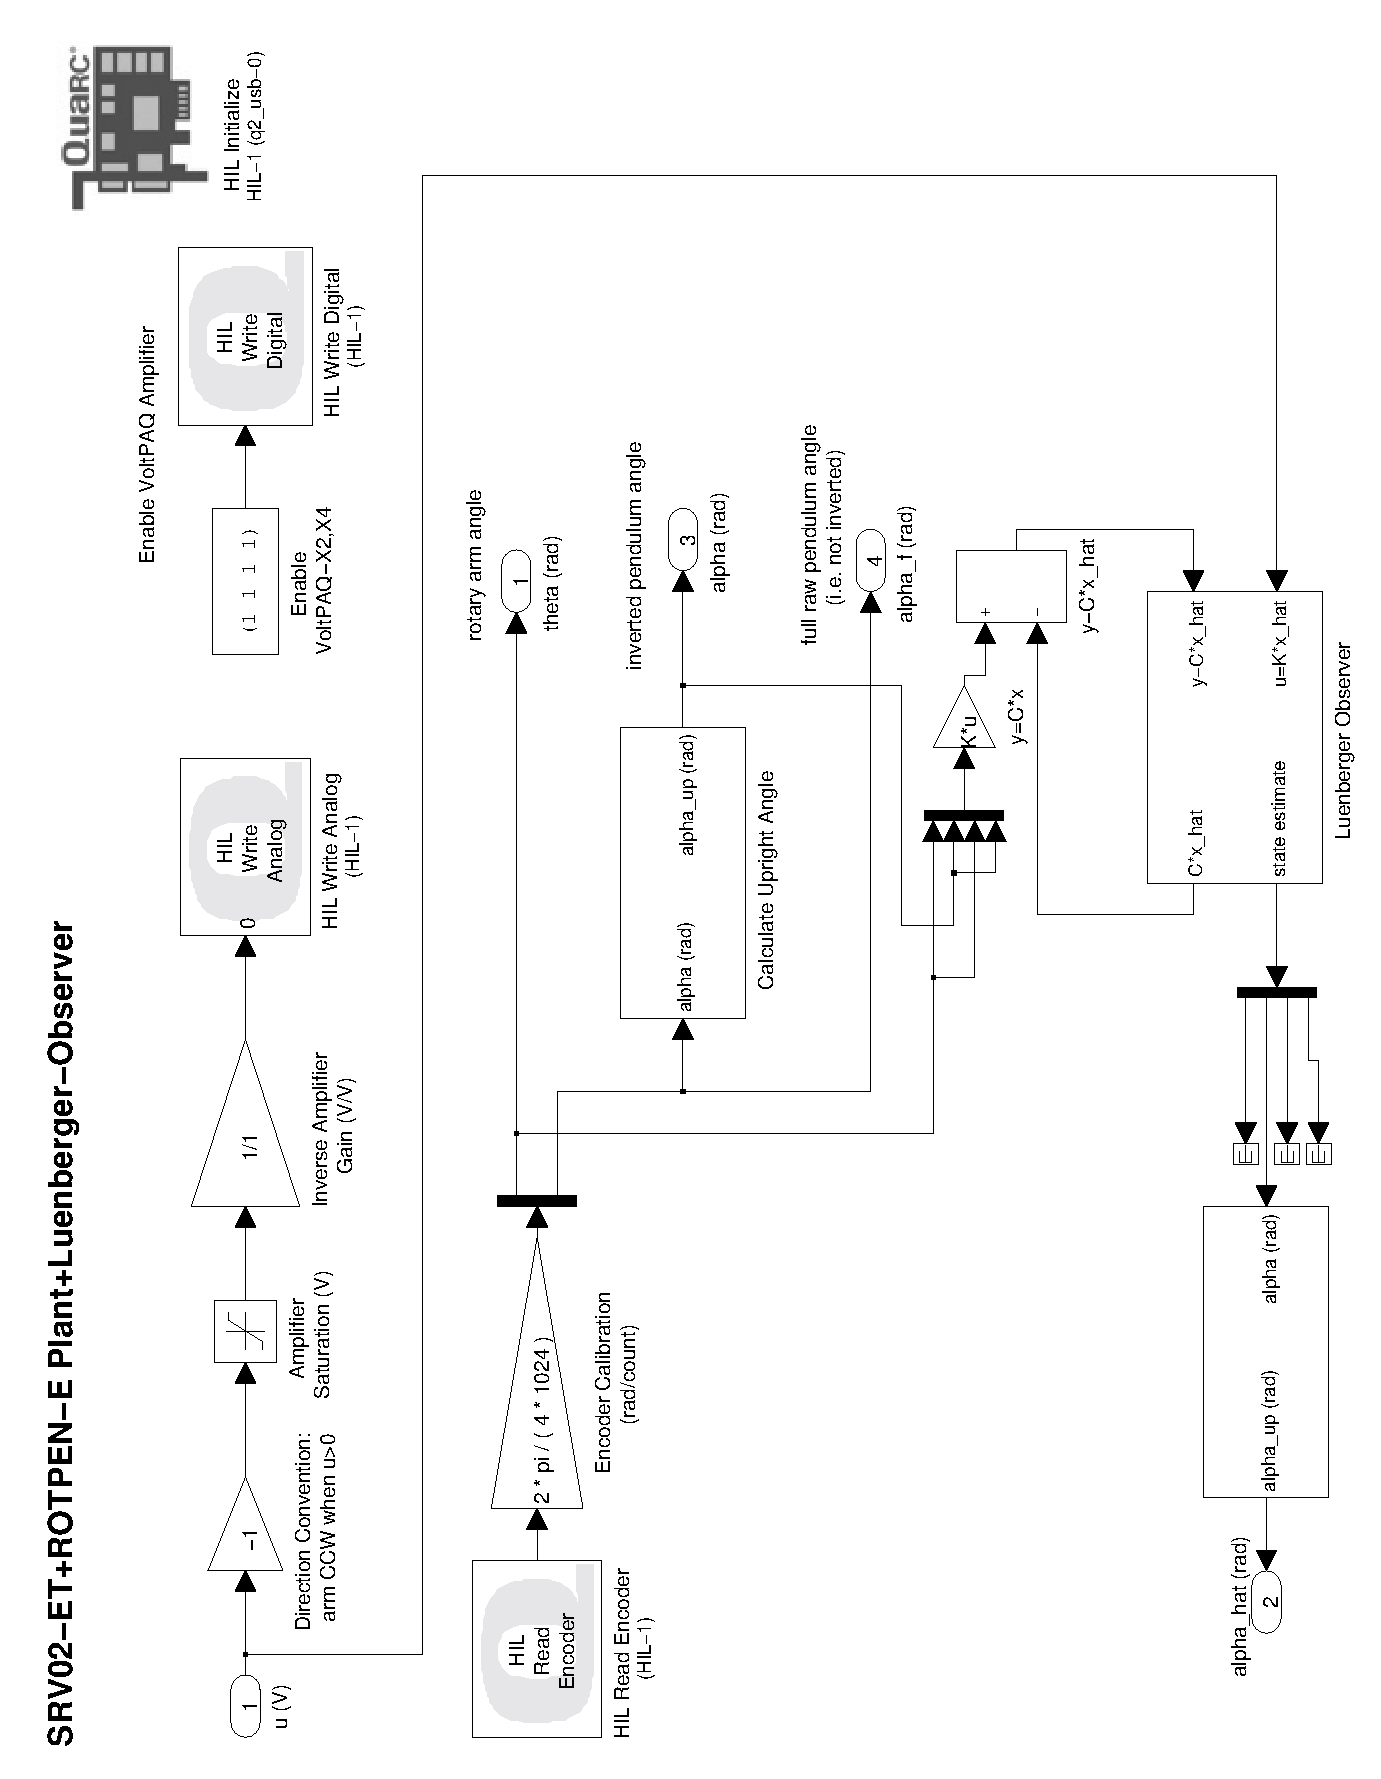
\includegraphics[width=0.6\linewidth,angle=-90]{eps/lab_3/luenberger_openloop_quanser}
                        \caption{A Simulink model of a Luenberger observer estimating \& outputting the pendulum angle, $\hat{\alpha}$, for the physical rotary pendulum system. Note that in the Luenberger observer, measured states $\dot{\theta}$ and $\dot{\alpha}$ are non needed, as they are scaled by $C$.}
                        \label{figure:lab3_luenberger_openloop_quanser}
                    \end{figure}
                    \newpage
              \item Build \& run \textbf{luenberger\_openloop\_quanser.mdl}, with a sine wave input with amplitude of 1 and frequency of 5 $rad/s$. First, use [0,\; 0,\; 0,\; 0] as the initial conditions for the observer. Plot the measured and the estimated pendulum angle, $\alpha$ and $\hat{\alpha}$, with respect to time when your observer has poles $\{-5,\; -6,\; -7,\; -8\}$. Repeat the experiment for observer poles $\{-15,\; -16,\; -17,\; -18\}$, and then for observer poles $\{-45,\; -46,\; -47,\; -48\}$ (creating the same plots for each experiment). Repeat these for the case where the initial conditions of the observer are not identically zero. From these plots, what can you conclude about the relationship between the accuracy of the state estimates produced by your Luenberger observer and \emph{the design and tuning} of the observer gain, $L$? Give two different real-life applications where state observers could be used, and what \emph{metrics} would you develop to evaluate these observers in the setting of their respective applications (specifically look at the relationship between observer behaviour and pole placement via observer gain, $L$).
                    %\drew{Answer: one will note that the observer error after a crest of the sine wave input cannot be completely eliminated for these three observer gains, as some observer error is present in all three plots. The penalty for having very negative observer poles is apparent: while the observer dynamic is very fast, it quickly acts on a control input and then reacts to reduce the estimate output error term ($L(y-C\hat{x}(t)$), and does so frequently. For observer poles at $\{-15,\; -16,\; -17,\; -18\}$, the observer gives a most accurate estimate, but the observer is still a bit too sensitive to control inputs. Due to the constant change in the input signal, the observer estimate error never has time to converge to zero. I will leave the engineering-based responses to be answered by the current TA.
                    %\begin{figure}[htb!]
                    %\centering
                    %\subfigure{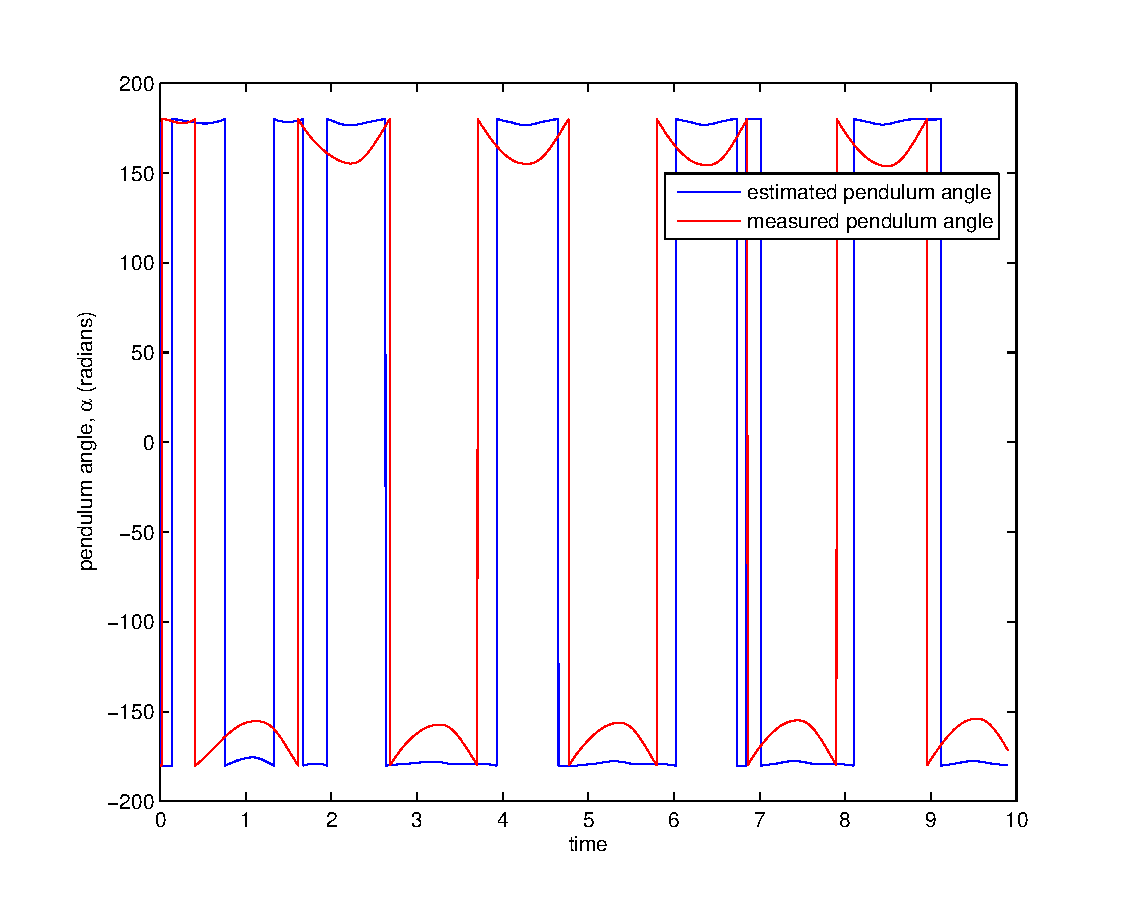
\includegraphics[width=0.4\linewidth]{eps/lab_3/luenberger_openloop_quanser_exp1}}
                    %\subfigure{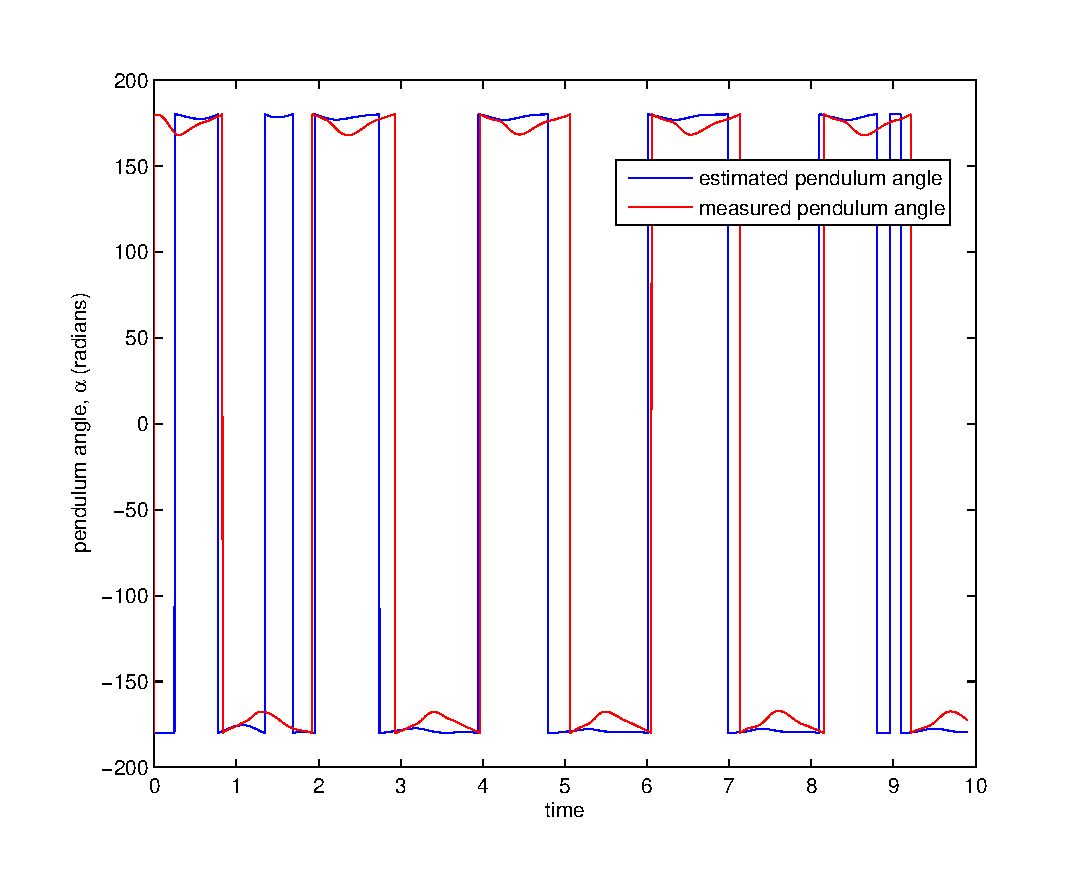
\includegraphics[width=0.4\linewidth]{eps/lab_3/luenberger_openloop_quanser_exp2}}
                    %\subfigure{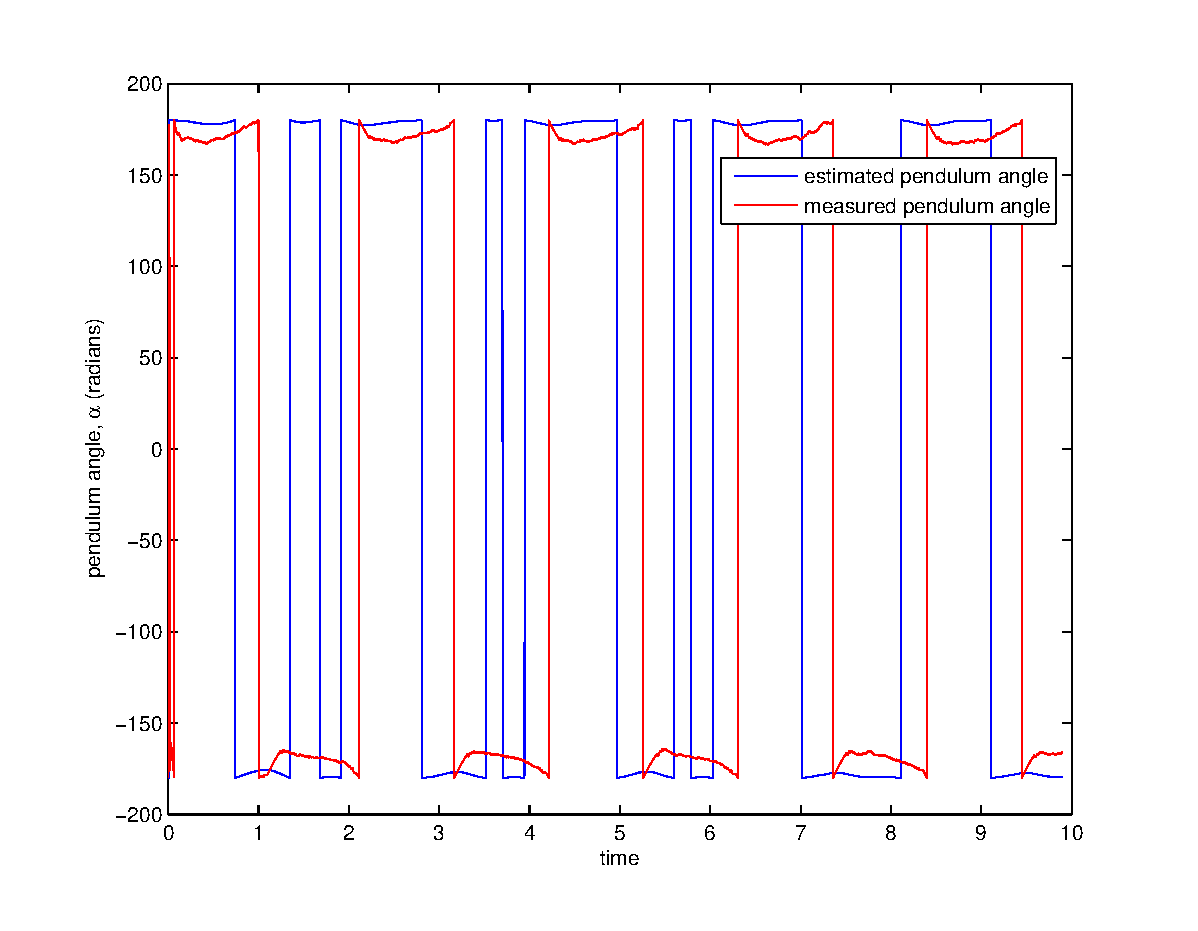
\includegraphics[width=0.4\linewidth]{eps/lab_3/luenberger_openloop_quanser_exp3}}
                    %\caption{Plots comparing the measured and estimated pendulum angle response to a sine wave input of amplitude of 0.5 and frequency of 3 $rad/s$ for observer gains a) $L = \{-5,\; -6,\; -7,\; -8\}$, b) $L = \{-15,\; -16,\; -17,\; -18\}$ and c) $L = \{-45,\; -46,\; -47,\; -48\}$.}
                    %\end{figure}
                    %}
          \end{enumerate}

          %\newpage
          %\subsection{Balance Feedback Control using State Estimate}\label{subsection:lab3_observer_feedback}
          %Now, you'll verify whether you can use your state estimate of $\alpha$, denoted $\hat{\mathbf{\alpha}}$, as well as your measured state, $\theta$, to construct a feedback loop which will make the linearized rotary pendulum system, linearized about the \emph{unstable equilibrium} (i.e., inverted orientation), asymptotically stable.
          %
          %\begin{enumerate}[Questions]
          %\item[Q9:] Is the linearized rotary pendulum system, linearized about $\alpha = 0$ (unstable equilibrium), \emph{detectable}, and why? Is it \emph{stabilizable}, and why? What can be concluded about the viability of using $\hat{\mathbf{\alpha}}$ and $\theta$ as feedback to balance the rotary pendulum in the inverted orientation?\\
          %\drew{Answer: Recall that a system is said to be \emph{detectable} if and only if all of its unstable modes are observable (i.e., if all of its unobservable modes are asymptotically stable). Another way to see this is the following: a system is said to be detectable if $\mathbf{y}(t) \rightarrow 0$ implies that $\mathbf{x}(t) \rightarrow 0$. This is untrue for the state $\alpha$ linearized around the unstable equilibrium, thus a Luenberger observer does not exist for our system.}
          %
          %\drew{A system is said to be \emph{stabilizable} if and only if all of its unstable modes are controllable (i.e., if all of its uncontrollable modes are stable). Note that this definition necessarily implies that if a system is controllable, it is stabilizable (no uncontrollable unstable modes). As you've already shown that this system is controllable, then it follows that it is stabilizable.}
          %
          %\drew{An equivalent definition for stabilizability and detectability is as follows:
          %\begin{itemize}\label{lab3:stabilize_detect_defs}
          %\item given a pair $(A,B)$, we say that $(A,B)$ is \textbf{stabilizable} if there exists $K$ such that $A-BK$ is Hurwitz, and;
          %\item given a pair $(C,A)$, we say that $(C,A)$ is \textbf{detectable} if there exists $L$ such that $A-LC$ is Hurwitz.
          %\end{itemize}}
          %
          %\drew{Recall a result from class that one can use state estimate feedback to place the poles of the closed-loop system at $\mathcal{X}_{(A-LC)} \cdot \mathcal{X}_{(A-BK)}$. Thus, it follows from the alternate definitions of stabilizability and detectability that one can only place the closed-loop poles of the linearized rotary pendulum system in $\mathbb{C}^-$ if it is \textbf{both stabilizable and detectable}, which it is not.}
          %\end{enumerate}

          %Open the Simulink model \textbf{luenberger\_closedloop.mdl}, shown in Figure~\ref{figure:lab3_luenberger_closedloop}. You'll notice that in place of using the measured pendulum angle as was done in Section~\ref{section:lab3_feedback}, the feedback loop uses the estimated pendulum angle. As briefly discussed earlier, when using the state estimate in a feedback loop, one must be careful to choose the eigenvalues of $A-LC$ carefully so that the state estimate dynamics are \emph{faster} than the system's dynamics. A starting point to choose the poles of the observer is to place them five times more negative than the dominating poles of $A-BK$. Recall that the dominating poles are usually those that are closest to the imaginary axis, as they are \emph{slowest} in the sense that they give rise to the longest lasting terms in the transient response of the system.
          %\begin{figure}[htb!]\label{figure:lab3_luenberger_closedloop}
          %\centering
          %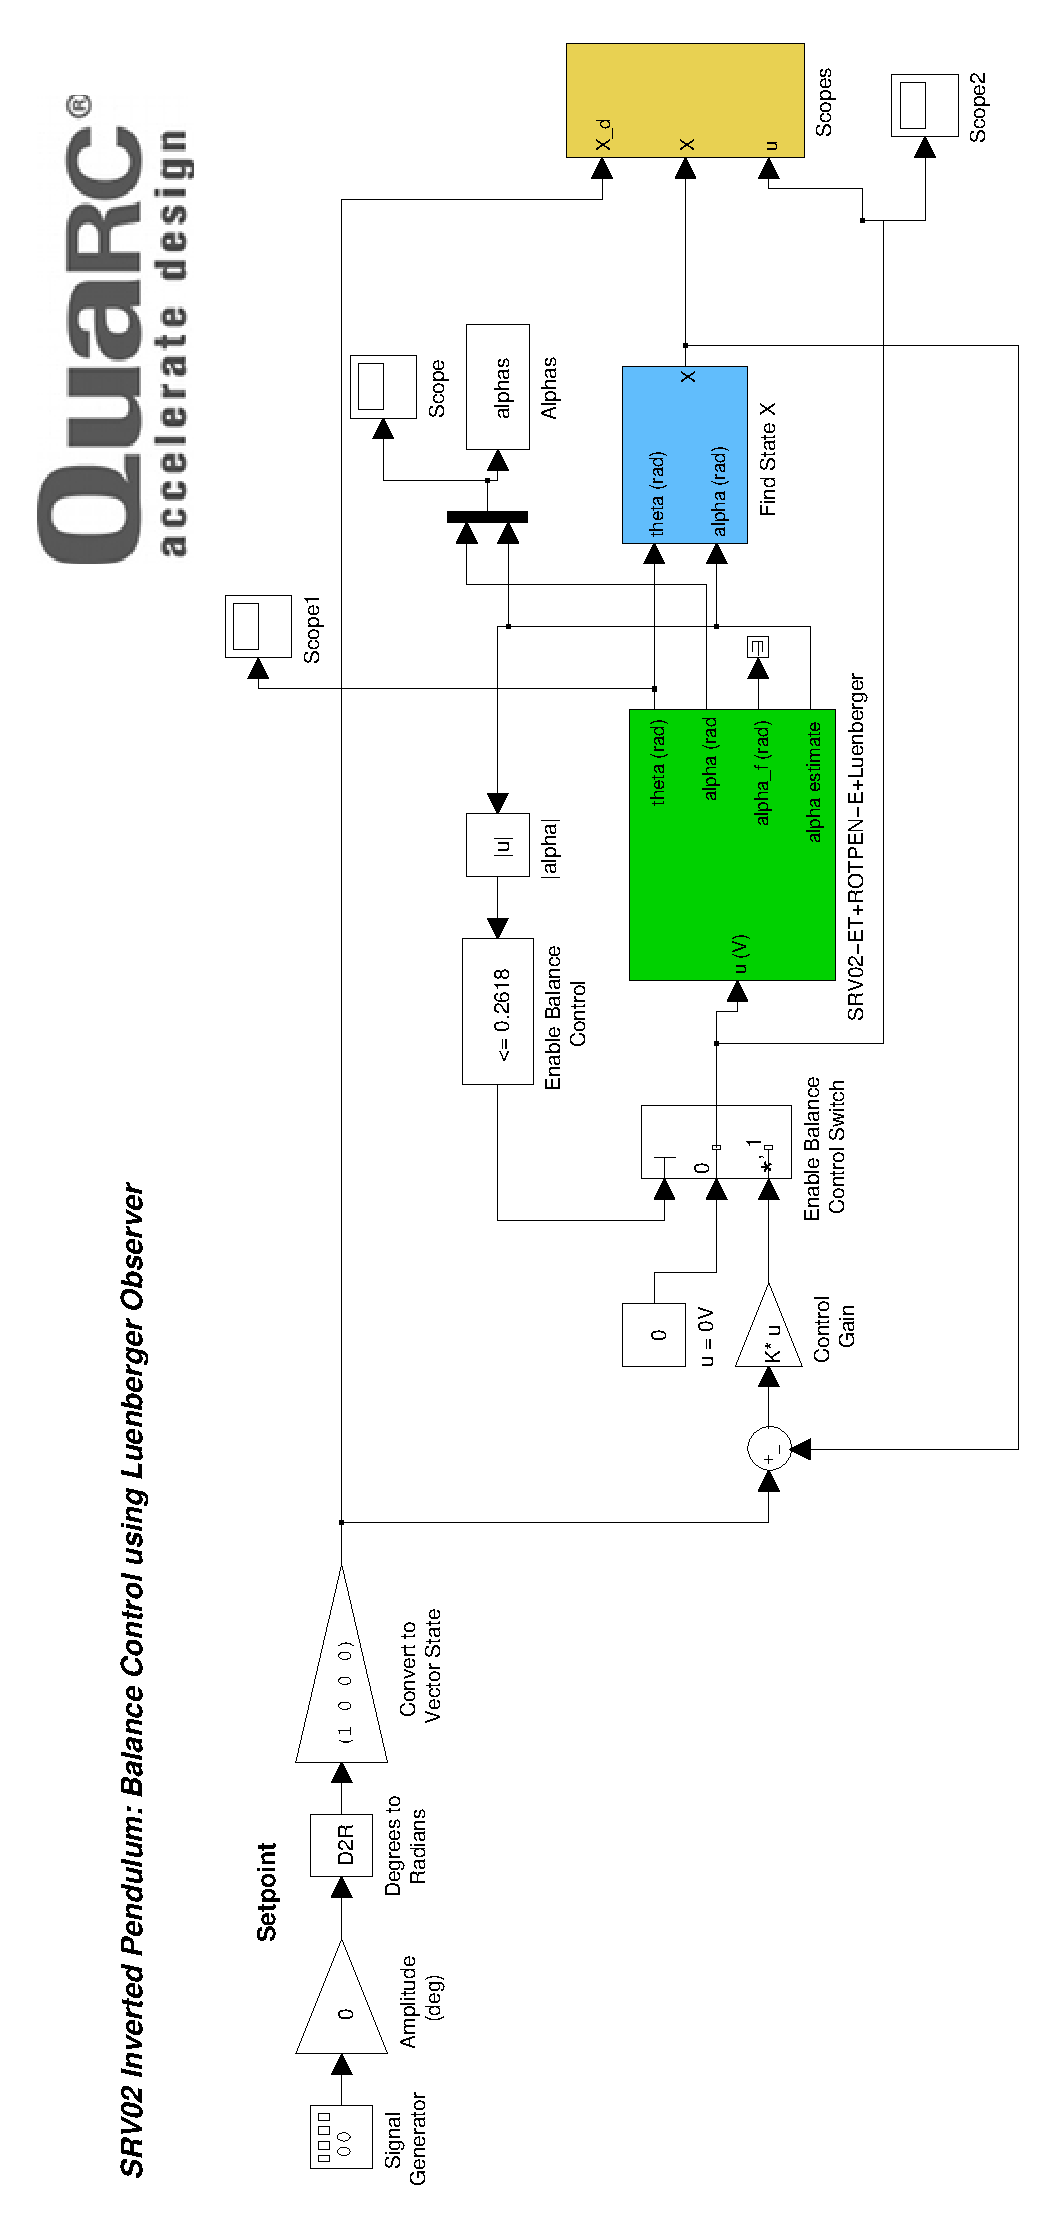
\includegraphics[width=0.5\textwidth,angle=-90]{eps/lab_3/balance_controller_luenberger}
          %\caption{A closed-loop feedback system for the rotary pendulum using partial state feedback and state estimate feedback.}
          %\end{figure}
          %
          %The nature of this experiment is to tune the observer gain, $L$, so that the state estimates are accurate enough to achieve balance control. To tune $L$, you should compare the measured pendulum angle and the estimated pendulum angle using a Scope block (to compare in real-time). After downloading the Simulink model to the target and pressing Run, you can lift the pendulum slightly, observe the error in the pendulum angle estimate via the Scope block, and tune the observer gain appropriately. You should start by setting the poles of $A-LC$ at five times more negative than the dominating pole among $\{-2.8 + 2.86i, \; -2.8 - 2.86i, \; -30, \; -40\}$. \textbf{Note:} you cannot have algebraic multiplicity greater than one when using the \emph{place} command, so you'll have to separate these poles by some numbers that you choose).
          %
          %Once your observer gain is properly tuned, you can lift up the pendulum to the inverted orientation and see if your control system can achieve balancing the pendulum.
          %
          %\begin{enumerate}[Questions]
          %\item[Q8:] First, plot your measured and your estimated pendulum angle with respect to time. Next, plot your control input with respect to time. Did your control system balance the inverted pendulum using partial state feedback and state estimate feedback? Where did you place the poles of your observer gain to achieve this balance control?\\
          %\drew{Answer: Yes, the control system managed to balance the inverted pendulum by using an observer gain of $L = \{-90,\; -92,\; -92.5,\; -93  \}$:
          %\begin{figure}[htb!]
          %\centering
          %\subfigure{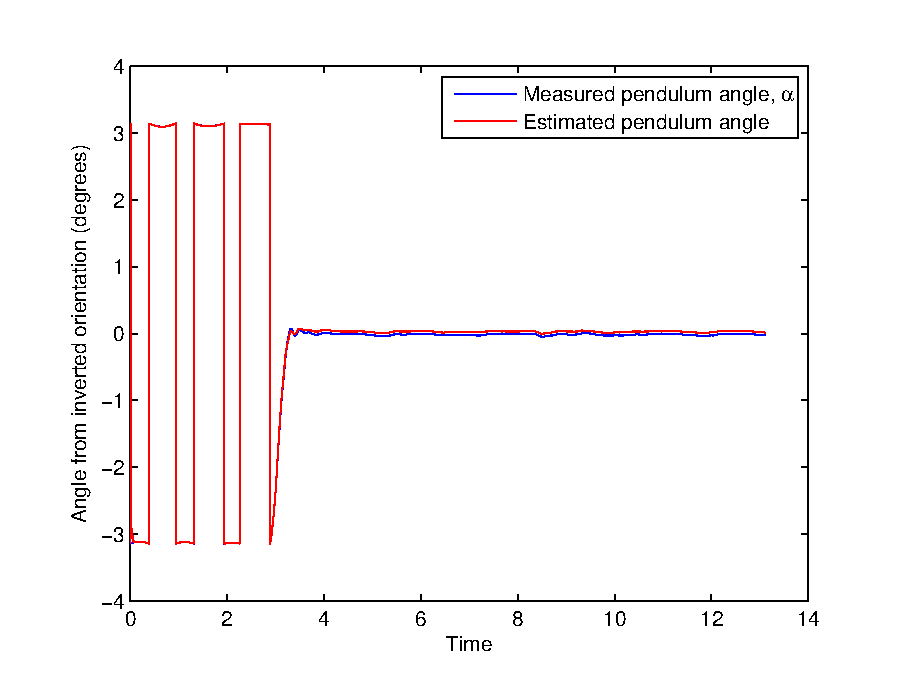
\includegraphics[width=0.5\linewidth]{eps/lab_3/luenberger_closed_loop_alphas}}
          %\subfigure{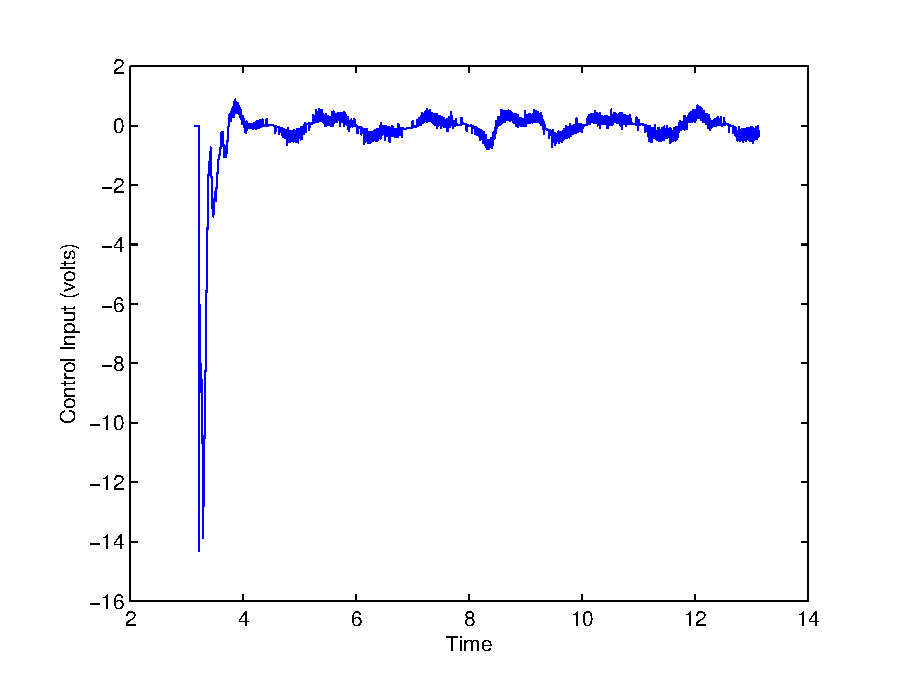
\includegraphics[width=0.5\linewidth]{eps/lab_3/luenberger_closed_loop_input}}
          %\caption{Plots of the estimated and measured pendulum angle, $\alpha$, and the control input. Note that the estimated and measured $\alpha$ agree very well, and one can observe that the control system does balance the inverted pendulum just past three seconds. The control input is constantly adjusting the rotor base to allow the pendulum to stay upright.}
          %\end{figure}}
          %\end{enumerate}
\end{enumerate}

When you have completed the lab, make sure you save your files in a convenient location (e.g.\ on some type of cloud storage).

\section{Deliverables}
Prepare a brief write up describing what you learned from this lab. This does not need to be a formal report, but all material should be presented in a clear and logical manner, with concise descriptions where necessary. Include your answers to all the questions in the lab (these are the lettered sections in the procedure), as well as any requested plots.
\chapter{Lab 4: LQR Optimization for Feedback Control and Observer Design for the Rotary Flexible Beam}

The purpose of this lab is to design and optimize a feedback controller for the rotary flexible beam system. One way of achieving this is to use a Linear Quadratic Regulator, which automates the process of finding a state feedback gain $K$ in a way that optimizes the system for certain design parameters. The prelab focuses on analyzing the stability of the open-loop rotary flexible beam system. In the lab, you will first design and optimize the closed-loop state feedback system by using the LQR technique to minimize the flexible beam's deflections while the rotor base tracks an input signal trajectory. The closed-loop system will have to adhere to set restrictions on settling time, percent overshoot and maximal flexible beam deflection. Next, you will observe the effects of using only partial state feedback on the system response to an input. Finally, you will attempt to minimize these system response effects by building an observer for the unobservable state and using the ensuing state estimate as feedback.
\begin{figure}[htb!]
    \centering
    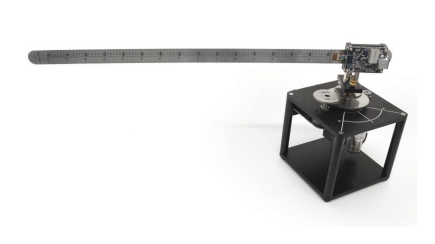
\includegraphics[width=.6\linewidth]{eps/lab_1/quanser.eps}
    \caption{Qanser SRV02 with flexible beam module~\cite{Q-Flex-Beam}.}
    \label{fig:lab4_plant}
\end{figure}

\section{Background Information}
\subsection{Modelling the Beam Using the Euler Lagrange Equation}
For now, we will study the simplest model of the rotary flexible beam - the 2-degree-of-freedom model. Thus, our two coordinates of interest are the rotation angle \( \theta \) and the deflection angle \( \alpha \). See below for what these coordinates look like in the physical system.
\begin{figure}[htb!]
    \centering
    \begin{subfigure}{.4\textwidth}
        \centering
        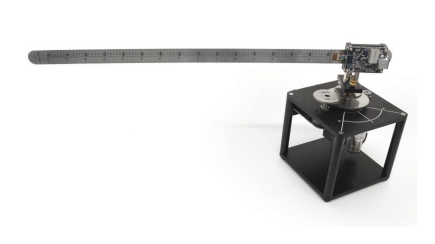
\includegraphics[width=\textwidth]{eps/lab_1/quanser.eps}
        \caption{}
    \end{subfigure}\hfill
    \begin{subfigure}{,4\textwidth}
        \centering
        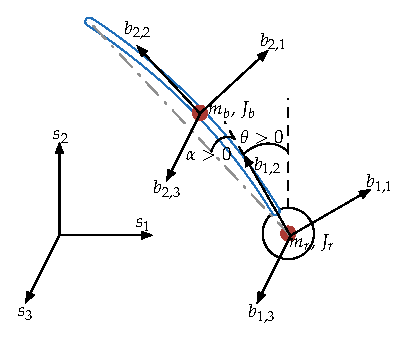
\includegraphics[width=\textwidth]{eps/lab_1/rotary_flexible_beam_edit.eps}
        \caption{}
    \end{subfigure}
    \caption{(a) Physical rotary flexible beam system~\cite{Q-Flex-Beam}; (b) top view of a 2-DOF model of the physical system with one flexible body and one rigid base, where the flexible body and the rotor base both rotate in the horizontal plane. The reference coordinate axes are shown by $\{s_1,s_2,s_3\}$, the rotor base coordinate axes are shown by $\{b_{1,1},b_{1,2}, b_{1,3}\}$, and the flexible body coordinate axes are shown by $\{b_{2,1},b_{2,2},b_{2,3}\}$. The centres of mass for both bodies are shown in red, and the rotation angle, $\theta$, and deflection angle of the beam's tip, $\alpha$, are shown.}
    \label{fig:lab1_rotary_flexible_beam}
\end{figure}

\subsubsection{Setting up the Rotary Flexible Beam}\label{sub subsection:lab1_setup}
The only thing you should have to do with the beam is to turn on the power amplifier. The power switch is located at the back of the amplifier (good luck finding it). Make sure to turn off the power amplifier before you leave the lab.See Appendix~\ref{chap:hardware} for more info on the configuration of the flexible beam.

\subsection{The LQ Problem}
A fundamental problem in control theory is operating a control system at minimum cost. When concerned with linear differential equations (e.g., $\mathbf{\dot{x}}(t) = A\mathbf{x}(t) + Bu(t)$) and quadratic cost functions, then one is really concerned with the \emph{LQ problem}. In this lab, we will use a main result from this area of literature~\cite{kwakernaak1972linear} which is the solution to the linear quadratic regulator (LQR). The solution to the LQR will help you design a feedback controller which minimizes the deflections of the flexible beam while the rotor base tracks a square wave trajectory (within certain \emph{design constraints} on settling time and overshoot).

The LQ problem that we are dealing with is an infinite-horizon problem that studies the control system
\[
    \begin{cases}
        \dot{\mathbf{x}}(t) = A\mathbf{x}(t)+Bu(t), \quad \text{where} \; \mathbf{x}(0) = \mathbf{x}_0 \\
        \mathbf{y}(t) = C \mathbf{x}(t)
    \end{cases}
\]
subject to minimizing the cost function
\[
    \eta(u) = \int_0^{\infty} \mathbf{y}^T(t)\mathbf{y}(t) + u^T(t)u(t) \; dt = \int_0^\infty  \mathbf{x}^T(t) C^T C \mathbf{x}(t) + u^T(t)u(t) \; dt.
\]
You may think of the first part of the cost function, $ \int_0^{\infty} \mathbf{y}^T(t)\mathbf{y}(t) dt$, as the \emph{energy of the controlled output}, and the second part, $\int_0^{\infty} u^T(t)u(t) dt$, as the \emph{energy of the control input}.

Two \textbf{main results} from class follow this reformulation: the first is that if $(A,B,C)$ is a minimal realization, then there exists a positive definite symmetric solution $\Pi_{\infty} \in \mathcal{M}^{n \times n}(\mathbb{R})$ to the continuous algebraic Ricatti equation (CARE):
\[
    A^T \Pi_{\infty} + \Pi_{\infty} A - \Pi_{\infty} B B^T \Pi_{\infty} = -C^T C;
\]
the next main result is that with $(A,B,C)$ a minimal realization, the controller
\[
    u(t) = -B^T \Pi_{\infty} \mathbf{x}(t)
\]
solves the LQ problem.

\subsection{Matrices}\label{section:lab4_prelab}
The following sections will provide relevant matrices/equations for the lab. Don't get too caught up in the calculations, just understand the rough ideas, and use the provided matrices/equations as required.

\subsection{Equations of Motion for the Rotary Flexible Beam}
In a similar fashion to Lab 3, one can find the EOMs for the rotary flexible beam using the Euler-Lagrange equation and get state space matrices from these. See Appendix~\ref{chap:EOMs} for the derivations.

\[
    A =
    \left[\begin{array}{c c c c}
            0 & 0       & 1      & 0 \\
            0 & 0       & 0      & 1 \\
            0 & 623.77  & -40.49 & 0 \\
            0 & -965.53 & 40.49  & 0
        \end{array}\right]
\]

\[
    B =
    \left[\begin{array}{c}
            0      \\
            0      \\
            61.775 \\
            -61.775
        \end{array}\right].
\]

And using the fact that \(y = Cx + Du\),

\[
    C =
    \left[\begin{array}{c c c c}
            1 & 0 & 0 & 0 \\
            0 & 1 & 0 & 0
        \end{array}\right]
\]

\[
    D =
    \left[\begin{array}{c}
            0 \\
            0
        \end{array}\right],
\]

We note that the open-loop poles (that is, the eigenvalues of \(A\)) are $\{0,\; -8.13+22.47i,\; -8.13-22.47i,\; -24.21\}$, and both the algebraic and geometric multiplicities are equal, thus the system is internally stable.

To verify whether we can use full state feedback to steer the system, one must compute the controllability matrix:
\[
    \mathcal{C}_{(A,B)} = \left[\begin{array}{c c c c}
            0      & 61.77    & -2501.26  & 62750.59   \\
            0      & -61.77   & 2501.26   & -41639.42  \\
            61.77  & -2501.26 & 62750.59  & -980692.86 \\
            -61.77 & 2501.26  & -41639.42 & 125861.00
        \end{array}\right]
\]
The system's controllability matrix has full rank, and hence the system is controllable. Thus, we can hope to use full state feedback and pole placement techniques to control the system.

\section{Procedure}
\begin{enumerate}

    \item \textbf{Designing Feedback using the Linear Quadratic Regulator}\label{section:lab4_lqr}

          \begin{enumerate}
              \item What does it mean to be a minimal realization? Is the state-space model of the rotary flexible beam system a minimal realization? Can one hope to use the LQR approach to optimize the feedback control inputs for the rotary flexible beam system?

                    %\drew{Answer: Given any transfer function, any state-space model that is both controllable and observable and has the same input-output behaviour as the transfer function is said to be a minimal realization. As was shown in Lab 1, the state-space model of the rotary flexible beam accurately describes the physical system; since the transfer function describes the input and output behaviour of the physical system, one can conclude that the state-space model has the same input-output behaviour as the transfer function. Furthermore, the observability matrix for the state-space model is
                    %\[
                    %\mathcal{O}_{(C,A)} = \left[\begin{array}{c c c c}
                    %1 & 0 & 0 & 0\\
                    %0 & 1 & 0 & 0\\
                    %0 & 0 & 1 & 0\\
                    %0 & 0 & 0 & 1\\
                    %0 & 623.77 & -40.49 & 0\\
                    %0 & -965.53 & 40.49 & 0\\
                    %0 & -25257.84 & 1639.61 & 623.77\\
                    %0 & 25257.84 & -1639.61 & -965.53
                    %\end{array}\right]
                    %\]
                    %which has full rank (see prelab for computation of $\mathcal{C}_{(A,B)}$, which also has full rank). Thus, $(A,B,C)$ is a minimal realization, and one can use the main results for LQR theory to optimize the feedback control inputs for the physical system. 
                    %}
                    \vspace{0.5em}
                    There are a few differences in the theory that you've learned from class and the treatment we will apply here. First, we wish to minimize some of the system's outputs more than others, e.g., our focus is on minimizing the flexible beam deflections. With this focus, we present a more generalized form of the quadratic cost function:
                    \begin{equation}\label{lab4_cost_function}
                        \eta(u) = \int_0^{\infty} \mathbf{x}^T(t) Q \mathbf{x}(t) + u^T(t)u(t) \; dt,
                    \end{equation}
                    where $Q$ is symmetric and $\mathbf{x}^T(t) Q \mathbf{x}(t) > 0$ for all $t$ (positive-definite). You will set the matrix $Q$ as a diagonal weighting matrix to assign different weights on the states within the cost function~\eqref{lab4_cost_function}. In turn, this will determine how the control input $u(t)$ will minimize the cost function $\eta(u)$, and thus the weightings of matrix $Q$ will have direct effects on the ensuing feedback gain, $K$. Hence, the LQR design process is really an iterative process: tune the diagonal weightings of $Q$, observe the effects, compare against the desired performance metrics, and repeat.

                    In the theory from class, one had to verify that $(A,B,C)$ was a minimal realization in order for $u(t)=-B^T \Pi_{\infty} \mathbf{x}(t)$ to solve the LQ problem. Using the generalized quadratic cost function in~\eqref{lab4_cost_function}, one must only verify that $(A,B)$ be stabilizable to ensure that this input solves the LQ problem. Can the LQR approach be used to optimize the feedback control inputs for the rotary flexible beam?
                    %\drew{Answer: stabilizability follows from the fact that the system is controllable (see previous answer for $\mathcal{C}_{(A,B)}$ computation).}

                    Open the Simulink model \textbf{lqr\_model.mdl}, shown in Figure~\ref{lab4_lqr_simulink}. Notice the presence of a high-gain observer, used to estimate the time derivatives of the signals $\theta$ and $\alpha$, as was discussed in Section~\ref{section:lab3_feedback} of Lab 3. In this lab, you will use these signal derivative estimates as feedback. Notice also that the output signal is subtracted from the input signal before being scaled by the feedback gain. Thus when the system's outputs match the system's inputs, a signal of all zeros will be input into the physical system; when the system inputs and outputs do not match, the feedback gain should be designed to drive the non-zero states to zero (this will work if $K$ is designed to make the closed-loop system \emph{asymptotically stable}).
                    \begin{figure}[htb!]
                        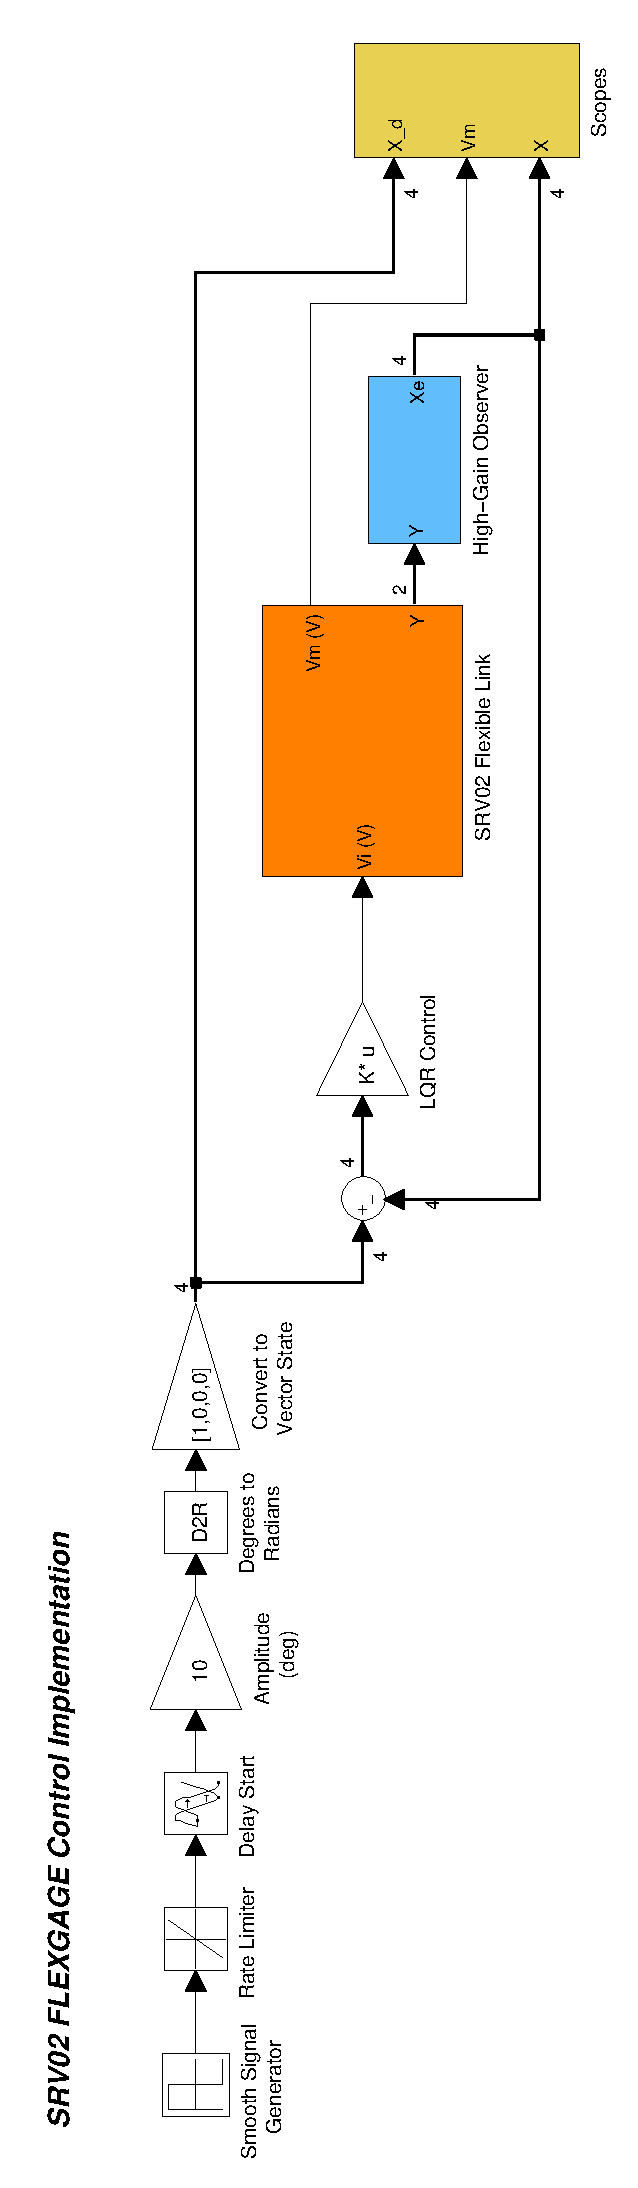
\includegraphics[width=0.3\linewidth,angle=-90]{eps/lab_4/lqr_simulink}
                        \caption{A Simulink model that inputs a signal into the rotary flexible beam system and observes its output. This model can be used to drive the rotor base to track a signal input while minimizing the flexible beam deflections via full state feedback. The feedback gain $K$ is designed using a linear quadratic regulator.}
                        \label{lab4_lqr_simulink}
                    \end{figure}

                    Your first task will be to observe the effects of changing the diagonal weightings of $Q$. Using your state-space matrices from Section~\ref{section:lab4_prelab}, and setting
                    \[
                        Q = \left[\begin{array}{c c c c}
                                q_1 & 0   & 0   & 0   \\
                                0   & q_2 & 0   & 0   \\
                                0   & 0   & q_3 & 0   \\
                                0   & 0   & 0   & q_4
                            \end{array}\right]
                    \]
                    you can use the MATLAB command \emph{care} to solve the continuous algebraic Ricatti equation (CARE). This will return the solutions to the Riccati equation, $\Pi_{\infty}$, which you will use to compute your feedback gain, $K=-B^T \Pi_{\infty}$.
              \item Using a diagonal weightings matrix for $Q$, express the cost function symbolically. What would be the effect of increasing the diagonal elements $q_i$ on the feedback gain, $K$?
                    %\drew{Answer:
                    %\begin{align*}
                    %\eta(u) &= \bigint_0^{\infty} \left( [\theta \quad \alpha \quad \dot{\theta} \quad \dot{\alpha}] \left[\begin{array}{c c c c} 
                    %q_1 & 0 & 0 & 0\\
                    %0 & q_2 & 0 & 0\\
                    %0 & 0 & q_3 & 0\\
                    %0 & 0 & 0 & q_4
                    %\end{array}\right] \left[\begin{array}{c} \theta \\ \alpha \\ \dot{\theta} \\ \dot{\alpha} \end{array}\right] + u^T(t)u(t) \right)\; dt \\
                    %& = \int_0^{\infty} q_1\theta^2 + q_2\alpha^2 + q_3\dot{\theta}^2 + q_4\dot{\alpha}^2 +u^2(t) \; dt
                    %\end{align*}
                    %Increasing the weightings $q_i$ would alter the cost function so as to give the corresponding state more influence over the cost, e.g., increasing $q_1$ would cause the control input $u(t)$ to have a bias towards minimizing the state scaled by $q_1$ (in our lab, this state is $\theta$), and thus would increase the corresponding feedback gain element $k_1$ to compensate, where
                    %\[
                    %K = \left[\begin{array}{c} k_1 \\ k_2 \\ k_3 \\ k_4 \end{array}\right].
                    %\]
                    %This behaviour is the same for all weightings $q_i$. Note that due to the interconnectedness of the system states, changing one $q_i$ may (and usually will) effect multiple states.
                    %}
              \item \emph{Check your feedback gain with your TA}. Since the Simulink model \emph{subtracts} the feedback from the input, make sure you define $K$ as $K=B^T \Pi_{\infty}$ and \textbf{not} $-K=B^T \Pi_{\infty}$. Vary the weightings $q_1,\; q_2,\; q_3,\; q_4$ independently from starting values $[q_1,\; q_2,\; q_3,\; q_4] = [1,\; 1,\; 1,\; 1]$. Run \textbf{lqr\_model.mdl} with a square wave input of amplitude 30 \textbf{total} (there is a signal amplitude \& an amplitude block, multiply these to get 30) and with frequency of 0.33 Hz. What effects does each modification have on the feedback gain, $K = [k_1,\; k_2,\; k_3,\; k_4]$? Plot each of the state responses with respect to time. What effects does each modification have on the physical system's state responses? What weighting(s) has(have) noticeable effects on reducing the rise time (one in particular is noticeable)? Did any decrease the flexible beam's deflections? \emph{Formulate problems and their specifications} that you anticipate when tuning particular weightings in various \emph{engineering applications} (e.g., for tidal power generators - or flexible beams mounted on the ocean floor in locations of notably strong tidal power - where the flexible beam's deflections trigger a power generator, but can also be strained to failure).
                    %\drew{Answer: Here are the plots and the corresponding feedback gains produced by the linear quadratic regulator:
                    %\begin{figure}[htb!]
                    %\subfigure{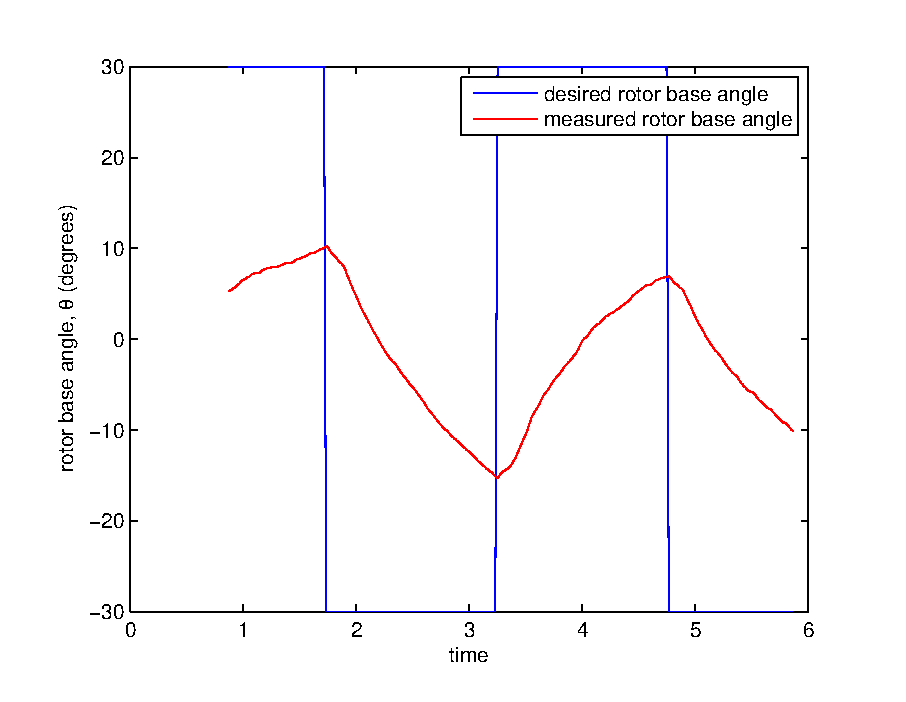
\includegraphics[width=0.5\linewidth]{eps/lab_4/theta_q_1_1_1_1}}
                    %\subfigure{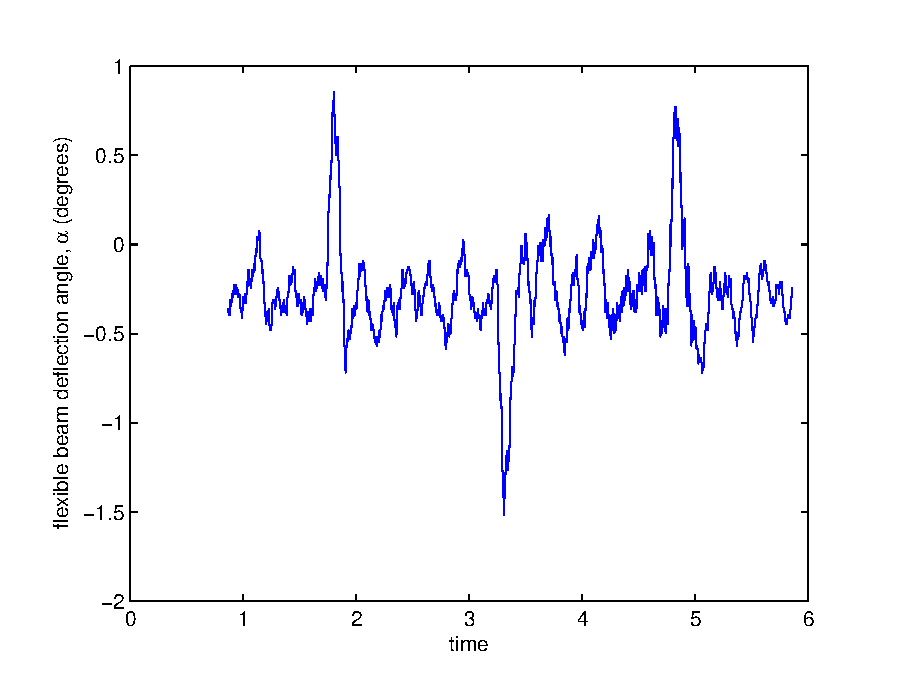
\includegraphics[width=0.5\linewidth]{eps/lab_4/alpha_q_1_1_1_1}}
                    %\caption{a) The rotor base response to a square wave input when $[q_1,\; q_2,\; q_3,\; q_4] = [1,\; 1,\; 1,\; 1]$, giving $[k_1,\; k_2,\; k_3,\; k_4] = [1,\; -9.5873,\; 0.6004,\; -0.4092]$, and b) the corresponding flexible beam deflection angle with respect to time.}
                    %\end{figure}
                    %\begin{figure}[htb!]
                    %\subfigure{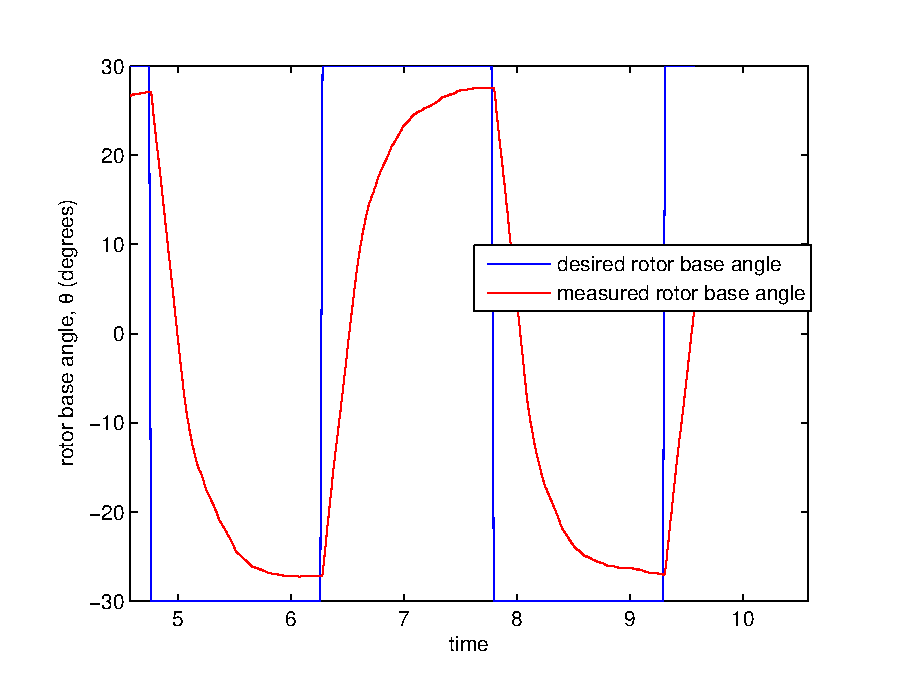
\includegraphics[width=0.5\linewidth]{eps/lab_4/theta_q_20_1_1_1}}
                    %\subfigure{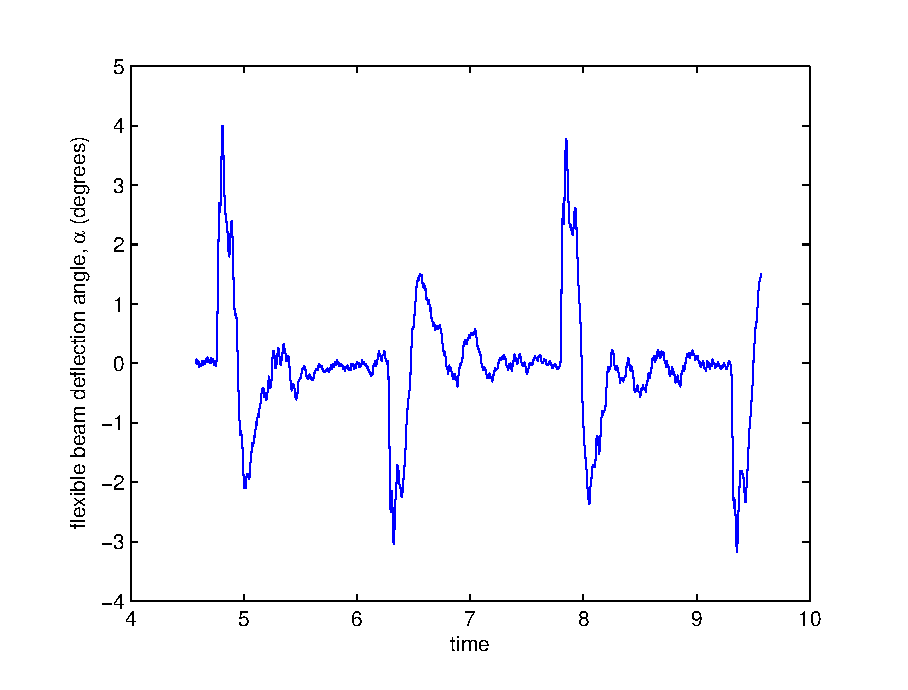
\includegraphics[width=0.5\linewidth]{eps/lab_4/alpha_q_20_1_1_1}}
                    %\caption{a) The rotor base response to a square wave input when $[q_1,\; q_2,\; q_3,\; q_4] = [20,\; 1,\; 1,\; 1]$, giving $[k_1,\; k_2,\; k_3,\; k_4] = [4.4721,\; -10.464,\; 0.798,\; -0.253]$, and b) the corresponding flexible beam deflection angle with respect to time.}
                    %\end{figure}
                    %\begin{figure}[htb!]
                    %\subfigure{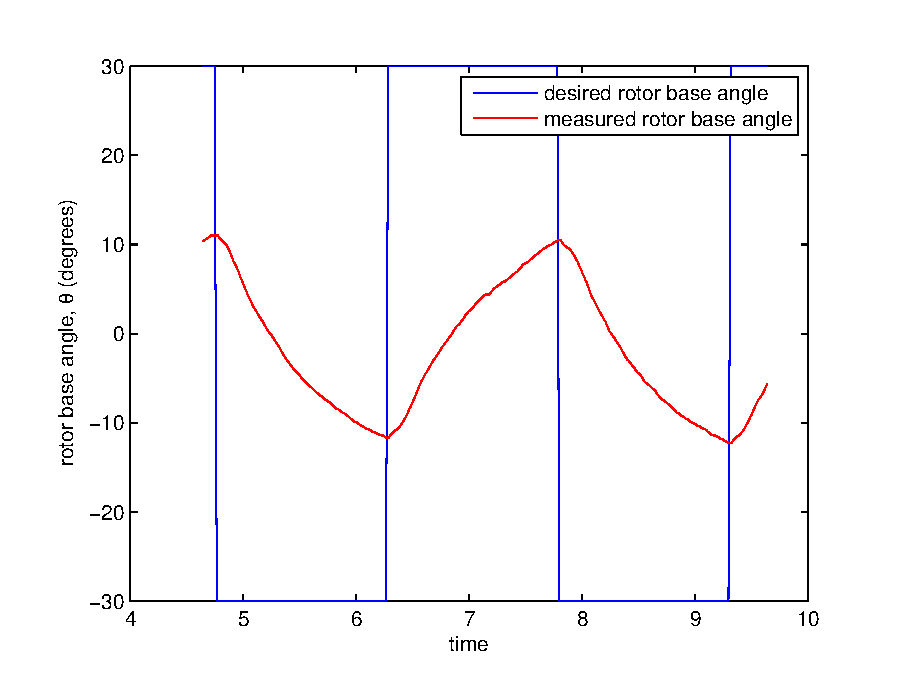
\includegraphics[width=0.5\linewidth]{eps/lab_4/theta_q_1_20_1_1}}
                    %\subfigure{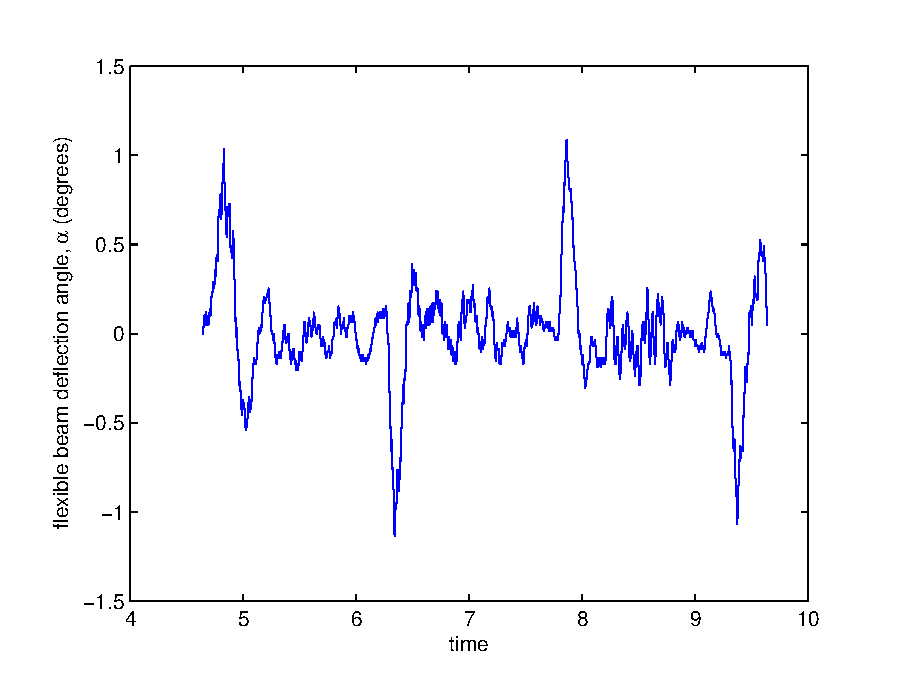
\includegraphics[width=0.5\linewidth]{eps/lab_4/alpha_q_1_20_1_1}}
                    %\caption{a) The rotor base response to a square wave input when $[q_1,\; q_2,\; q_3,\; q_4] = [1,\; 20,\; 1,\; 1]$, giving $[k_1,\; k_2,\; k_3,\; k_4] = [1,\; -10.408,\; 0.601,\; -0.413]$, and b) the corresponding flexible beam deflection angle with respect to time.}
                    %\end{figure}
                    %\begin{figure}[htb!]
                    %\subfigure{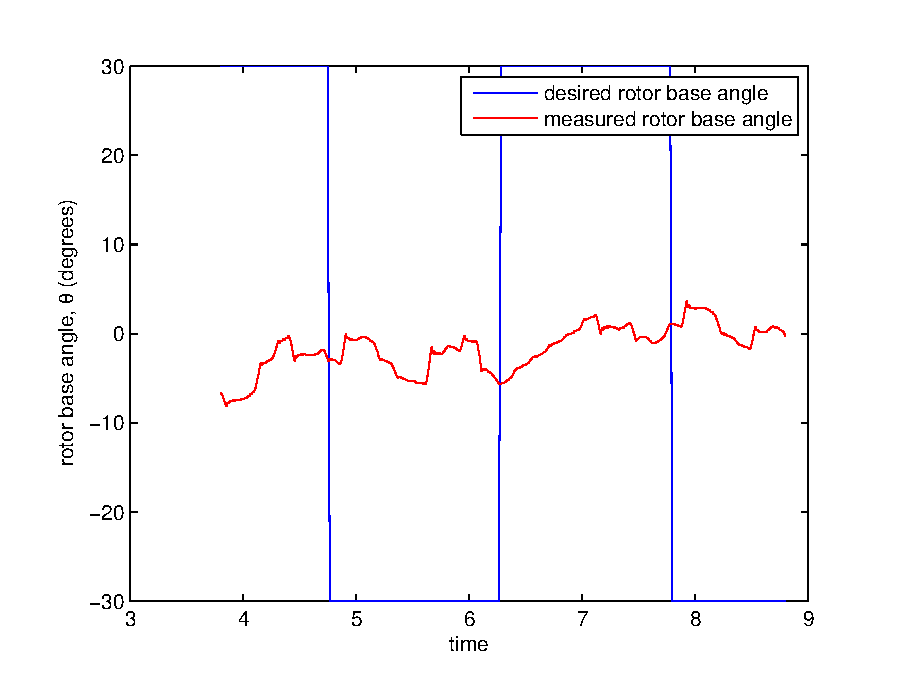
\includegraphics[width=0.5\linewidth]{eps/lab_4/theta_q_1_1_20_1}}
                    %\subfigure{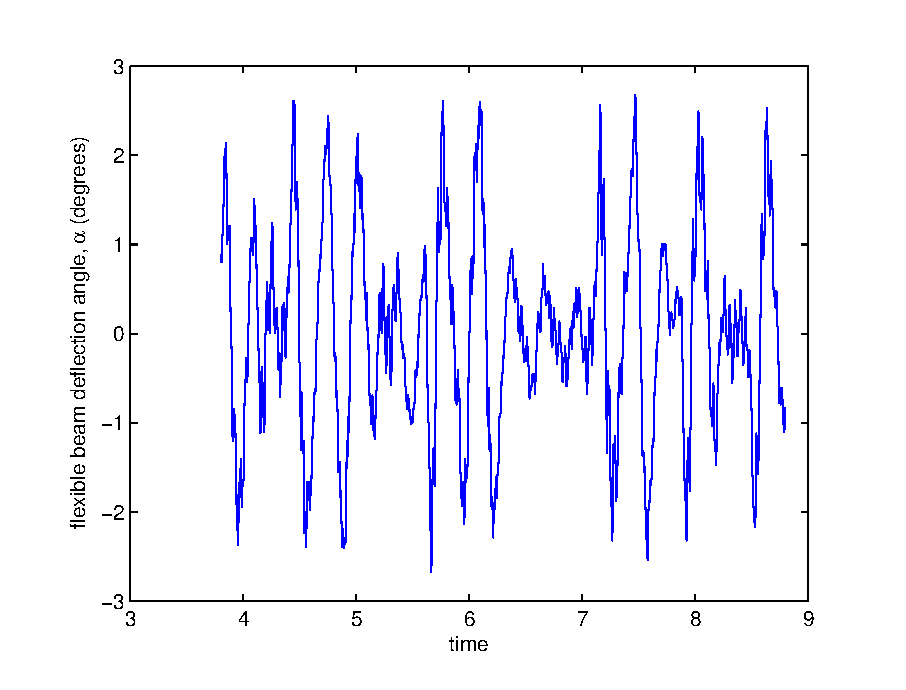
\includegraphics[width=0.5\linewidth]{eps/lab_4/alpha_q_1_1_20_1}}
                    %\caption{a) The rotor base response to a square wave input when $[q_1,\; q_2,\; q_3,\; q_4] = [1,\; 1,\; 20,\; 1]$, giving $[k_1,\; k_2,\; k_3,\; k_4] = [1,\; -10.85,\; 3.881,\; -0.133]$, and b) the corresponding flexible beam deflection angle with respect to time.}
                    %\end{figure}
                    %\begin{figure}[htb!]
                    %\subfigure{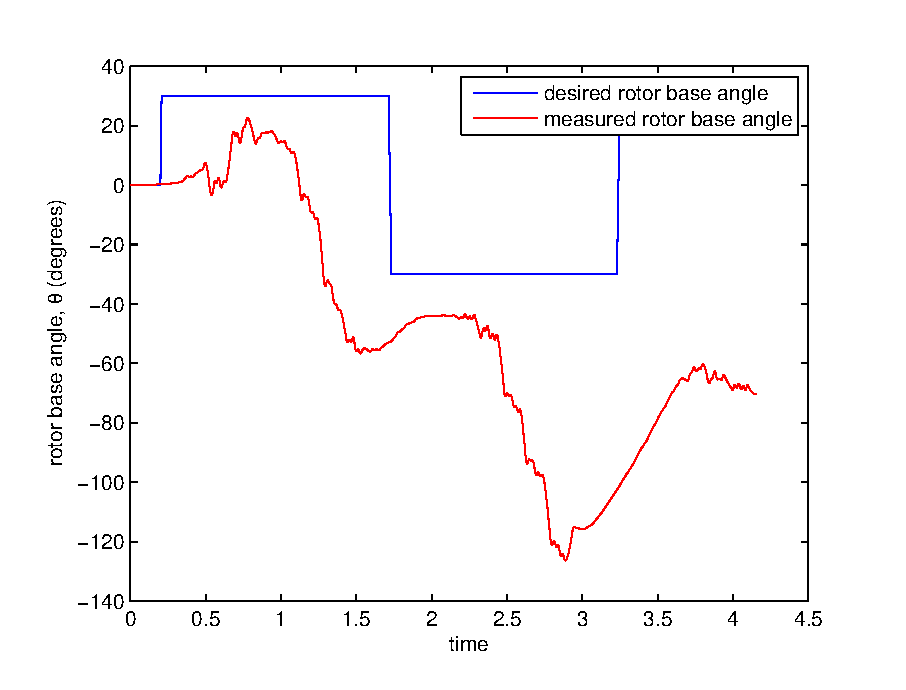
\includegraphics[width=0.5\linewidth]{eps/lab_4/theta_q_1_1_1_20}}
                    %\subfigure{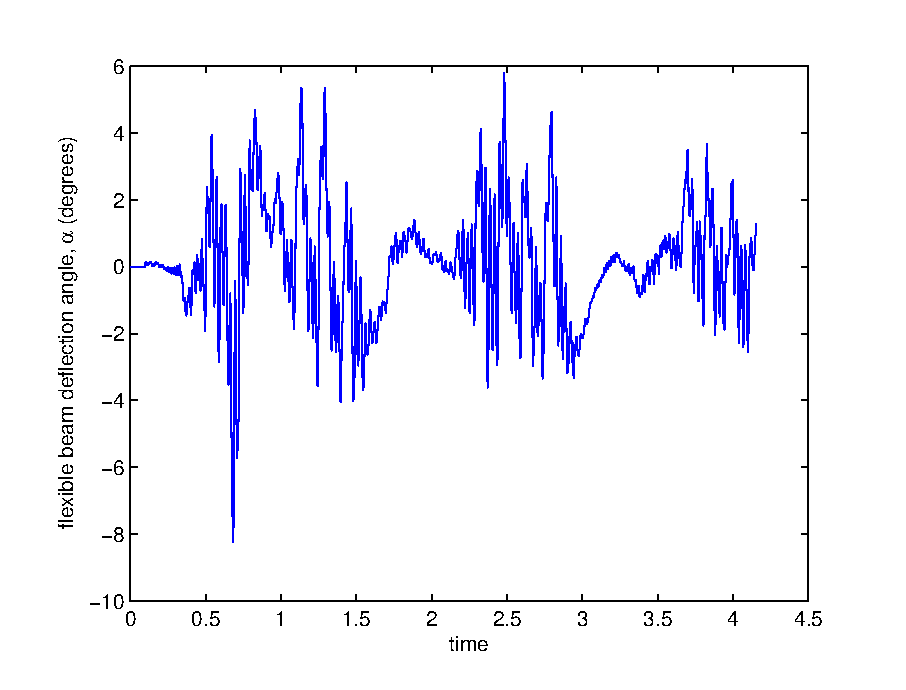
\includegraphics[width=0.5\linewidth]{eps/lab_4/alpha_q_1_1_1_20}}
                    %\caption{a) The rotor base response to a square wave input when $[q_1,\; q_2,\; q_3,\; q_4] = [1,\; 1,\; 1,\; 20]$, giving $[k_1,\; k_2,\; k_3,\; k_4] = [1,\; -43.48,\; 0.677,\; -3.449]$, and b) the corresponding flexible beam deflection angle with respect to time.}
                    %\end{figure}}

                    %\clearpage
                    %\drew{One will notice that increasing $q_1$ has an impact on changing $k_1$, and that the rotor base response is much faster (rise time and settling time is decreased). Also, increasing $q_4$ has a large impact on changing $k_4$, and thus from a theoretical standpoint, the angular velocity of the flexible beam should be reduced by increasing $q_4$. The other weightings, $q_2$ and $q_3$, have little effect on the system.
                    %}
              \item You will perform a similar experiment with the same input (square wave with amplitude of 30 and frequency of 0.33$Hz$), except now there are \emph{design restrictions} on the rotor base's response: we require that maximum percent overshoot to be 10\%, the rise time be within 0.5 seconds and the steady-state error be within 5\% for use in our application. In addition, the maximum flexible beam deflection should be no more than \(10^o\). Tune the diagonal weightings of $Q$ until you've achieved the desired results, and then plot the rotor's base angle, $\theta$, and the flexible beam's deflection angle, $\alpha$, with respect to time. Also plot the control input with respect to time. What weightings in the matrix $Q$ did you use to achieve these results, and what was the resulting feedback gain, $K$?
                    %\drew{Answer: The weightings that were used to achieve the desired performance was $[q_1,\; q_2,\; q_3,\; q_4] = [130,\; 1,\; 1,\; 3.5]$, giving $[k_1,\; k_2,\; k_3,\; k_4] = [11.401,\; -25.031,\; 1.379,\; -0.436]$. Instructors should note that there can be large variances between flexible beam modules, so these answers should be marked correct not by whether students can replicate the same weightings but by whether they can achieve that achieve the required response characteristics. Here are the plots:
                    %\begin{figure}[htb!]
                    %\center{
                    %\subfigure{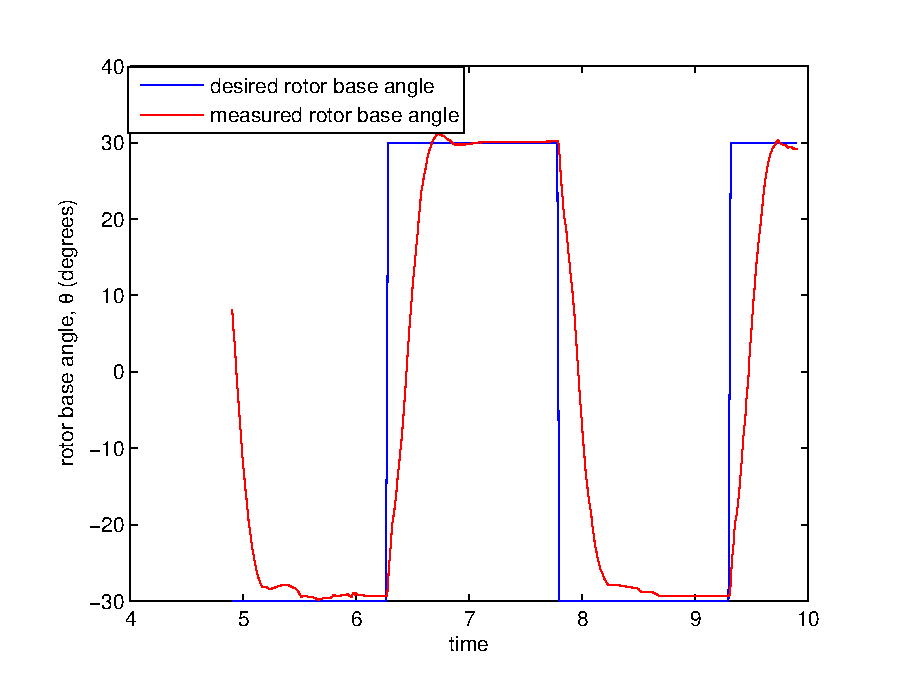
\includegraphics[width=0.4\linewidth]{eps/lab_4/theta_q_130_1_1_3half}}
                    %\subfigure{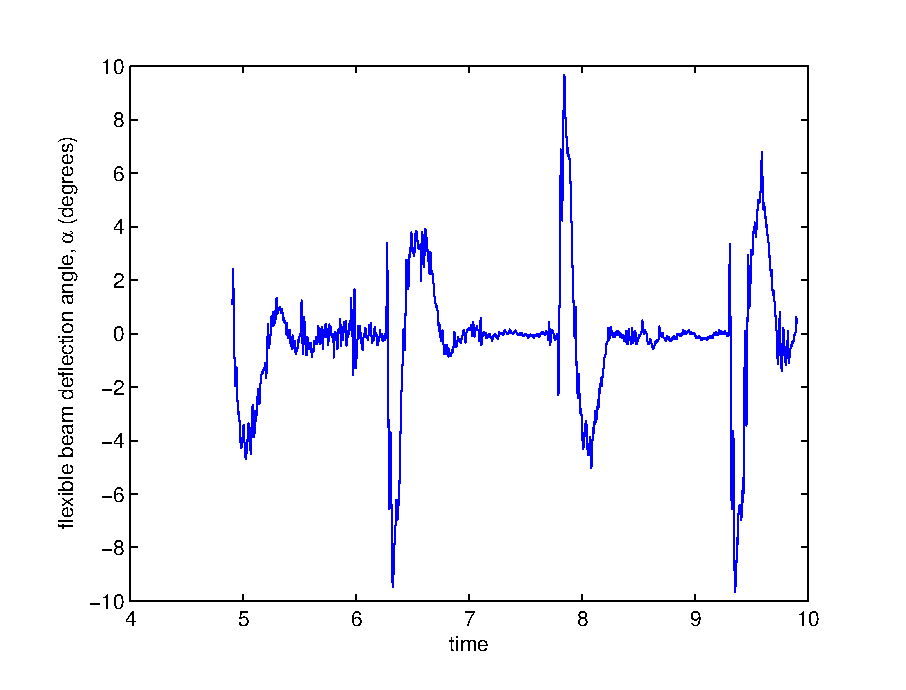
\includegraphics[width=0.4\linewidth]{eps/lab_4/alpha_q_130_1_1_3half}}
                    %\subfigure{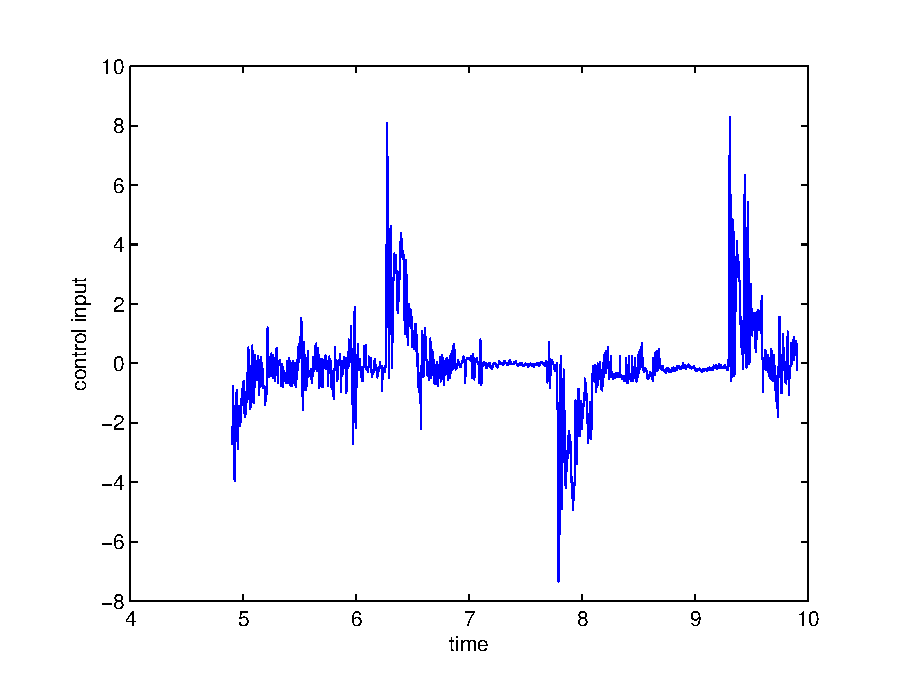
\includegraphics[width=0.4\linewidth]{eps/lab_4/vm_q_130_1_1_3half}}}
                    %\caption{a) The rotor base angle, and (b) the flexible beam deflection angle responses to a square wave input, with matrix $Q$ tuned to achieve the desired performance metrics.}
                    %\end{figure}
                    %}
          \end{enumerate}
    \item \textbf{Effects of Partial State Feedback on LQR}\label{subsection:lab4_partial_feedback}

          Now, you will observe the effects of using only partial state feedback in your closed-loop system on the optimality of the control system. Open the Simulink model \textbf{lqr\_partial\_feedback\_model.mdl}. Notice that the only state feedback being used is $\theta$ and the high-gain observer estimate of $\dot{\theta}$, as shown in Figure~\ref{lab4_lqr_partial_simulink}.
          \begin{figure}[htb!]
              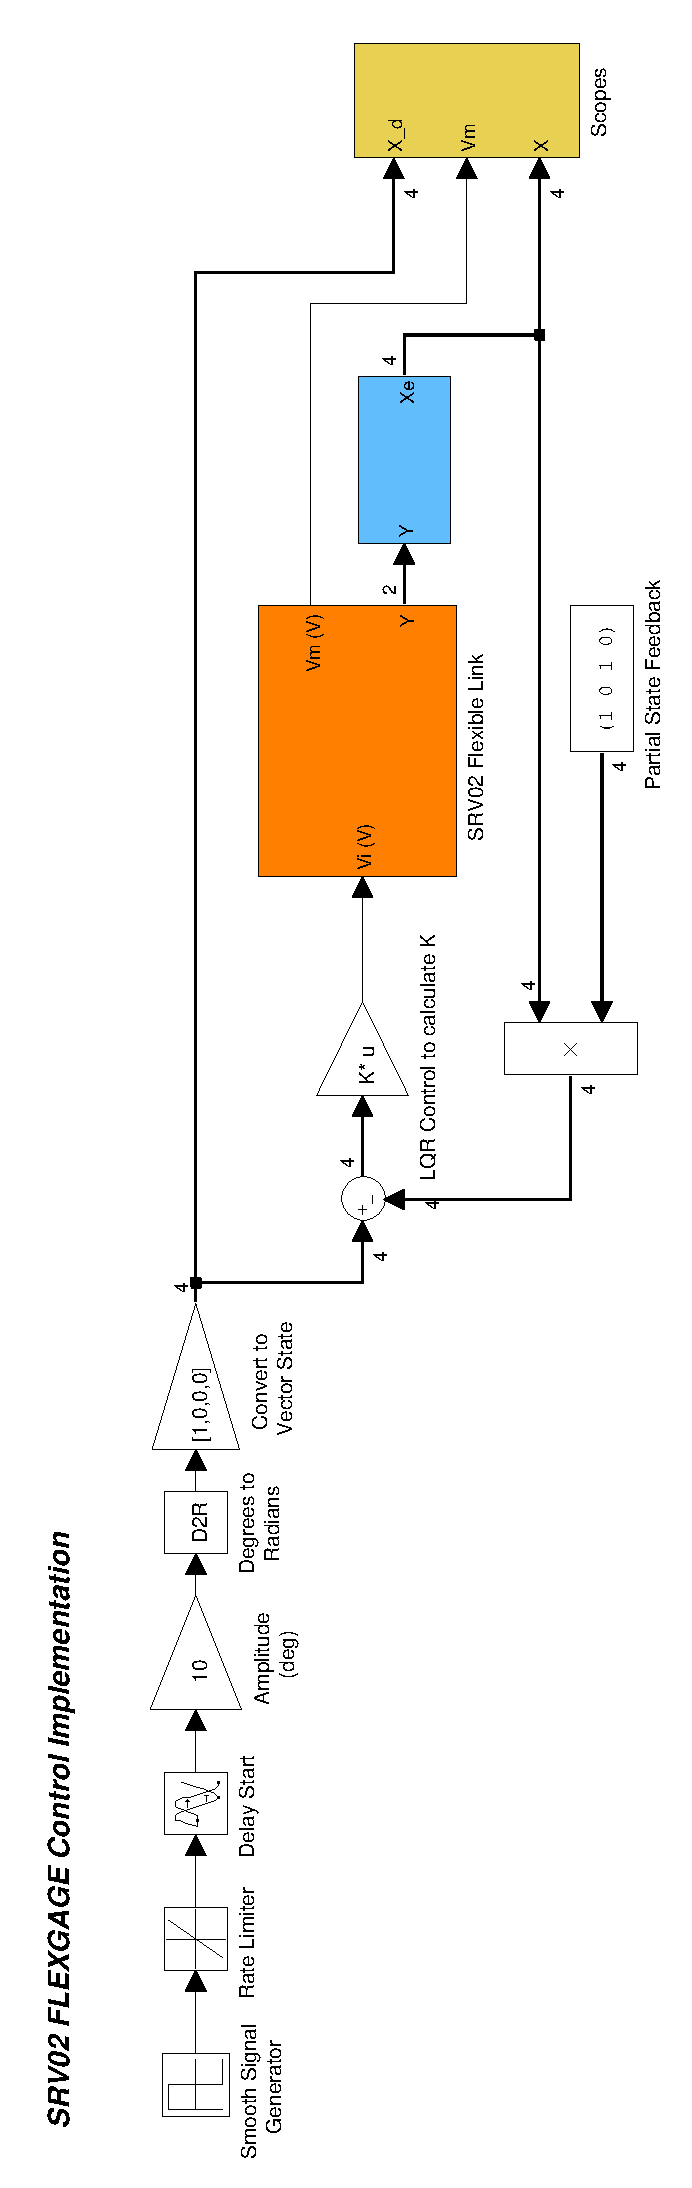
\includegraphics[width=0.3\linewidth,angle=-90]{eps/lab_4/lqr_partial_feedback_simulink}
              \caption{A Simulink model of the rotary flexible beam that utilizes partial state feedback and the linear quadratic regulator to design a feedback gain, $K$, that minimizes the deflections of the flexible beam while the rotor base tracks a square wave trajectory.}
              \label{lab4_lqr_partial_simulink}
          \end{figure}

          \begin{enumerate}
              \item Similar to the last experiment, use the LQR technique and the same weighting matrix $Q$ when computing your feedback gain, $K$. Plot the system responses to a square wave function with amplitude 30 and with frequency of 0.33 Hz. Compare the optimality of full state feedback and the partial state feedback closed-loop systems. Describe at least two previously-learned techniques that you may employ (and describe how) to obtain a better state feedback design, leading to superior system behaviour.
                    %\drew{Answer: in the partial state feedback case, the closed-loop control system is less optimal than the full state feedback system: the beam deflects much more and the steady-state error is higher. Due to the design of the cost function, these increases in beam deflection and steady-state error result in a higher cost. The control input is slightly less, but due to the design of the cost function, this will lower the cost significantly.
                    %\begin{figure}[htb!]
                    %\subfigure{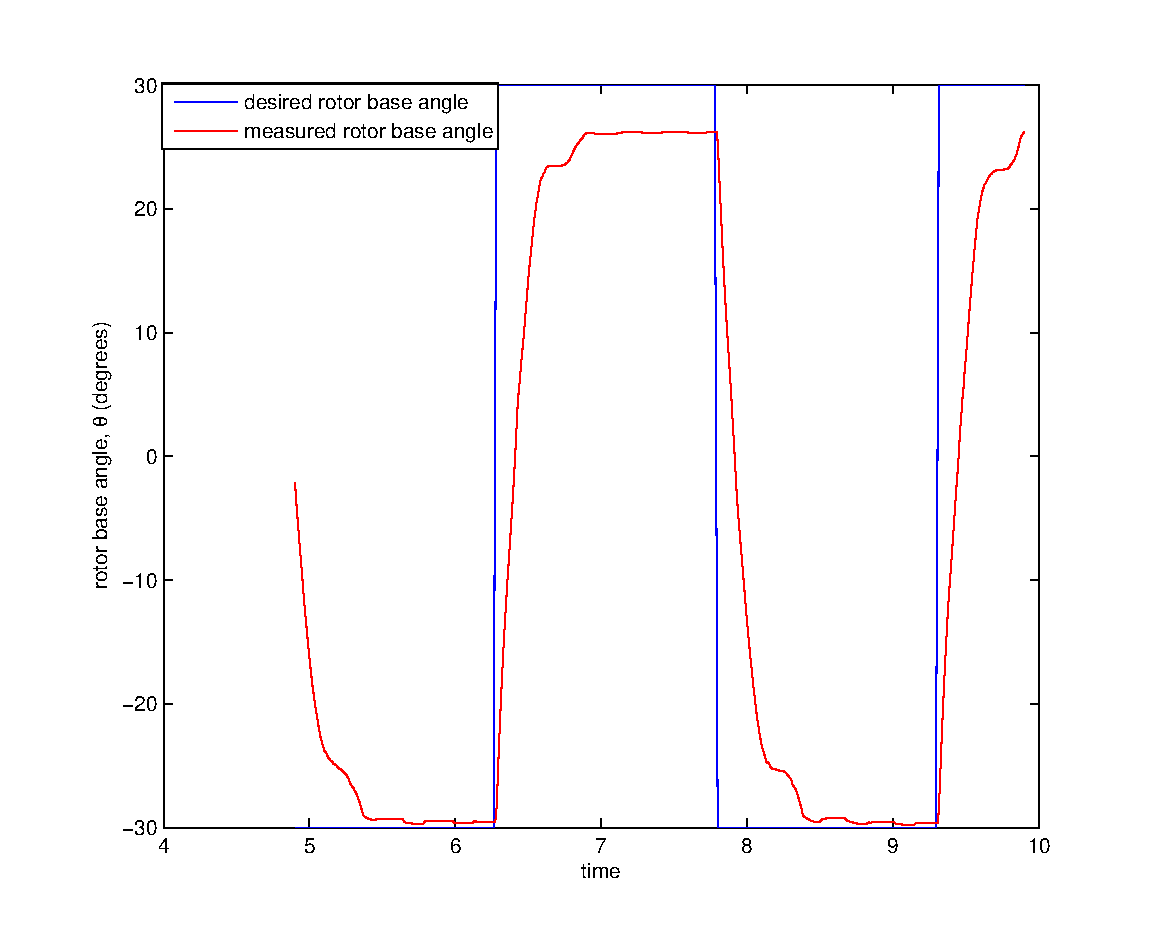
\includegraphics[width=0.48\linewidth]{eps/lab_4/theta_q_130_1_1_3half_partial}}
                    %\subfigure{\includegraphics[width=0.5\linewidth]{eps/lab_4/alpha_q_130_1_1_3half_partial}}
                    %\center{
                    %\subfigure{\includegraphics[width=0.5\linewidth]{eps/lab_4/vm_q_130_1_1_3half_partial}}}
                    %\caption{a) The rotor base angle, and (b) the flexible beam deflection angle responses to a square wave input when using only partial state feedback. This partial state feedback control system is less optimal than the full state feedback control system.}
                    %\end{figure}
                    %}
          \end{enumerate}

    \item \textbf{Designing an Observer \& Using Observer Estimate as Feedback for LQ Problem}\label{section:lab4_observer_lqr}
          \begin{enumerate}
              \item Is it possible to construct an observer for the rotary flexible link system, for the scenario where the strain gauge, which reads the flexible beam's deflection angle, is damaged?
                    %\drew{Answer: with this modification, the state-space matrix $C$ becomes
                    %\[
                    %C = \left[\begin{array}{c c c c}
                    %1 & 0 & 0 & 0\\
                    %0 & 0 & 0 & 0
                    %\end{array}\right]
                    %\]
                    %and the observability matrix becomes
                    %\[
                    %\mathcal{O}_{(A,C)} = \left[\begin{array}{c c c c}
                    %1 & 0 & 0 & 0\\
                    %0 & 0 & 0 & 0\\
                    %0 & 0 & 1 & 0\\
                    %0 & 0 & 0 & 0\\
                    %0 & 623.77 & -40.49 & 0\\
                    %0 & 0 & 0 & 0\\
                    %0 & -25257.84 & 1639.61 & 623.77\\
                    %0 & 0 & 0 & 0
                    %\end{array}\right]
                    %\]
                    %which has full rank. The controllability matrix does not change. Thus the modified system is controllable and observable, which implies that it is detectable and stabilizable. Hence, one can hope to construct an observer for the state $\alpha$, and then use the high-gain observer subsystem block to estimate $\dot{\alpha}$.}
          \end{enumerate}

          \begin{figure}[htb!]
              \centering
              \includegraphics[width=0.6\linewidth,angle=-90]{eps/lab_4/lqr_observer_model}
              \caption{A Simulink subsystem block showing the rotary pendulum system and a Luenberger observer. These systems are not connected, however one can connect these in such a way to compare the measured and estimated pendulum angle, $\alpha$ and $\hat{\alpha}$, as well as use the pendulum angle estimate as LQR feedback. Note that this model will not run without modification.}
              \label{figure:lab4_lqr_observer_model}
          \end{figure}
          \newpage
          \begin{enumerate}
              \item Open the Simulink model \textbf{lqr\_observer\_model} with the Luenberger observer contained in the rotary pendulum's subsystem block, as shown in Figure~\ref{figure:lab4_lqr_observer_model}. Follow the procedure from Section~\ref{section:lab3_observer} of Lab 3 to build a Luenberger state observer to estimate state $\alpha$. You will need to tune your observer gain, $L$, similarly to how you did so in Lab 3 so that the observer dynamics are faster than the system dynamics. However, now your feedback gain $K$ is being produced by the linear quadratic regulator, so tuning $Q$ will alter $K$ and thus the observer gain $L$ may have to be tuned concurrently. \textbf{Make sure} to change your output matrix, $C$, such that $\alpha$ is not an output. Use the estimate of the beam's deflection angle, $\hat{\alpha}$, to calculate an estimate for the angular velocity of the beam via the high-gain observer subsystem. Plot the responses of the rotor base angle and the flexible beam deflection angle due to a square wave input of amplitude 30 and frequency 0.33Hz. On the flexible beam deflection angle plot, also plot your state estimate (you'll need to use a To Workspace block for this). What are your gains $L$ and $K$ and what is your weighting matrix $Q$? What can you conclude about the optimality (i.e., rotor base trajectory tracking and beam's deflections) of this control system when comparing it to the partial state feedback scenario and the full state feedback scenario?
                    %\drew{Answer: with $Q$ weightings of $[q_1,\; q_2,\; q_3,\; q_4] = [130,\; 1,\; 1,\; 3.5]$, the resulting feedback gain weightings are $[k_1,\; k_2,\; k_3,\; k_4] = [11.401,\; -25.031,\; 1.379,\; -0.436]$. The observer gain weightings are $[l_1,\; l_2,\; l_3,\; l_4] = [-40,\; -41,\; -42,\; -43]$. The plots below reveal that the state estimate, $\hat{\alpha}$, and $\alpha$ agree pretty well. As a result of using partial state feedback and state estimate feedback, the magnitude of the flexible beam deflections is reduced throughout in comparison to the partial state feedback closed-loop system. In comparison to the full state feedback system, the overall flexible beam deflections are greater, and the rotor angle response is almost the same. The control input for the state estimate feedback system is slightly less than that for the full state feedback system, although this decrease is only weighted by 1 in the cost function, whereas beam deflection is weighted by 3.5. Thus using the state estimates as feedback is a more optimal control system than using only partial feedback, but not as optimal as using full state feedback (as is expected).
                    %\begin{figure}[htb!]
                    %\subfigure{\includegraphics[width=0.5\linewidth]{eps/lab_4/theta_observer_feedback}}
                    %\subfigure{\includegraphics[width=0.5\linewidth]{eps/lab_4/alpha_observer_feedback}}
                    %\center{
                    %\subfigure{\includegraphics[width=0.5\linewidth]{eps/lab_4/vm_observer_feedback}}
                    %\caption{a) The rotor base angle, and (b) the flexible beam deflection angle responses to a square wave input when using partial state feedback $\theta$, $\dot{\theta}$ and state estimate feedback, $\hat{\alpha}$, $\hat{\dot{\alpha}}$. This control system is less optimal than the full state feedback control system, but more optimal than the partial state feedback system.}}
                    %\end{figure}
                    %}
          \end{enumerate}
\end{enumerate}

When you have completed the lab, make sure you save your files in a convenient location (e.g.\ on some type of cloud storage).

\section{Deliverables}
Prepare a brief write up describing what you learned from this lab. This does not need to be a formal report, but all material should be presented in a clear and logical manner, with concise descriptions where necessary. Include your answers to all the questions in the lab (these are the lettered sections in the procedure), as well as any requested plots.

\appendix
\chapter{Matlab}\label{chap:MATLAB}

The students of this course should be familiar with the basic ideas of
computer programming and Matlab from first year courses.

\section{Defining variables}

\begin{itemize}
\item \verb|x=3|\\
Defines the variable \verb|x| to be the constant 3.
\item \verb|x=(1,2;3,4;5,6)|\\
Defines the variable \verb|x| to be the $3 \times 2$ matrix
\begin{equation*}
\begin{bmatrix}1&2\\3&4\\5&6\end{bmatrix}
\end{equation*}
Elements of a row are delimited by commas (or spaces) and each row is
delimited by a semicolon.
\end{itemize}

\section{General Commands}

\begin{itemize}
\item \verb|dir|\\
Displays a list of files in the current directory.
\item  \verb|open lab_1.mdl|\\
Opens the specific file in the argument. We will be dealing mostly with
\verb|*.mdl| and \verb|*.m| files.
\item \verb|who|\\
Displays a list of variables in the memory of \textsf{Matlab}.
\item \verb|simulink|\\
Opens the \verb|Simulink Browser Library| window.  Using the GUI control, you
can drag and drop the blocks to build the \textsf{Simulink} models needed for
each lab.  Details on using \textsf{Simulink} and WinCon are discussed in
Appendix~\ref{chap:simulink}.
\end{itemize}

\section{Plotting}

\begin{itemize}
\item \verb|plot (lab_1_Tachometer)|\\
Plots the data from the variable \verb|lab_1_Tachometer| in \textsf{Matlab} memory.
You can check the list of variables in the \textsf{Matlab} memory by using the
\verb|who| command.

\item \verb|plot (lab_1_Tachometer,'r:')|\\
Plots the result in the memory of \textsf{Matlab} and specifies the colour of
the graph to be red and the line style to be dotted.  Colour and line format
are optional commands and they do not have to be specified for the plot
command to produce an output. You can also specify one style parameter
without the other.  The default colour is blue and the default line style is
solid.  Table~\ref{tab:colour} is a list of colours and line styles that can
be used with the plot command.
\begin{table}[htbp]
\centering
\begin{tabular}{|c|c|}\hline
Line style/colour & \textsf{Matlab} command\\\hline
solid & '\verb|-|'\\\hline
dashed &'\verb|--|'\\\hline
dotted & '\verb|:|'\\\hline
dash-dot&'\verb|-.|'\\\hline
blue & '\verb|b|' or '\verb|blue|'\\\hline
black& '\verb|k|' or '\verb|black|'\\\hline
cyan & '\verb|c|' or '\verb|cyan|' \\ \hline
green & '\verb|g|' or '\verb|green|' \\\hline
magenta & '\verb|m|' or '\verb|magenta|' \\ \hline
red & '\verb|r|' or '\verb|red|'\\ \hline
white & '\verb|w|' or '\verb|white|'\\ \hline
yellow &'\verb|y|' or '\verb|yellow|' \\ \hline
\end{tabular}
\caption{Colour commands in \textsf{Matlab}}\label{tab:colour}
\end{table}

\item \verb|title ('Angular Velocity of the Motor')|\\
Sets the title of the plot to the text in quotations.

\item \verb|xlabel ('Time (s)')|\\
Sets the x-axis label of the plot to the text in quotations.

\item \verb|ylabel ('rad/sec')|\\
Sets the y-axis label of the plot to the text in quotations.

\item \verb|hold|\\
Hold the current graph in figure and allow the user to plot more than one set
of data on the same figure.

\item \verb|hold off|\\
Release the current graph in figure and allow a new plot to replace the
current graph.
\end{itemize}

\section{Control System Toolbox}

\begin{itemize}
\item \verb|sys = ss(A,b,c,D)|\\
Defines the the state-space system from matrices $\mat{A}$\@, $\vect{b}$\@,
$\vect{c}$\@, and $\vect{D}$\@.  For a model with $n$ states and $1$ output,
\begin{itemize}
\item $\mat{A}$ is an $n\times n$ matrix,
\item $\vect{b}$ is an $n\times 1$ matrix,
\item $\vect{c}$ is a $1\times n$ matrix ($\vect{c}^{t}$ in our notation),
and
\item $\mat{D}=[0]$ (always true for this class).
\end{itemize}


\item \verb|h = tf([1 0],[1 2 10])|\\
Defines the variable \verb|h| to be the transfer function
\begin{equation*}
\frac{s}{s^{2}+2s+10}.
\end{equation*}

\item \verb|h = zpk([1 0],[-1 -2 -10],[3])|\\
Defines the variable \verb|h| to be the transfer function using the location
of the zeros, poles, and a multiplicative constant:
\begin{equation*}
\frac{3s(s-1)}{(s+1)(s+2)(s+10)}.
\end{equation*}

\item \verb|h = tf(sys)|\\
Defines the variable \verb|h| to be the transfer function for a given
state-space system.

\item \verb|sys = tf2ss[tf]|\\
Gives the SISO linear system corresponding to the transfer function \verb|tf|.

\item \verb|bode(sys)|\\
Produces the Bode plots for the given system.

\item \verb|impulse(sys)|\\
Produces the impulse response for the given system.

\item \verb|nyquist(sys)|\\
Produces the Nyquist plot for the given system.

\item \verb|margin(sys)|\\
Produces the gain and phase margins with associated crossover frequencies.
\end{itemize}

%%% Local Variables: 
%%% mode: latex
%%% TeX-master: "lab-manual"
%%% End: 

\chapter{Simulink}\label{chap:simulink}

\textsf{Simulink} allows simulation of complex control systems using a drag
and drop block diagram interface.  \textsf{Simulink} is especially useful
when used in conjunction with the Real-Time Workshop which allows
\textsf{Simulink} diagrams to be converted into C codes which can be run in
real-time on a number of so-called targets (the PC being one such target).

\section{Starting}

\begin{itemize}
\item To use \textsf{Simulink}, one must first start \textsf{Matlab}.  After
starting \textsf{Matlab}, you would type \verb|simulink| in the
\textsf{Matlab} command prompt to get the \verb|Simulink Library Browser|
window.

\item Selecting \verb|File|$\to$\verb|New|$\to$\verb|Model| (or
\verb|Ctrl+N|) while in the \verb|Simulink Library Browser| will give you a
blank model window into which you can drag-and-drop system blocks from the
\verb|Simulink Library Browser| to build a \textsf{Simulink} model.  These
models can be saved as \verb|*.mdl| files for future simulations and editing.
\end{itemize}

\section{Building a \textsf{Simulink} model}

\begin{itemize}
\item To connect the output of block~A to the input of block~B, simply
left-click the output port of block~A and drag the line that would appear
into the input port of the block~B.

\item In order to connect the output of a block into the inputs of multiple
blocks at the same time, you can right-click on an existing connection to get
another line and drag that connection into the input of another block.

\item When a block is dragged into the model window, it will be given a
generic name.  For example, when the \verb|scope| block is dragged into a
model, it would simply be labelled as ``scope'' and if it was the second
\verb|scope| block to be dragged into the model, it would be labelled as
``scope2''.  It is a good practice to rename these blocks and give them more
appropriate labels.  These names are usually suggested in the diagram of the
models in each lab. To rename a block, simply click on the existing name once
and edit.
\end{itemize}

\section{Simulations}

\begin{itemize}
\item One could view and edit the simulation parameters by clicking on
\begin{center}
\verb|Simulation|$\to$\verb|Simulation Parameters|
\end{center}
(or \verb|Ctrl+E|) while editing the model.  For the purpose of this course,
there are only three things that you have to worry about:
\begin{enumerate}
\item Start and stop time: The default start time is 0 and the default stop
time is 10.  Usually, there is no reason to change the default start time,
but you might find it useful to extend the stop time so that you could
observe the simulation for a longer period of time.

\item Solver Method: You must have this set to a fixed-step when implementing
real-time controllers. The default solver is a discrete method. You need to
change it from the default method to \verb|ode4|, which is an implementation
of the Runge-Kutta method.

\item Step size: The default setting of 0.001 corresponds to 1000 Hz sampling
frequency.  This is the fastest rate at which the system can sample.
\end{enumerate}
\end{itemize}

\section{Plotting}

\begin{itemize}
\item The outputs of a simulation can be captured by using the
\verb|To Workspace| block.  The data would be recorded as a variable in
memory of \textsf{Matlab}.  The default name of the output is \verb|simout|,
but you should change the name of this output just as you would give
appropriate label to the block itself.  One could plot the simulation output
by using plot command discussed in Appendix~\ref{chap:MATLAB}\@.
\end{itemize}

\subsection{Saving data via the ``To Workspace'' block}

This is the preferred method of saving data to your \textsf{Matlab}
workspace.  The \verb|To Workspace| block can be found at
\begin{center}
\verb|Simulink|$\to$\verb|Sinks|
\end{center}
Drag this block into your workspace and connect it to the variable you wish
to save.  Double click on the block to configure it.  Choose a good variable
name and in the \verb|save format| drop down menu select
\verb|Structure with time|.  After the simulation the data will be
automatically saved to your \textsf{Matlab} workspace and you can plot it
with the command
\begin{center}
\verb|plot(varname.time,varname.signals.values)|
\end{center}
replacing ``\verb|varname|'' with the variable name you chose when
configuring the \verb|To Workspace| block.

\subsection{Saving data from a scope}

You can also save scope data, but the scope seems to have short-term memory
loss which makes it one of the most useless blocks in the simulink library.
Nevertheless if you need to save the data from a scope, follow these
instructions.
\begin{enumerate}
\item Double click on the scope you wish to save the data from.
\item Click on the Parameters Icon (in the top left of the scope dialog box).
\item Data History Tab
\begin{itemize}
\item Uncheck box \verb|Limit data points|
\item Check box \verb|Save data to workspace|
\item Choose a variable name
\item Select \verb|Array| from the Format drop down menu.
\end{itemize}
\item Click \verb|Apply| and \verb|OK| to exit.
\end{enumerate}
After the simulation has been performed, the data will appear as an array in
your \textsf{Matlab} workspace.  You can plot the data with the
command \begin{center}
\verb|plot(ScopeData1(:,1), ScopeData1(:,2))|
\end{center}
where \verb|ScopeData1| is the variable name that you set in the above steps.

%%% Local Variables: 
%%% mode: latex
%%% TeX-master: "lab-manual"
%%% End: 

\chapter{Lab Equipment}\label{chap:hardware}

In the lab, there are several computers equipped with data acquisition
systems running Windows~7 with Matlab. The hardware equipment and some
software tools are manufactured by \href{http://www.quanser.com/}{Quanser
    Consulting}, a Canadian company developing real-time control systems for
education and research. This document introduces some of the hardware
equipment to be used in the labs. Familiarity with this document is needed to
perform the labs.

\section{Servomotor (Lab 1)}
\subsection{Hardware devices}

The lab hardware consists of three components:
\begin{enumerate}
    \item data acquisition system;
    \item power module;
    \item servomotors.
\end{enumerate}

\subsection{Data Acquisition Board}

In order for the computer to run a controller, analog-to-digital (A/D) and
digital-to-analog (D/A) conversions are necessary. These are done using the
data acquisition and control board (DACB), which inputs the measured
signal(s) to the computer and outputs control action to the actuator in the %chktex 36
control loop.  The DACB in this lab consists of a single board: the Q2-USB,
which is made by Quanser Consulting.  Figure~\ref{fig:q2usb}
\begin{figure}[htbp]
    \centering
    \includegraphics[width=0.6\hsize]{pix/Q2USB.jpg}
    \caption{Q2-USB data acquisition board}\label{fig:q2usb}
\end{figure}%
shows a photo of the Q2-USB card. This data acquisition board is an external
board connected to the computer through a USB port.

Figure~\ref{fig:q2usb} also shows the proper configuration of the data
acquisition board.  The Encoder is the 5~pin Din and is plugged in to
channel~0 in the Encoders portion of the board. The tachometer (S3 on the
Quanser) is the red RCA plug and is plugged into channel~0 is the ADC
portion of the board.  Finally the analog output is the solo black RCA plug
and is plugged in to channel~0 of the DAC portion of the board.

\subsection{Universal power module}

The universal power module (UPM-2405), which is shown in
Figure~\ref{fig:power}\@,
\begin{figure}[htbp]
    \centering
    \includegraphics[width=0.6\hsize]{pix/power.jpg}
    \caption{Universal power module}\label{fig:power}
\end{figure}%
is a linear power operations amplifier. The Q2-USB data acquisition board
cannot deliver enough power to the actuators used in this lab; therefore, a
signal buffer is needed.  The UPM-2405 is used as our signal buffer since it
can deliver up to 5A~to an actuator in a non-inverting, unity gain
configuration.

The following connections can be made to/from the UPM (see the labels on the
UPM).
\begin{itemize}
    \item From analog sensors: there are four (S1-S4 inputs which can be
          connected from analog sensors (and then subsequently to the computer); the
          cable used is a 6-pin mini-din/6-pin mini-din cable (light tan colour), which
          is now referred to as the analog sensor cable.

    \item To A/D:\@ the four analog sensor signals (S1-S4) can then be connected to
          the Q2-USB terminal board for A/D conversion into the computer; the cable
          used is a 5-pin din-stereo/4RCA cable (black colour), which is now referred to
          as the A/D cables.

    \item From D/A:/@ this is where you input the D/A signal from the Q2-USB
          terminal board to the UPM;\@ the cable used is a 5-pin din-mono/RCA cable
          (black colour), which is now referred to as the D/A cable.

    \item To load: here you connect the amplified D/A signal to an actuator
          (e.g., servomotor); the cable used is a 7-pin din/4-pin din cable (black
          colour), which is now referred to as the load cable.  Note there are two types
          of load cables one with unity gain and another with a cable gain of 5.  Make
          sure you use the right one.

    \item Others: A few other connections are possible for convenience: e.g., a
          DC power supply on the top left provides 12 volts; the signal s from analog
          sensors S1-S4 can be easily monitored by connecting to a scope to the banana
          plug terminals.
\end{itemize}

\subsection{DC servomotor}

The Quanser DC servomotor (SRV02) is shown in Figure~\ref{fig:motor}\@.  A 3W
motor is mounted in a solid aluminium frame and drives a built-in Swiss-made
14.1:1 gearbox whose output drives an external gear, which is attached to an
independent output shaft that rotates in an aluminium ball-bearing block.
The output shaft is equipped with an encoder.  The external gear on the
output shaft drives an anti-backlash gear connected to a precision
potentiometer for measuring the output angle.  The external gear ratio can be
changed from 1:1 to 5:1 using different gears.  Two inertial loads are
supplied with the system in order to examine the effect of changing inertia
on motor performance.
\begin{figure}[htbp]
    \centering
    \includegraphics[width=0.6\hsize]{pix/motor-eps-converted-to.pdf}
    \caption{DC servomotor (SRV02)}\label{fig:motor}
\end{figure}%
Several connections are available for the servomotor. The input voltage
connects to the UPM using the load cable.  The potentiometer and tachometer
ports connect to the UPM-2405 using sensor cables and are used to measure
angular position and angular velocity respectively.  Additionally, the shaft
encoder port connects to the terminal board using an encoder cable and is
used to measure angular position.  The calibration factors listed in
Table~\ref{tab:conversionFactors} are needed in order to use the sensors in
units of degrees or radians.

\begin{table}[htbp]
    \centering
    \begin{tabular}{c c c }
        Connection    & Conversion (Rad)                                    & Conversion (Deg)                                   \\\bottomrule
        Encoder       & \(-\frac{2\pi}{4096}\)                              & \(-\frac{360}{4096}\)                              \\
        Tachometer    & \(\frac{100\pi}{63} \frac{\text{rad}}{\text{sec}}\) & \(\frac{18000}{63} \frac{\text{deg}}{\text{sec}}\) \\
        Potentiometer & \(\frac{1}{4096}\)                                  & \(\frac{180}{4096\pi}\)                            \\
    \end{tabular}
    \caption{Conversion factors}\label{tab:conversionFactors}
\end{table}

\section{Rotary Pendulum (Lab 3)}
\subsection{Setting up the Rotary Pendulum}\label{subsection:lab2_setup}
First, let us assemble and wire the physical system. Examine the close-up assembly shown in Figure~\ref{fig:lab1a_assembly}, and replicate this at your workstation. Note that the high-gear configuration is used here. Use the wiring diagram shown in Figure~\ref{fig:lab1a_wiring} to connect the rotary pendulum to a power source and the data acquisition board.
\begin{figure}[htb!]
    \centering
    \includegraphics[width=.3\linewidth]{eps/lab_2/assembly.eps}
    \caption{A close-up of the assembly of the rotary pendulum module and the Quanser SRV02 plant~\cite{Q-Flex-Beam}.}
    \label{fig:lab1a_assembly}
\end{figure}
\begin{figure}[htb!]
    \centering
    \includegraphics[width=.7\linewidth]{eps/lab_2/wiring.eps}
    \caption{A wiring diagram for the Quanser SRV02 and rotary pendulum module.}
    \label{fig:lab1a_wiring}
\end{figure}

\textbf{Note:} The power amplifier must be turned on before you can experiment with the physical system. The power switch is located at the back of the amplifier (good luck finding it). Make sure to turn off the power amplifier before you leave the lab.

\section{Flexible Beam {Lab 4}}
First, you must assemble and wire the physical system correctly. Examine the close-up assembly shown in Figure~\ref{fig:lab1_assembly} and replicate this at your workstation. Note that the high-gear configuration is used here: a large gear is connected to a small pinion and a slip gear, rather than using the smaller gear. You will need to build a two-tiered gear train as shown in Figure~\ref{fig:lab1_assembly} to make the large gear fit correctly. Use the wiring diagram shown in Figure~\ref{fig:lab1_wiring} to connect the rotary pendulum to a power source and the data acquisition board.
\begin{figure}[htb!]
    \centering
    \includegraphics[width=.3\linewidth]{eps/lab_1/assembly.eps}
    \caption{A close-up of the assembly of the rotary flexible beam module and the Quanser SRV02 plant~\cite{Q-Flex-Beam}. The high-gear gear train is indicated by a red box.}
    \label{fig:lab1_assembly}
\end{figure}
\begin{figure}[htb!]
    \centering
    \includegraphics[width=.8\linewidth]{eps/lab_1/wiring.eps}
    \caption{A wiring diagram for the Quanser SRV02 and rotary flexible beam module.}
    \label{fig:lab1_wiring}
\end{figure}

%%% Local Variables: 
%%% mode: latex
%%% TeX-master: "lab-manual"
%%% End: 

\chapter{State Space Representations}\label{chap:EOMs}

\section{Rotary Pendulum}
To describe the configuration of the physical system relative to some reference configuration, we use coordinates (not to be confused with the coordinate axes shown in Figure~\ref{fig:lab1_rotary_flexible_beam} - we're talking about variables $\theta$ and $\alpha$ here) which we call the \emph{generalized coordinates} of the system, and we denote the $i^{th}$ generalized coordinate by $q_i$. We define the kinetic and potential energies of the system by functions of the generalized coordinates and their time derivatives, and denote them by $T$ and $V$, respectively. To summarize the dynamics of our physical system, we use the function $L$ (called the \emph{Lagrangian} of the dynamical system) which is defined by
\[
    L=T-V.
\]
In modelling a physical system, we must also consider external forces applied to the system. We do this by defining a \emph{generalized force} for each generalized coordinate $q_i$ which takes into account the effects of externally applied forces (or torques if $q_i$ is an angle) that are excluded from $V$ (e.g., the force of gravity is a potential force, not a generalized force). We denote the generalized force for $q_i$ by $Q_{q_i}$.
The Euler-Lagrange equation is then given as follows:
\begin{equation}\label{equation:lab1_lagrange_equns}
    \frac{d}{dt} \Bigg(\frac{\partial L}{\partial \dot{q_i}}\Bigg)  - \frac{\partial L}{\partial q_i} = Q_{q_i}.
\end{equation}
To find the equation of motion for a particular coordinate $q_i$, all one must do is find $L$, $V$ and then evaluate~\eqref{equation:lab1_lagrange_equns}. For the rotary pendulum system, our coordinates will be the rotary shaft angle, $\theta$, and the pendulum rod angle, $\alpha$, so that our coordinate vector is $q(t)^T=[\theta(t) \; \alpha(t)]$. See Figure~\ref{fig:lab2_rotary_pendulum} for what these coordinates look like in the physical system.

We first wish to write down the EOMs for the rotary pendulum system (for coordinates \( \theta \) and \( \alpha \)) using~\eqref{equation:lab1_lagrange_equns}. Since the rotary shaft is actuated and the pendulum rod is not, and accounting for viscous friction, one can infer that $Q_\theta = \tau - B_r \dot{\theta} $ and $Q_\alpha = -B_p \dot{\alpha}$, where $\tau$ is the torque applied by the servo motor, and $B_r$, $B_p$ are the viscous damping coefficients for the rotary shaft and pendulum rod, respectively. Deriving $T$ and $V$ for the Lagrangian is not in the scope of this course, so they are provided below:
\begin{equation*}
    \begin{cases}
        T = \left(\frac{1}{2} m_p L_{r}^2 + \frac{1}{8} m_p L_{p}^2 - \frac{1}{8} m_p L_{p}^2 \cos^2(\alpha) + \frac{1}{2} J_r\right) \dot{\theta}^2 + \left(\frac{1}{2} J_p + \frac{1}{8} m_p L_{p}^2 \right) \dot{\alpha}^2 - \frac{1}{2} m_p L_p L_r \cos(\alpha) \dot{\theta} \dot{\alpha} \\
        V = \frac{1}{2} m_p L_p g \cos(\alpha)
    \end{cases}
\end{equation*}
where $J_p$, $m_p$, and $L_p$ are the moment of inertia about the centre of mass, mass, and length of the pendulum, respectively; $J_r$, $m_r$, and $L_r$ are the moment of inertia about the centre of mass, mass, and length of the rotary shaft, respectively; and $g$ is the acceleration due to gravity (on earth).
We compute the following sets of equations:
\[
    \begin{cases}
        \frac{\partial{L}}{\partial \theta}=0                                                                                                                                                      \\
        \frac{\partial L}{\partial \dot{\theta}}=\left( m_pL_r^2 +\frac{1}{4} m_p L_p^2-\frac{1}{4}m_pL_p^2\cos^2(\alpha)+J_r\right)\dot{\theta} - \frac{1}{2} m_pL_pL_r\cos{(\alpha)}\dot{\alpha} \\
        \frac{d}{dt} \left(\frac{\partial L}{\partial \dot{\theta}}\right)= \left(m_pL_r^2 +\frac{1}{4}m_pL_p^2-\frac{1}
        {4}m_pL_p^2\cos^2(\alpha)+J_r\right)\ddot{\theta} + \frac{1}{2}m_pL_p^2\sin{(\alpha)}\cos{(\alpha)} \dot{\alpha}\dot{\theta}                                                               \\+ \frac{1}{2}m_pL_pL_r\sin{(\alpha)}\dot{\alpha}^2-\frac{1}{2}m_pL_pL_r\cos{(\alpha)}\ddot{\alpha} \\
    \end{cases}
\]
\[
    \begin{cases}
        \frac{\partial L}{\partial \alpha}=\frac{1}{4}m_pL_p^2\cos{(\alpha)}\sin{(\alpha)}\dot{\theta}^2+\frac{1}{2}m_pL_pL_r\sin{(\alpha)}\dot{\theta}\dot{\alpha}+ \frac{1}{2}m_pL_pg\sin{\alpha} \\
        \frac{\partial L}{\partial \dot{\alpha}}= \left(J_p+\frac{1}{4}m_pL_p^2\right)\dot{\alpha}-\frac{1}{2}m_pL_pL_r\cos{(\alpha)}\dot{\theta}                                                   \\
        \frac{d}{dt} \left(\frac{\partial L}{\partial \dot{\alpha}}\right)= \left(J_p+\frac{1}{4}m_pL_p^2\right)\ddot{\alpha}+\frac{1}{2}m_pL_pL_r\sin{(\alpha)}\dot{\theta}\dot{\alpha}-\frac{1}{2}m_pL_pL_r\cos{(\alpha)} \ddot{\theta}
    \end{cases}
\]
Thus, via the Euler-Lagrange equation we get the following EOMs for the coordinates. For \( \theta \):
\begin{align*}
     & \left(m_p L_{r}^{2} + \frac{1}{4} m_p L_{p}^{2} - \frac{1}{4} m_p L_{p}^{2} \cos^2(\alpha) + J_r\right) \ddot{\theta} - \frac{1}{2} m_p L_p L_r \cos(\alpha) \ddot{\alpha} \\
     & + \frac{1}{2} m_p L_{p}^{2} \sin(\alpha)\cos(\alpha) \dot{\theta}\dot{\alpha} + \frac{1}{2}m_p L_p L_r \sin(\alpha) \dot{\alpha}^{2} = \tau - B_r \dot{\theta}
\end{align*}
And for \( \alpha \):

\begin{align*}
     & -\frac{1}{2} m_p L_p L_r \cos(\alpha) \ddot{\theta} + \left(J_p + \frac{1}{4} m_p L_{p}^{2}\right)\ddot{\alpha} - \frac{1}{4} m_p L_{p}^{2} \sin(\alpha)\cos(\alpha) \dot{\theta}^{2} \\
     & - \frac{1}{2} m_p L_{p} g \sin(\alpha) = - B_p \dot{\alpha}
\end{align*}

\subsection{Linearization}
Note that these EOMs are nonlinear, so we wish to linearize these equations about an equilibrium point. Recall that to linearize a multivariate function \( f \) of variables \( z^T = [\theta \; \alpha \; \dot{\theta} \; \dot{\alpha} \; \ddot{\theta} \; \ddot{\alpha}] \) around an equilibrium point \( z_{0}^T = [\theta_0 \; \alpha_0 \; \dot{\theta}_0 \; \dot{\alpha}_0 \; \ddot{\theta}_0 \; \ddot{\alpha}_0] \), we use
\[
    f_\text{lin} = f(z_0) + \left(\frac{\partial f(z)}{\partial \theta}\right) \bigg|_{z_0}  (\theta - \theta_0) +  \left(\frac{\partial f(z)}{\partial \alpha}\right) \bigg|_{z_0}  (\alpha - \alpha_0) + \dots +  \left(\frac{\partial f(z)}{\partial \ddot{\alpha}}\right) \bigg|_{z_0}  (\ddot{\alpha} - \ddot{\alpha}_0)
\]
We consider two cases for the equilibrium point.

\subsubsection*{Downwards Position (\( \theta_0=0, \alpha_0=\pi \))}
For the generalized coordinate \( \theta \), we compute
\[
    \left(m_p L_{r}^{2} + J_r\right) \ddot{\theta} + \frac{1}{2} m_p L_p L_r \ddot{\alpha} = \tau - B_r \dot{\theta}
\]
And for the generalized coordinate \( \alpha \), we compute
\[
    \frac{1}{2} m_p L_p L_r \ddot{\theta} + \left(J_p + \frac{1}{4} m_p L_{p}^{2}\right)\ddot{\alpha} + \frac{1}{2} m_p L_{p} g \alpha = - B_p \dot{\alpha}
\]

\subsubsection*{Inverted Position (\( \theta_0=0, \alpha_0=0 \))}
For the generalized coordinate \( \theta \), we compute
\[
    \left(m_p L_{r}^{2} + J_r\right) \ddot{\theta} - \frac{1}{2} m_p L_p L_r \ddot{\alpha} = \tau - B_r \dot{\theta}
\]
And for the generalized coordinate \( \alpha \), we compute
\[
    -\frac{1}{2} m_p L_p L_r \ddot{\theta} + \left(J_p + \frac{1}{4} m_p L_{p}^{2}\right)\ddot{\alpha} - \frac{1}{2} m_p L_{p} g \alpha = - B_p \dot{\alpha}
\]

\subsection{State-Space Representation}
In order to find the state space representation, we first write the linearized EOMs in matrix form, i.e.,
\[
    \left[\begin{array}{c c}
            e_{11} & e_{12} \\
            e_{21} & e_{22}
        \end{array}\right]
    \left[\begin{array}{c}
            \ddot{q}_{1} \\
            \ddot{q}_{2}
        \end{array}\right] +
    \left[\begin{array}{c c}
            f_{11} & f_{12} \\
            f_{21} & f_{22}
        \end{array}\right]
    \left[\begin{array}{c}
            \dot{q}_{1} \\
            \dot{q}_{2}
        \end{array}\right] +
    \left[\begin{array}{c}
            g_1 \\
            g_2
        \end{array}\right] =
    \left[\begin{array}{c}
            \tau_1 \\
            \tau_2
        \end{array}\right],
\]
and group all non double-derivative terms to the right. We can now explicitly solve for $\left[\begin{array}{c}
            \ddot{\theta} \\
            \ddot{\alpha}
        \end{array}\right]$ and put it in a relatively compact form. Letting our state be
\[
    \mathbf{x}(t) =
    \left[\begin{array}{c}
            \theta(t)       \\
            \alpha(t)       \\
            \dot{\theta}(t) \\
            \dot{\alpha}(t)
        \end{array}\right]
\]
we obtain the following for each of the equilibirum points.

\subsubsection*{Downwards Position (\( \theta_0=0, \alpha_0=\pi \))}
\begin{align*}
     & \left[\begin{array}{c}
            \dot{\theta}(t)  \\
            \dot{\alpha}(t)  \\
            \ddot{\theta}(t) \\
            \ddot{\alpha}(t)
        \end{array}\right] = \frac{1}{J_T}
    \left[\begin{array}{c c c c}
            0 & 0                                                     & J_T                                            & 0                                  \\
            0 & 0                                                     & 0                                              & J_T                                \\
            0 & \frac{1}{4} m_{p}^2 L_{p}^2 L_r g                     & -\left(J_p + \frac{1}{4} m_p L_{p}^2\right)B_r & \frac{1}{2} m_p L_p L_r B_p        \\
            0 & -\frac{1}{2} m_p L_p g \left(J_r + m_p L_{r}^2\right) & \frac{1}{2} m_p L_p L_r B_r                    & -\left(J_r + m_p L_{r}^2\right)B_p
        \end{array}\right]
    \left[\begin{array}{c}
            \theta(t)       \\
            \alpha(t)       \\
            \dot{\theta}(t) \\
            \dot{\alpha}(t)
        \end{array}\right]                    \\
     & + \frac{1}{J_T}
    \left[\begin{array}{c}
            0                             \\
            0                             \\
            J_p + \frac{1}{4} m_p L_{p}^2 \\
            -\frac{1}{2} m_p L_p L_r
        \end{array}\right] \tau
\end{align*}

\subsubsection*{Inverted Position (\( \theta_0=0, \alpha_0=0 \))}
\begin{align*}
     & \left[\begin{array}{c}
            \dot{\theta}(t)  \\
            \dot{\alpha}(t)  \\
            \ddot{\theta}(t) \\
            \ddot{\alpha}(t)
        \end{array}\right] = \frac{1}{J_T}
    \left[\begin{array}{c c c c}
            0 & 0                                                    & J_T                                            & 0                                  \\
            0 & 0                                                    & 0                                              & J_T                                \\
            0 & \frac{1}{4} m_{p}^2 L_{p}^2 L_r g                    & -\left(J_p + \frac{1}{4} m_p L_{p}^2\right)B_r & -\frac{1}{2} m_p L_p L_r B_p       \\
            0 & \frac{1}{2} m_p L_p g \left(J_r + m_p L_{r}^2\right) & -\frac{1}{2} m_p L_p L_r B_r                   & -\left(J_r + m_p L_{r}^2\right)B_p
        \end{array}\right]
    \left[\begin{array}{c}
            \theta(t)       \\
            \alpha(t)       \\
            \dot{\theta}(t) \\
            \dot{\alpha}(t)
        \end{array}\right]                    \\
     & + \frac{1}{J_T}
    \left[\begin{array}{c}
            0                             \\
            0                             \\
            J_p + \frac{1}{4} m_p L_{p}^2 \\
            \frac{1}{2} m_p L_p L_r
        \end{array}\right] \tau
\end{align*}
Evaluating the symbolic state-space matrices $A$ and $B$ using the following values:
\[
    \begin{cases}
        J_p = 0.001199 \; kg \cdot m^2     \\
        J_r = 0.000998 \; kg \cdot m^2     \\
        B_p = 0.0024 \; \frac{N\cdot s}{m} \\
        B_r = 0.0024 \; \frac{N\cdot s}{m} \\
        L_p = 0.3365 \; m                  \\
        L_r = 0.2159 \; m                  \\
        m_p = 0.1270 \; kg                 \\
        m_r = 0.2570 \; m.
    \end{cases}
\]

we get
\subsubsection*{Downwards Position (\( \theta_0=0, \alpha_0=\pi \))}
\[
    A =
    \left[\begin{array}{c c c c}
            0 & 0       & 1      & 0       \\
            0 & 0       & 0      & 1       \\
            0 & 81.38   & -93.49 & 0.0038  \\
            0 & -122.03 & 89.97  & -0.0058 \\
        \end{array}\right]
\]

\[
    B =
    \left[\begin{array}{c}
            0     \\
            0     \\
            83.64 \\
            -80.48
        \end{array}\right].
\]

\subsubsection*{Inverted Position (\( \theta_0=0, \alpha_0=0 \))}
\[
    A =
    \left[\begin{array}{c c c c}
            0 & 0      & 1      & 0     \\
            0 & 0      & 0      & 1     \\
            0 & 81.38  & -46.05 & -0.93 \\
            0 & 122.03 & -44.31 & -1.39
        \end{array}\right],
\]
\[
    B =
    \left[\begin{array}{c}
            0     \\
            0     \\
            83.64 \\
            80.48
        \end{array}\right],
\]

For both positions, given that the physical system’s sensors are limited to reading the rotor angle and the deflection angle, our state space matrices \(C\) and \(D\) are

\[
    C =
    \left[\begin{array}{c c c c}
            1 & 0 & 0 & 0 \\
            0 & 1 & 0 & 0
        \end{array}\right]
\]
and
\[
    D =
    \left[\begin{array}{c}
            0 \\
            0
        \end{array}\right].
\]

\section{Flexible Beam}
\begin{equation*}
    \begin{cases}
        T = \frac{1}{2}J_r \dot{\theta}^2 + \frac{1}{2} J_b \left(\dot{\theta}+\dot{\alpha}\right)^2 \\
        V = \frac{1}{2} K_b \alpha^2
    \end{cases}
\end{equation*}

\[
    \begin{cases}
        \frac{\partial L}{\partial \theta}=0                                                                                             \\
        \frac{\partial L}{\partial \dot{\theta}}=J_r\dot{\theta}+J_b\left(\dot{\theta}+\dot{\alpha}\right)                               \\
        \frac{d}{dt} \left(\partial \frac{L}{\partial \dot{\theta}}\right)= J_r\ddot{\theta}+J_b\left(\ddot{\theta}+\ddot{\alpha}\right) \\
    \end{cases}
\]

\[
    \begin{cases}
        \frac{\partial L}{\partial \alpha}=K_b\alpha                                                                    \\
        \frac{\partial L}{\partial \dot{\theta}}=J_b\left(\dot{\theta}+\dot{\alpha}\right)                              \\
        \frac{d}{dt} \left(\frac{\partial L}{\partial \dot{\theta}}\right)= J_b\left(\ddot{\theta}+\ddot{\alpha}\right) \\
    \end{cases}
\]

which yield, via the Euler-Lagrange equation,

\[
    \left(J_r + J_b\right)\ddot{\theta} + J_b \ddot{\alpha} = \tau - B_r \dot{\theta}.
\]

\[
    J_b \left(\ddot{\theta} + \ddot{\alpha}\right) + K_b \alpha = -B_b \dot{\alpha}.
\]

Thus, letting our state be
\[
    x(t) =
    \left[\begin{array}{c}
            \theta(t)       \\
            \alpha(t)       \\
            \dot{\theta}(t) \\
            \dot{\alpha}(t)
        \end{array}\right].
\]
and assuming the viscous damping of the beam is negligible (so $B_b = 0$), we get the following state-space representation:

\[
    \left[\begin{array}{c}
            \dot{\theta}(t)  \\
            \dot{\alpha}(t)  \\
            \ddot{\theta}(t) \\
            \ddot{\alpha}(t)
        \end{array}\right] =
    \left[\begin{array}{c c c c}
            0 & 0                                          & 1                & 0 \\
            0 & 0                                          & 0                & 1 \\
            0 & \frac{K_b}{J_r}                            & -\frac{B_r}{J_r} & 0 \\
            0 & -\frac{K_b\left(J_b + J_r\right)}{J_b J_r} & \frac{B_r}{J_r}  & 0
        \end{array}\right]
    \left[\begin{array}{c}
            \theta(t)       \\
            \alpha(t)       \\
            \dot{\theta}(t) \\
            \dot{\alpha}(t)
        \end{array}\right] \\ +
    \left[\begin{array}{c}
            0             \\
            0             \\
            \frac{1}{J_r} \\
            -\frac{1}{J_r}
        \end{array}\right] \tau
\]

Evaluating these matrices numerically, we get

\[
    A =
    \left[\begin{array}{c c c c}
            0 & 0       & 1      & 0 \\
            0 & 0       & 0      & 1 \\
            0 & 623.77  & -40.49 & 0 \\
            0 & -965.53 & 40.49  & 0
        \end{array}\right]
\]
and
\[
    B =
    \left[\begin{array}{c}
            0      \\
            0      \\
            61.775 \\
            -61.775
        \end{array}\right].
\]

And using the fact that \(y = Cx + Du\),

\[
    C =
    \left[\begin{array}{c c c c}
            1 & 0 & 0 & 0 \\
            0 & 1 & 0 & 0
        \end{array}\right]
\]
and
\[
    D =
    \left[\begin{array}{c}
            0 \\
            0
        \end{array}\right],
\]

\end{document} %chktex 17